\RequirePackage{fix-cm}
\documentclass[11pt]{book}

\long\def\comment#1{}

\newcommand{\mysection}[1]{
    \centerline{\LARGE \bf #1}
    \godown
}


\newcommand{\abstrOfeq}[0]{
     \sqsubseteq
}
\newcommand{\abstrOf}[0]{
     \sqsubset
}

%\newcommand{\notisA}[0]{
     %isA \hspace*{-0.6cm} \not  \hspace*{0.6cm}
%}


% Frequently Used commands

\newcommand{\bq}{\begin{quote}}
\newcommand{\eq}{\end{quote}}
\newcommand{\be}{\begin{enumerate}}
\newcommand{\ee}{\end{enumerate}}
\newcommand{\bi}{\begin{itemize}}
\newcommand{\ei}{\end{itemize}}
\newcommand{\bie}{\begin{itemize}\begin{enumerate}}
\newcommand{\eie}{\end{enumerate}\end{itemize}}
\newcommand{\ba}{\begin{array}}
\newcommand{\ea}{\end{array}}
\newcommand{\btbl}{\begin{tabular}}
\newcommand{\etbl}{\end{tabular}}
\newcommand{\bequ}{\begin{displaymath}}
\newcommand{\eequ}{\end{displaymath}}
\newcommand{\bequa}{\begin{eqnarray*}}
\newcommand{\eequa}{\end{eqnarray*}}
\newcommand{\bc}{\begin{center}}
\newcommand{\ec}{\end{center}}
\newcommand{\btab}{\begin{tabbing}}
\newcommand{\etab}{\end{tabbing}}
\newcommand{\cl}{\centerline}

\newcommand{\goright}{\hspace*{0.5cm}}
\newcommand{\goRight}{\goright \goright}
\newcommand{\goRIGHT}{\goRight \goRight}

\newcommand{\bul}{ $\bullet$ }
\newcommand{\goup}{ \vspace*{-0.5cm}}
\newcommand{\goUp}{ \goup \goup}
%\newcommand{\goUP}{ \vspace*{-0.5cm}}


\newcommand{\vparag}{ \vskip 5mm}
\newcommand{\godown}{ \vspace*{0.3cm}}
\newcommand{\goDown}{ \godown \godown}
\newcommand{\goDOWN}{ \goDown \goDown }

% set operator : not in
\newcommand{\noin}{\in \hspace{-0.33cm} / \hspace{0.3cm} }

%=========== MATH SYMBOLS ==============

\newcommand{\FALL}{\;\forall \;}
\newcommand{\mybox}[1]{\mbox{\letterspace #1 \letterspace }}
\newcommand{\card}[1]{
        \letterspace\mid
         #1
        \mid\letterspace
}


%=========== MDE WRITING ==============

% mpr : prints its argument in math mode
%       It can also be called from non math mode
\def\mpr#1{\ifmmode #1 \else #1 \fi}

\newcommand{\TB}        {\mpr{TB}}

%\newcommand{\R}         {\mpr{R}}
\newcommand{\RIN}       {\mpr{R^{in}}}
\newcommand{\RINALL}    {\mpr{R^{in}_{impl}}}
\newcommand{\RINB}      {\mpr{R^{in}_{sys}}}
\newcommand{\RINU}      {\mpr{R^{in}_{u}}}
\newcommand{\RINUtonos} {\mpr{R^{in'}_{u}}}
\newcommand{\RISA}      {\mpr{R^{isA}}}
\newcommand{\RISATR}    {\mpr{R^{isA}_{tr}}}
\newcommand{\RISAB}     {\mpr{R^{isA}_{sys}}}
\newcommand{\RISAU}     {\mpr{R^{isA}_{u}}}
\newcommand{\RISAUtonos}{\mpr{R^{isA'}_{u}}}
\newcommand{\RFROM}     {\mpr{R^{from}}}
\newcommand{\RTO}       {\mpr{R^{to}}}

%\newcommand{\TO}        {\mpr{O}}
\newcommand{\TOB}       {\mpr{O_{sys}}}
\newcommand{\TOU}       {\mpr{O_{u}}}
\newcommand{\PV}        {\mpr{PV}}
\newcommand{\Integer}   {\mpr{Integer}}
\newcommand{\Real}      {\mpr{Real}}
\newcommand{\String}    {\mpr{String}}
\newcommand{\Nat}       {\mpr{N}}
\newcommand{\LN}    {\mpr{L}}
\newcommand{\LF}    {\mpr{{\cal L}}}

\newcommand{\TI}        {\mpr{I}}
\newcommand{\TIU}       {\mpr{I_{u}}}
\newcommand{\TA}        {\mpr{A}}
\newcommand{\TC}        {\mpr{C}}
\newcommand{\TIC}       {\mpr{I_{c}}}
\newcommand{\TAC}       {\mpr{A_{c}}}

\newcommand{\type}      {\mpr{type}}
\newcommand{\level}     {\mpr{level}}
\newcommand{\typeb}     {\mpr{type_{sys}}}
\newcommand{\levelb}    {\mpr{level_{sys}}}

\newcommand{\SemT}      {\mpr{SemanticType}}
\newcommand{\SynT}      {\mpr{SyntacticType}}

\newcommand{\semT}      {\mpr{semType}}
\newcommand{\synT}      {\mpr{synType}}
\newcommand{\semTb}     {\mpr{semType_{sys}}}
\newcommand{\synTb}     {\mpr{synType_{sys}}}

\newcommand{\sem}       {\mpr{sem}}
\newcommand{\syn}       {\mpr{syn}}

\newcommand{\PBT}       {\mpr{PBT}}
\newcommand{\TP}        {\mpr{TP}}


\newcommand{\tellretell}{TELL/RETELL\letterspace}
\newcommand{\export}{{\em Export} \letterspace}

\newcommand{\letterspace}{\hspace*{1mm}}

\newcommand{\ison}{\;=\;}
\newcommand{\isA}{\mbox{\bf isA} \letterspace}
\newcommand{\instOf}{\mbox{\bf instOf}}

\newcommand{\Tell}{{\bf TELL Individual} \letterspace}
\newcommand{\Retell}{{\bf RETELL Individual} \letterspace}
\newcommand{\End}{{\bf end} \letterspace}
\newcommand{\inT}{{\bf in} \letterspace}
\newcommand{\scl}{{\bf S\_Class} \letterspace}
\newcommand{\tok}{{\bf Token} \letterspace}

\newcommand{\printPQI}[1]{ \mbox{\bf #1} \letterspace }

\newcommand{\sysclass}{ \printPQI{sysclass}}
\newcommand{\scn}{      \printPQI{scn}}
\newcommand{\gfv}{      \printPQI{gfv}}
\newcommand{\gtv}{      \printPQI{gtv}}
\newcommand{\glf}{      \printPQI{glf}}
\newcommand{\gilf}{     \printPQI{gilf}}
\newcommand{\gilt}{     \printPQI{gilt}}
\newcommand{\glt}{      \printPQI{glt}}
\newcommand{\glfc}{     \printPQI{glfc}}
\newcommand{\gfnc}{     \printPQI{gfnc}}
\newcommand{\gtnc}{     \printPQI{gtnc}}
\newcommand{\gasb}{     \printPQI{gasb}}
\newcommand{\gsb}{      \printPQI{gsb}}
\newcommand{\gasc}{     \printPQI{gasc}}
\newcommand{\gc}{       \printPQI{gc}}
\newcommand{\gac}{      \printPQI{gac}}
\newcommand{\gai}{      \printPQI{gai}}
\newcommand{\gi}{       \printPQI{gi}}
\newcommand{\gsc}{      \printPQI{gsc}}
\newcommand{\gSc}{      \printPQI{gSc}}
\newcommand{\gaSc}{     \printPQI{gaSc}}
\newcommand{\gSi}{      \printPQI{gSi}}
\newcommand{\attrs}{    \printPQI{attrs}}
\newcommand{\focus}     {{\em s \letterspace}}

%---------- CHAPTER 4 -------------------
\newcommand{\BPE}[1]{ \mbox{\bf #1 \letterspace} }

\newcommand{\CreateNode}        {\BPE{CreateIndividual}}
\newcommand{\DeleteNode}        {\BPE{DeleteIndividual}}
\newcommand{\CreateAttribute}   {\BPE{CreateAttribute}}
\newcommand{\DeleteAttribute}   {\BPE{DeleteAttribute}}
\newcommand{\AddInstance}       {\BPE{AddInstance}}
\newcommand{\DeleteInstance}    {\BPE{DeleteInstance}}
\newcommand{\Rename}            {\BPE{Rename}}
\newcommand{\AddSubClass}       {\BPE{AddSubClass}}
\newcommand{\DelSubClass}       {\BPE{DeleteSubClass}}
\newcommand{\makecopy}          {\BPE{MakeCopy}}

%---tmpmaybe
\newcommand{\CreateNodeSet}     {{\em CreateNodeSet}}
\newcommand{\DeleteNodeSet}     {{\em DeleteNodeSet}}
\newcommand{\CreateAttributeSet}{{\em CreateAttributeSet}}
\newcommand{\DeleteAttributeSet}{{\em DeleteAttributeSet}}
\newcommand{\AddInstanceSet}    {{\em AddInstanceSet}}
\newcommand{\DeleteInstanceSet} {{\em DeleteInstanceSet}}
\newcommand{\RenameSet}         {{\em RenameSet}}
\newcommand{\AddSubClassSet}    {{\em AddSubClassSet}}
\newcommand{\DelSubClassSet}    {{\em DelSubClassSet}}

%---------- CHAPTER 5 -------------------
\newcommand{\EFID}[1]{ \mbox{\em \scriptsize #1 } }

\newcommand{\obj}{ \letterspace
                    \mbox{\em o}\letterspace
}
\newcommand{\aobj}{ \mbox{\em a}\letterspace}
\newcommand{\bobj}{ \mbox{\em b}\letterspace}
\newcommand{\fobj}{ \mbox{\em from}\letterspace}
\newcommand{\tobj}{ \mbox{\em to}\letterspace}
\newcommand{\sobj}{ \mbox{\em s}\letterspace}
\newcommand{\cobj}{ \mbox{\em c}\letterspace}
\newcommand{\iobj}{ \mbox{\em i}\letterspace}
\newcommand{\ObjectSet}{ \mybox{\em ObjectSet}}
\newcommand{\SysClass}{ \mbox{\em SysClass}\letterspace}

\newcommand{\CREATENODE}    {\EFID{CREATE\_INDIVIDUAL}}
\newcommand{\DELETENODE}    {\EFID{DELETE\_INDIVIDUAL}}
\newcommand{\RENAMENODE}    {\EFID{RENAME\_INDIVIDUAL}}
\newcommand{\CHANGECLASSES} {\EFID{CHANGE\_CLASSES}}
\newcommand{\CHANGESUPERCLASSES}{\EFID{CHANGE\_SUPERCLASSES}}
\newcommand{\CHANGEATTRIBUTES}  {\EFID{CHANGE\_ATTRIBUTES}}
\newcommand{\nullset}   {-\hspace*{-0.1cm}-}
%%\newcommand{\emptyset}    {0\hspace*{-0.1cm}\/}
%\newcommand{\concat}   {\letterspace\#\letterspace}
\newcommand{\concat}    {\letterspace\circ\letterspace}

\newcommand{\DC}{
        \letterspace {\bf DC}\letterspace
}
\newcommand{\DO}{
        \letterspace {\bf DO}\letterspace
}
\newcommand{\RC}{${\cal R}\;$}
\newcommand{\calA}{${\cal A}\;$}
\newcommand{\calB}{${\cal B}\;$}
\newcommand{\calE}{${\cal E}\;$}

%---------- CHAPTER 6 -------------------

\newcommand{\sneg}   { \mbox{\={$\! \! \! s$}} }

\newcommand{\Users}      {Users}
\newcommand{\SystemUsers}{SystemUsers}
\newcommand{\UserTypes}  {UserTypes}

\newcommand{\Ustx}       {U_{stx}}
\newcommand{\Usem}       {U_{sem}}
\newcommand{\Tasks}      {Tasks}
\newcommand{\tsem}      {t_{sem}}
\newcommand{\apon}          {applyon}
\newcommand{\aponsem}       {applyon_{sem}}
\newcommand{\aponsemt}      {applyon^{t}_{sem}}

\newcommand{\SetIds}    {ID}
\newcommand{\tids}      {S_{id}}
\newcommand{\tidsR}     {S^{-1}_{id}}

\newcommand{\pids}      {P^{expl}_{id}}
\newcommand{\nids}      {N^{expl}_{id}}
\newcommand{\pimids}    {P^{impl}_{id}}
\newcommand{\nimids}    {N^{impl}_{id}}

\newcommand{\ti}        {S_{i}}
\newcommand{\tiR}       {S^{-1}_{i}}
\newcommand{\tj}        {S_{j}}

\newcommand{\cro}       {CrObj}
\newcommand{\delo}      {DelObj}
\newcommand{\ren}       {REN}
\newcommand{\del}       {DEL}
\newcommand{\addaf}     {AddAF}
\newcommand{\addat}     {AddAT}
\newcommand{\delaf}     {DelAF}
\newcommand{\delat}     {DelAT}
\newcommand{\addin}     {AddIn}
\newcommand{\delin}     {DelIn}
\newcommand{\addsub}    {AddSub}
\newcommand{\delsub}    {DelSub}
\newcommand{\addsup}    {AddSup}
\newcommand{\delsup}    {DelSup}
\newcommand{\addclass}  {AddClass}
\newcommand{\delclass}  {DelClass}

\newcommand{\tcro}      {S_{\cro}}
\newcommand{\tcroR}     {S^-1_{\cro}}
\newcommand{\tdelo}     {S_{\delo}}
\newcommand{\tdeloR}    {S^-1_{\delo}}
\newcommand{\tren}      {S_{\ren}}
\newcommand{\tdel}      {S_{\del}}
\newcommand{\taddaf}    {S_{\addaf}}
\newcommand{\tdelaf}    {S_{\delaf}}
\newcommand{\taddat}    {S_{\addat}}
\newcommand{\tdelat}    {S_{\delat}}
\newcommand{\taddin}    {S_{\addin}}
\newcommand{\tdelin}    {S_{\delin}}
\newcommand{\taddsub}   {S_{\addsub}}
\newcommand{\tdelsub}   {S_{\delsub}}


\newcommand{\negS}      {{\scriptsize NEG}}
\newcommand{\posS}      {{\scriptsize POS}}
\newcommand{\noneS}     {{\scriptsize NONE}}

\newcommand{\QT}    {{\cal QT}}

\newcommand{\qlevel}        {level}
\newcommand{\qlevelsub}     {levelsub}
\newcommand{\qsubs}         {subs}
\newcommand{\qgai}      {gai}
\newcommand{\qglf}      {glf}
\newcommand{\qglfgasb}  {glfgasb}

\newcommand{\Rules}     {{\cal R}}
\newcommand{\ARules}    {{\cal A}}
\newcommand{\Preds}     {{\cal PR}}
\newcommand{\PredTypes} {{\cal PRT}}
\newcommand{\PredSys}   {{\cal PR}_{sys}}
\newcommand{\PredIN}    {{\cal PR}_{in}}
\newcommand{\PredAIN}   {{\cal PR}_{ain}}
\newcommand{\PredASUB}  {{\cal PR}_{asub}}
\newcommand{\PredL}     {{\cal PR}_{links}}
\newcommand{\PredASUBL} {{\cal PR}_{sublinks}}

%\newcommand{\TRUE}  {{\small \mbox{TRUE}}}

%---------- CHAPTER 6  <OLDVERSION> ---------
%----- S Q L ---------

    \newcommand{\sql}[1]{{\bf #1}}

    \newcommand{\SELVIEW}[1]{
        \sql{SELECTION VIEW} {\em #1}
    }
    \newcommand{\SELVIEWslite}[1]{
        \sql{SELECTION VIEW} #1
    }

    \newcommand{\FROM}[2]{
        \hspace*{1cm} \sql{FROM} {\em #1} \sql{IN} {\em #2}
    }
    \newcommand{\FROMslite}[2]{
        \hspace*{1cm} \sql{FROM} #1 \sql{IN} #2
    }

    \newcommand{\WHERE}[1]{
        \hspace*{1cm} \sql{WHERE} {\em #1}
    }
    \newcommand{\WHEREslite}[1]{
        \hspace*{1cm} \sql{WHERE} #1
    }

%---------------

\newcommand{\oos}[1]{ \mbox{\bf #1} }

%--- UIDS
\newcommand{\printUID}[1]{ \mbox{\em #1} }


\newcommand{\SCuid}[0]      { \printUID{Schema} }

\newcommand{\INuid}[0]      { \printUID{IN} }
\newcommand{\IDuid}[0]      { \printUID{ID} }
\newcommand{\ISAuid}[0]     { \printUID{ISA} }
\newcommand{\NAMEuid}[0]    { \printUID{NAME} }
\newcommand{\ATTRSuid}[0]   { \printUID{ATTR} }
\newcommand{\INSTATTRSuid}[0]{\printUID{INST\_ATTRS} }


%---- Update Sets

\newcommand{\UT}{ UpdateTypes}
\newcommand{\US}{ UpdateState}
\newcommand{\UID}{ UpdateIDs}

\newcommand{\whereT}[0]{
    \mbox{t $\in$ \UT}
}
\newcommand{\Change}{ \mbox{ Changable} }
\newcommand{\Invariant}{ \mbox{ Invariant} }

\newcommand{\Inv}[1]{ \mbox{ Inv[#1]} }
\newcommand{\Ch}[1]{ \mbox{ Ch[#1]} }

\newcommand{\Invv}[2]{ \mbox{ Inv[#1][#2]} }
\newcommand{\Chh}[2]{ \mbox{ Ch[#1][#2]} }

\newcommand{\InvExpl}[1]{ \Invv{Expl}{#1} }
\newcommand{\ChExpl}[1]{ \Chh{Expl}{#1} }

\newcommand{\InvSub}[1]{ \Invv{onSubs}{#1} }
\newcommand{\ChSub}[1]{ \Chh{onSubs}{#1} }

\newcommand{\InvAttr}[1]{ \Invv{onAttrsFrom}{#1} }
\newcommand{\ChAttr}[1]{ \Chh{onAttrsFrom}{#1} }

\newcommand{\InvAttrSub}[1]{ \Invv{onAttrsSubFrom}{#1} }
\newcommand{\ChAttrSub}[1]{ \Chh{onAttrsSubFrom}{#1} }

\newcommand{\Existencial}{\mbox{Existencial}}


%\newcommand{\DPATTRNAME}{{\large{{\bf ÄÐ}$_{attr}$}}}
%\newcommand{\DPISANAME}{{\large{{\bf ÄÐ}$_{isA}$}}}
%\newcommand{\DPINNAME}{{\large{{\bf ÄÐ}$_{in}$}}}
\newcommand{\DPATTRNAME}{{\large{{\bf SC}$_{attr}$}}}
\newcommand{\DPISANAME}{{\large{{\bf SC}$_{isA}$}}}
\newcommand{\DPINNAME}{{\large{{\bf SC}$_{in}$}}}

\newtheorem{DP_ATTR}{\DPATTRNAME}
\newtheorem{DP_ISA} {\DPISANAME}
\newtheorem{DP_IN}  {\DPINNAME}


%--- FOR SOURCE CODE

\newcommand{\printKey}[1]{\mbox{\bf #1}}
\newcommand{\mfunction} { \printKey{function} }
\newcommand{\mvar}      { \printKey{var} }
\newcommand{\mset}      { \printKey{SET} }
\newcommand{\mbegin}    { \printKey{begin} }
\newcommand{\mif}       { \printKey{if} }
\newcommand{\melse}     { \printKey{else} }
\newcommand{\mend}      { \printKey{end} }
\newcommand{\mreturn}   { \printKey{return} }


\usepackage{amssymb,amsfonts,amsmath}
\usepackage{epsfig}
\usepackage{subfig}
\usepackage{url}
\usepackage{dsfont}
\usepackage[table]{xcolor}
\usepackage{multirow,tabularx}
\usepackage{paralist}
\usepackage{fancyvrb}
\usepackage{algorithm}
\usepackage{algpseudocode}
\usepackage{xspace,siunitx,booktabs}
\usepackage{tikz}
\usepackage[nomove]{cite}

\usepackage{pifont}
\usepackage{afterpage}
\usepackage[protrusion=true,expansion=false]{microtype}
\usepackage{titlesec, blindtext}
\usepackage{lscape}
\usepackage{libtex/fancyhdr}

\usepackage{libtex/utepcsthesisReview}
\usepackage{srcltx}
\usepackage[printonlyused]{acronym}
\usepackage{setspace}
%\usepackage[k-loose,tight,k-tight]{minitoc}
\usepackage{phaistos}
\usepackage{pifont}
%\usepackage{libertine}
%%% FONTS %%%%
\usepackage{gfsdidot}
\usepackage{utopia}
%\usepackage{gfsartemisia-euler}
%\usepackage{gfsartemisia}
%\usepackage{tgpagella}
%\usepackage{bera}
%\usepackage{fourier}

%\usepackage{venturis}

%\usepackage{epsf}
\usepackage{hyperref}
\usepackage{xcolor}
\definecolor{thesisblue}{HTML}{0A3CB7}

\hypersetup{
    colorlinks=true,
    linkcolor=thesisblue,
    citecolor=thesisblue,
    urlcolor=thesisblue
}
%\usepackage{setspace}
%\hypersetup{pdftex,colorlinks=false,allcolors=blue}
%\usepackage{hypcap}


\titleformat{\chapter}[block]
 {%\rule{1in}{1in}% (to auto-insert graphic use) \includegraphics{\chaptername-\thechapter-graphic}
 %\TitleSymbol
  \normalfont\huge\bfseries}
  {\\\chaptertitlename\ \thechapter\\}
  {0pt}
  {\Huge}
\titlespacing*{\chapter}{0pt}{0pt}{40pt}

%By default, LaTeX doesn't like to fill more than 0.7 of a text page with tables and graphics,
%nor does it like too many figures per page. This behaviour can be changed by the following:
\renewcommand\floatpagefraction{.9}
\renewcommand\topfraction{.9}
\renewcommand\bottomfraction{.9}
\renewcommand\textfraction{.1}
\setcounter{totalnumber}{50}
\setcounter{topnumber}{50}
\setcounter{bottomnumber}{50}


\urldef{\mails}\path|kolokasis@csd.uoc.gr|
\newcommand{\keywords}[1]{\par\addvspace\baselineskip
\noindent\keywordname\enspace\ignorespaces#1}

\long\def\comment#1{}

%%% Thesis Title %%%%
\newcommand{\thesistitle}[0]{Storage-Assisted Heap Management for Data-Intensive Managed Applications}
%%%%%%%%%%%%%%%%%%%%%

%%% FOR WRITING GREEK %%%
\usepackage[greek,american]{babel}
\usepackage[utf8]{inputenc}
\newcommand{\selg}[0]{\selectlanguage{greek}}
\newcommand{\selam}[0]{\selectlanguage{american}}
%%%%%%%%%%%%%%%%%%%%%%%%%

\renewcommand{\baselinestretch}{1}\small\normalsize
\textwidth=440pt
\oddsidemargin = 30pt
\evensidemargin = -16pt

\makeindex

\thispagestyle{empty} \pagestyle{empty}

%%%% FOR NEW AND INTERNAL CONTENT USE: %%%%
\newcommand{\new}[1]{{\color{red}#1}}
\newcommand{\internal}[1]{
  \footnote{
          \fbox{{\tiny InternalNote:}}
          {\tt\em
                #1
          }
      }
  }
 \newcommand{\draft}[1]{
          \noindent
          \fbox{DRAFT:}
          {\tt\bf
               #1
          }
  }
%%%%%%%%%%%%%%%%%%%%%%%%%%%%%%%%%%%%%%%%%%


%%%%%%%%%%%%%%%%%%%%%%%%%%
%%%%%%%%%%%%%%%%%%%%%%%%%%
\long\def\symbolfootnote[#1]#2
    {\begingroup
    \def\thefootnote{\fnsymbol{footnote}}\footnote[#1]{#2}
    \endgroup}

\newcommand{\workperformedat}{\symbolfootnote[0]{This work has been
    performed at the University of Crete, School of Sciences and
Engineering, Computer Science Department.}}

\newcommand{\worksupportedby}{\symbolfootnote[0]{The work has been
    supported by the Foundation for Research and Technology - Hellas (FORTH),
    Institute of Computer Science (ICS).}}

\newcommand{\thesisdate}{June 2026}
% Paper-specific commands are named separately so captions and contents entries
% retain the correct meaning when read outside their original chapter.
% Paper-specific commands keep their original meanings without sharing generic names.
\newcommand{\teraheapGC}{GC\xspace}
\newcommand{\teraheapSD}{S/D\xspace}
\newcommand{\teraheapName}{\emph{TeraHeap}\xspace}
\newcommand{\teraheapMMIO}{mmio\xspace}
\newcommand*\teraheapCircled[1]{\tikz[baseline=(char.base)]{
  \node[shape=circle,fill,inner sep=0.4pt] (char) {\textcolor{white}{#1}};}}
\newcommand\teraheapLike[1]{\begin{picture}(1,1)
\ifnum0=#1\put(.5,.35){\circle{1}}\else
\ifnum10=#1\put(.5,.35){\circle*{1}}\else
\put(.5,.35){\circle{1}}\put(.5,.35){\circle*{.#1}}
\fi\fi\end{picture}}

% Chipper's paper-local name must remain stable in headings and captions.
\newcommand{\chipperName}[1]{Chipper\xspace}

% Paper-specific names remain stable in captions, running headings, and auxiliary files.
\newcommand{\flexheapName}[0]{FlexHeap\xspace}
\newcommand{\flexheapGC}[0]{GC\xspace}

%%%%%%%%%%%%%%%%%%%%%%%%%%
%%%%%%%%%%%%%%%%%%%%%%%%%%

\begin{document}

%%%%%%%%%%%%%%%%%%%%%%%%%%%%%%%%%%%%%%%%%%%%%%%%%%%%
%%% SIGNATURES, DEDICATION, ACKS, ABSTRACTS, TOC %%%
%%%%%%%%%%%%%%%%%%%%%%%%%%%%%%%%%%%%%%%%%%%%%%%%%%%%
% \cleardoublepage

\setstretch{1.15}

%\addcontentsline{toc}{chapter}{\selg {\fontfamily{udidot}\selectfont Υπεύθυνη Δήλωση} \selam (Solemn Declaration)}


{\fontfamily{udidot}\selectfont
\selg

\begin{center}
    \textbf{\large ΔΗΛΩΣΗ ΣΥΓΓΡΑΦΕΑ ΔΙΔΑΚΤΟΡΙΚΗΣ ΔΙΑΤΡΙΒΗΣ}
\end{center}

Είμαι ο/η αποκλειστικός/ή συγγραφέας της υποβληθείσας Διδακτορικής Διατριβής με τίτλο «………..». Η συγκεκριμένη Διδακτορική Διατριβή είναι πρωτότυπη και εκπονήθηκε αποκλειστικά για την απόκτηση του Διδακτορικού Διπλώματος του Τμήματος ………….. Κάθε βοήθεια, την οποία είχα για την προετοιμασία της, αναγνωρίζεται πλήρως και αναφέρεται επακριβώς στη Διδακτορική Διατριβή. 

Επίσης, επακριβώς αναφέρω στη Διδακτορική Διατριβή τις πηγές τις οποίες χρησιμοποίησα, και μνημονεύω επώνυμα τα δεδομένα ή τις ιδέες που αποτελούν προϊόν πνευματικής ιδιοκτησίας άλλων, ακόμη κι εάν η συμπερίληψή τους στην παρούσα Διδακτορική Διατριβή υπήρξε έμμεση ή παραφρασμένη. 

Γενικότερα, βεβαιώνω ότι κατά την εκπόνηση της Διδακτορικής Διατριβής έχω τηρήσει απαρέγκλιτα όσα ο νόμος ορίζει περί πνευματικής ιδιοκτησίας και έχω συμμορφωθεί πλήρως με τα προβλεπόμενα στο νόμο περί προστασίας προσωπικών δεδομένων, με τις αρχές της ηθικής και της δεοντολογίας της έρευνας και της εν γένει ακαδημαϊκής δεοντολογίας.

}

\selam
\cleardoublepage

\setstretch{1.15}

\fontsize{11.5}{14}\selectfont

\title{\thesistitle}
%
\author{Iacovos G. Kolokasis}
%
\AuthorDegrees{\large{BSc., Computer Science, University of Crete, Greece, 2017 \\ MSc., Computer Science, University of Crete, Greece, 2020}}
%
\date{Heraklion, November 2026}
%
\DeptName{Computer Science Department}
%
\UniName{University of Crete}
%
\Applicant{\textbf{\small Author:} \small Iacovos G. Kolokasis}
%
\CommitteeMembers
%
{\textbf{\small Supervisor:} \small Angelos Bilas, Professor, University of Crete}
%
{\textbf{\small Committee Member:} \small Polyvios Pratikakis, Professor, University of Crete}
%
{\textbf{\small Committee Member:} \small Shoaib Akram, Professor, Australian National University}
%
{\textbf{\small Committee Member:} \small }
%
{\textbf{\small Committee Member:} \small }
%
{\textbf{\small Committee Member:} \small }
%
{\textbf{\small Committee Member:} \small }

\CommitteeChair{\textbf{\small Department Chairman:} \small Kostas Magoutis, Professor, University of Crete}


\maketitlepage

% Copyright page (the page before it is the blank page ended by \maketitlepage)
\newpage \thispagestyle{empty}
\begin{center}
	\copyright\ Copyright by Iacovos G. Kolokasis, 2026 \\ All Rights Reserved
\end{center}
\vspace*{\fill}


\cleardoublepage


%Produce the signature page
\makesigpage

\newpage
%
\pagestyle{plain}
%
\thispagestyle{empty}
%
\mbox{}
%
\clearpage



%

\cleardoublepage

\pagestyle{plain} \thispagestyle{empty}
\begin{dedication}
	\begin{flushright}
		\small
		%
		To my beloved parents, Giorgos and Theano,\\ my sisters, Antigoni and Meropi,\\ and my brother, Nikos
		%
		\normalsize
	\end{flushright}
\end{dedication}
\clearpage

\newpage \pagestyle{empty} \mbox{} \clearpage

%
\cleardoublepage

\setstretch{1.15}

\selam

\addcontentsline{toc}{chapter}{Acknowledgments}
\chapter*{Acknowledgments}


%
\cleardoublepage

\setstretch{1.15}
\addcontentsline{toc}{chapter}{Abstract}
\chapter*{Abstract}


\paragraph{Keywords:}


\begin{center} Supervisor: Name of Professor \\
Assistant Professor\\
Computer Science Department\\
University of Crete
\end{center}

%
\cleardoublepage

\setstretch{1.15}

\addcontentsline{toc}{chapter}{\selg {\fontfamily{udidot}\selectfont Περίληψη} \selam (Abstract in Greek)}
\chapter*{\selg {\fontfamily{udidot}\selectfont Περίληψη}}

{\fontfamily{udidot}\selectfont
\selg

\paragraph{{\fontfamily{udidot}\selectfont Λέξεις-κλειδιά:}}

\begin{center}
Επόπτης:  \\
Καθηγητής \\
Τμήμα Επιστήμης Υπολογιστών \\
Πανεπιστήμιο Κρήτης
\end{center}

}

\selam
%
\cleardoublepage

\addcontentsline{toc}{chapter}{Bibliographic Notes}
\chapter*{Bibliographic Notes}

The following publications are related to this dissertation and are listed in reverse chronological order.

\begin{enumerate}
	\item \textbf{Iacovos G. Kolokasis*}, Ioannis Melidonis*, Maria Charalambous, Viktoria Katsamani, Shoaib Akram, Foivos S. Zakkak, Polyvios Pratikakis, and Angelos Bilas.
	      \emph{Chipper: A Storage-Backed Heap for Low-Pause Garbage Collectors}.
	      Under submission.
	\item \textbf{Iacovos G. Kolokasis}, Shoaib Akram, Foivos Zakkak, Polyvios Pratikakis, and Angelos Bilas (2026).
	      \emph{FlexHeap: Dynamic I/O-Aware Heap Resizing for Managed Applications}.
	      Proceedings of the 47th ACM SIGPLAN Conference on Programming Language Design and Implementation (PLDI '26).
	\item \textbf{Iacovos G. Kolokasis}*, Konstantinos Delis*, Shoaib Akram, Foivos S. Zakkak, Polyvios Pratikakis, and Angelos Bilas (2025).
	      \emph{SmartSweep: Efficient Space Reclamation in Tiered Managed Heaps}.
	      Proceedings of the 22nd ACM SIGPLAN International Conference on Managed Programming Languages and Runtimes (MPLR '25).
	\item \textbf{Iacovos G. Kolokasis}, Giannos Evdorou, Shoaib Akram, Christos Kozanitis, Anastasios Papagiannis, Foivos S. Zakkak, Polyvios Pratikakis, and Angelos Bilas (2023).
	      \emph{TeraHeap: Reducing Memory Pressure in Managed Big Data Frameworks}.
	      Proceedings of the 28th ACM International Conference on Architectural Support for Programming Languages and Operating Systems (ASPLOS '23).
	\item \textbf{Iacovos G. Kolokasis}, Anastasios Papagiannis, Foivos S. Zakkak, Polyvios Pratikakis, and Angelos Bilas (2020).
	      \emph{Say Goodbye to Off-Heap Caches! On-Heap Caches Using Memory-Mapped I/O}.
	      Proceedings of the 12th USENIX Workshop on Hot Topics in Storage and File Systems (HotStorage '20).
\end{enumerate}

The following publication is listed separately because it is outside the dissertation's main contributions:

Alexandros Emmanouil Antonakakis, \textbf{Iacovos G. Kolokasis}, Foivos S. Zakkak, Angelos Bilas, and Polyvios Pratikakis (2025).
\emph{MaTSa: Race Detection in Java}.
Proceedings of the 17th ACM SIGPLAN International Workshop on Virtual Machines and Intermediate Languages (VMIL '25).


%

\setstretch{1.15}

\tableofcontents

\listoffigures

\listoftables


\mainmatter
\StartBody
\mainmatter


%%%%%%%%%%%%%%%%%%%%%%%%%%%%%%%%%%%%%%%
%%% INTRO, CONTEXT, BACKGROUND & RW %%%
%%%%%%%%%%%%%%%%%%%%%%%%%%%%%%%%%%%%%%%

\setstretch{1.15}

\chapter{Introduction}
\label{chapter:intro}



\section{General Objective}

Web Searching is nowadays an integral part of our daily lives...



\section{Motivation and Vision}
\label{sec:motivation}

..


\section{Research Questions}

The research questions that this thesis aims at tackling are the following:...


\section{The Approach}

...


\section{Contributions of this Dissertation}

The key contributions of this thesis are the following:...



\section{Outline of Dissertation}

The rest of this dissertation is organized in the following way:...

%
\setstretch{1.15}

\chapter{Background}
\label{chapter:back}

\section{JVM Heaps and Garbage Collection}

The JVM allocates Java objects in a managed heap and reclaims objects that are no longer reachable from application roots, including thread stacks and static fields.
A tracing collector starts from these roots, follows object references, and identifies the live portion of the heap.
The remaining objects are garbage and their storage can be reused.

Many collectors use the generational hypothesis: a large fraction of allocated objects become unreachable soon after allocation~\cite{Ungar:1984:GSN}.
A generational heap separates a young generation, where new objects are allocated, from an old generation, where objects that survive young collections are promoted.
In a copying collection, the collector moves live objects from a source space to a destination space and updates references to their new addresses.
This approach can reclaim dead objects without individually linking free blocks, but requires space for the copied live objects and work proportional to the live data that is scanned or moved.

A full collection can inspect and compact a larger portion of the heap than a young collection, but may pause application threads for longer.
Collector designs therefore balance reclamation work, available memory, application throughput, and pause time.
These tradeoffs become more pronounced when the heap includes storage-backed memory, because scanning or copying objects can trigger storage I/O.

\section{Storage-Backed Heaps and Object Serialization}

A storage-backed heap extends the address space available to the JVM by placing some or all of the heap on a storage device.
With memory-mapped I/O, a file is mapped into the process address space and object loads and stores use ordinary memory references.
If a referenced page is resident in DRAM, access can be served from memory; otherwise, a page fault causes the operating system to fetch the page from storage.
The mapping preserves Java object representations and avoids converting each object to a separate byte representation, but storage access occurs at page granularity and can add latency and I/O traffic~\cite{flatflash, apapag:fmap}.

A collector designed for DRAM may scan, copy, or compact storage-backed objects as part of ordinary reclamation.
Such work can generate storage reads and writes and extend collection pauses~\cite{nvm-gc-eurosys}.
Thus, expanding heap capacity to storage does not by itself preserve the performance characteristics of a DRAM-resident heap; the collector's treatment of storage-resident objects matters.

Applications also place cached data outside the managed heap by serializing object graphs into byte streams and later deserializing them into Java objects.
Serialization traverses the reachable graph from a selected root, while deserialization reconstructs object state and references.
This representation supports storing data outside the heap, but it can constrain which objects are representable, requires graph traversal, and may allocate temporary objects during conversion~\cite{grochowski2019serialization, niemeyer2005learning, harold2006java}.
Prior work reports serialization and deserialization costs in data-intensive frameworks~\cite{navasca:gerenuk, nguyen:skyway, matei:champions, taranov:naos}.
These costs motivate storage-backed designs that preserve object representations, while the GC and I/O costs of such designs remain a separate challenge.

\section{Incremental and Low-Pause Garbage Collection}

Low-pause collectors divide the heap into independently reclaimable units, such as regions or pages, and collect selected units incrementally.
Concurrent marking traces references from roots while application threads continue to run and records liveness information for the heap units.
The collector later uses that information to select units for reclamation; identifying live objects, selecting collection candidates, evacuating objects, and reclaiming storage are distinct steps.
A unit that contains live objects is not necessarily selected for evacuation in a given cycle.

G1 is a region-based generational collector that combines stop-the-world (STW) pauses with concurrent phases~\cite{detlefs:g1}.
Young collections pause application threads and evacuate selected young regions.
A concurrent marking cycle identifies liveness across the heap, after which mixed collections can evacuate young regions and selected old regions.
If incremental collections cannot recover enough space, G1 can perform a stop-the-world full collection.
The live-byte estimates produced by marking inform region selection, while the collection set determines which regions are evacuated in a particular pause.

G1 uses write barriers to record reference updates and maintain information about cross-region references.
Mutator writes dirty entries in a card table, whose cards summarize portions of the heap that may contain updated references.
Concurrent refinement processes dirty cards and updates remembered sets, which help the collector find references into regions being collected without scanning the entire heap.
When an object moves, the collector must update references so that they resolve to the object's new location.
These mechanisms are important to correctness whenever objects can reside in different heap regions or heaps.

Other low-pause collectors, including Shenandoah and ZGC, also perform concurrent marking and incremental evacuation, but differ in their evacuation and forwarding mechanisms~\cite{flood:shenandoah, yang:zgc}.
In G1, evacuation occurs during an STW pause; Shenandoah and ZGC can evacuate concurrently with mutators and use forwarding metadata to resolve references to moved objects.
All three handle very large objects separately from ordinary incremental evacuation, because moving one large object can consume a substantial fraction of the available collection work.
Their policies and fallback behavior differ, so a storage-aware mechanism must account for the target collector's specific phases and invariants rather than assuming that one collector's behavior generalizes to another.

\section{DRAM, Heap Sizing, and the Operating-System Page Cache}

The operating system uses a page cache to keep recently accessed file data in DRAM and to buffer writes before they reach storage.
File-backed pages may therefore be served from memory on a cache hit, while a cache miss requires storage I/O.
The page cache can also prefetch pages based on observed access patterns.
Buffered I/O provides this caching without requiring an application to manage device-level transfer sizes and alignment; direct I/O bypasses the page cache and typically imposes such constraints.

G1 can resize its heap in response to its own runtime signals, but such decisions do not directly account for file I/O stalls.
Vertical G1 (VG1) adds periodic triggers and occupancy-based decisions that can return committed heap memory to the operating system more aggressively~\cite{bruno:resize, jep346}.
This provides a useful baseline for understanding the DRAM-allocation problem, while leaving I/O cost outside the resizing decision.

A JVM heap and the page cache can compete for the same DRAM.
Increasing the heap can reduce allocation pressure and GC frequency, but leaves less memory available to cache file-backed data.
Reducing the heap can free DRAM for the page cache, but may increase GC work.
This tradeoff is particularly relevant when the heap itself is storage-backed, because page-cache capacity affects how often accesses to mapped heap pages reach the storage device.
Heap resizing policies that consider only GC behavior may not capture the resulting I/O costs.

%

\setstretch{1.15}

\chapter{TeraHeap}
\label{chapter:teraheap}

%


\setstretch{1.15}

\chapter{Chipper}
\label{chapter:chipper}

\section{Introduction}

Latency-sensitive services such as key-value stores~\cite{lakshman:cassandra,vohra:hbase, santos:infinispan}, search engines~\cite{mccandless:lucene,elastic_search,solr,opensearch}, and streaming analytics frameworks~\cite{zaharia:spark, friedman:flink} are widely deployed on the Java Virtual Machine (JVM).
Such services use two key mechanisms to keep response times low: (1) low-pause garbage collectors and (2) result caches.
Low-pause garbage collectors~\cite{detlefs:g1,yang:zgc,flood:shenandoah} perform collection work incrementally and concurrently to keep application stop-the-world (STW) pauses short and predictable.
Result caches retain previously computed, intermediate or final, results and data, to avoid significant recomputation for future requests~\cite{nishtala:memcache}.
Although large result caches avoid expensive recomputation, they require large amounts of DRAM for the JVM heap.
In addition to increasing DRAM cost, large heaps increase garbage collection (GC) overhead as the collector must manage a large number of long-lived heap objects~\cite{mitchel:bloat, teraheap}.

To reduce GC overhead, popular frameworks~\cite{lakshman:cassandra,vohra:hbase,zaharia:spark} move the result cache in a region of memory outside the JVM heap (off-heap).
Unfortunately, off-heap caches introduce significant serialization and deserialization (S/D) overhead.
Applications can avoid this overhead by laying out cached objects manually with Unsafe~\cite{jep471} or the Foreign Function and Memory API~\cite{jep454}, requiring developers to manage layout and lifetime by hand for each cached type.
Prior work~\cite{wang:bridgegc,khanh:yak,gog:broom,lu:deca,bruno:n2gc} has tried to mitigate these costs by introducing annotations for long-lived cache objects and allowing the garbage collector to skip scanning them.
Although these approaches reduce GC cost, the cache still resides in DRAM, whose capacity is limited and whose cost per gigabyte is high and rising as demand grows~\cite{damon, zombieland, tirmazi:borg, weiner:tmo}.

For this reason, modern frameworks~\cite{vohra:hbase,zaharia:spark, opensearch:tiered-cache} extend the result cache beyond physical DRAM (off-memory), to a higher-capacity tier, such as NVMe SSDs.
This off-memory approach introduces I/O, but it has the potential to further reduce recomputation due to the increasing density and capacity of NVMe SSDs~\cite{apapag:fmap,apapag:aquila}.
Yet off-memory approaches also incur significant object S/D on every access, increasing application latency.
Recent efforts~\cite{kolokasis:teracache, kolokasis:teraheap_toplas,teraheap,bond:melt,leaksurvivor} extend throughput-oriented collectors to provide a unified heap that spans both DRAM and storage, eliminating S/D cost and reducing GC overhead by avoiding scans over storage.
However, throughput-oriented collectors introduce long and unpredictable pauses that hurt latency-sensitive services.
As these services rely on low-pause collectors, no existing storage-backed heap meets their needs.
We quantify the limitations of existing approaches in \S\ref{chipper:sec:motiv}.

In this paper, we propose \chipperName{}, the first storage-backed heap for low-pause garbage collectors.
\chipperName{} enables large result caches for latency-sensitive applications by extending a low-pause collector with two region-based heaps: the collector's heap in DRAM (DH) and a second heap memory-mapped over an NVMe SSD (SH).
Frameworks label root cache objects in DH and \chipperName{} propagates each label to the root's transitive closure.
These labels identify the DH objects to migrate and guide their grouping in SH regions.
\chipperName{} excludes SH from GC scans while preserving the short, predictable pauses these collectors are designed to provide.
Our design addresses the following three main challenges.

% In this paper, we propose \chipperName{}, the first storage-backed heap for low-pause
% garbage collectors, enabling large result caches for latency-sensitive
% applications. \chipperName{} extends G1, the default low-pause garbage collector in
% OpenJDK, to use two heaps: a primary region-based heap (H1) in DRAM and a
% secondary region-based, memory-mapped heap (H2) over an NVMe SSD. \chipperName{}
% migrates result-cache objects from H1 to H2 and excludes H2 from GC scans, while
% preserving the short, predictable pauses G1 is built to provide. Realizing this
% in a low-pause collector poses three main challenges.

\paragraph{\textbf{Bounding SH migration within the GC work budget.}}
Migrating objects from DH to SH requires storage I/O on a page-cache miss, making it more expensive than ordinary evacuation within DH.
Low-pause collectors bound the amount of evacuation work performed by each incremental GC using a GC work budget.
SH migration changes both the amount of DH space reclaimed from a region and the evacuation work required to reclaim that DH space.
Ignoring the additional evacuation work can cause the collector to exceed the GC work budget, while migrating too few SH candidates can reclaim DH space too slowly.
\chipperName{} therefore makes region selection aware of both the additional DH space reclaimed by SH migration and the corresponding evacuation work, allowing SH migration to proceed across incremental GCs while respecting the GC work budget.

\paragraph{\textbf{Scaling parallel evacuation across multiple SH regions.}}
Low-pause collectors scale parallel evacuation by maintaining local or partitioned allocation state per GC thread for the current DH target region.
When the target region fills, evacuation switches to another region.
SH differs because object placement depends on the cache label, so different labels can keep multiple SH regions active simultaneously.
Maintaining per-thread allocation state for every active SH region would make DRAM metadata grow with the product of GC threads and active SH regions.
\chipperName{} instead associates an allocation lock with each label-to-region mapping, allowing GC threads targeting different SH regions to evacuate objects in parallel without maintaining per-thread allocation state for every active SH region.

\paragraph{\textbf{Migrating large objects to SH to relieve DH pressure.}}
Low-pause collectors do not evacuate large objects during incremental GCs because copying a large object may require more work than the GC work budget allows.
Large SH candidates may therefore remain in DH and continue consuming DRAM even after being selected for SH migration.
\chipperName{} must migrate these objects outside incremental GCs.
When incremental GCs cannot maintain sufficient free heap space, \chipperName{} integrates the migration of large SH candidates with the collector's existing mechanism for relieving memory pressure.

We implement \chipperName{} in G1~\cite{detlefs:g1}, the default garbage collector of OpenJDK.
Our implementation uses OpenJDK~17, a long-term support release.
We evaluate \chipperName{} across four classes of latency-sensitive systems: search engines with OpenSearch~\cite{opensearch}, search libraries with Lucene~\cite{mccandless:lucene}, which underlies many modern search engines, key-value stores with HBase~\cite{vohra:hbase}, and stream-processing frameworks with Spark~\cite{zaharia:spark}.
For each system, we compare \chipperName{} against three baselines: a limited on-heap cache managed by G1, an off-heap cache backed by a storage device, and TeraHeap~\cite{teraheap}, a state-of-the-art storage-backed heap.
Our evaluation shows that \chipperName{} achieves up to $161\times$ lower P99 latency than DRAM-limited on-heap caches, $34\times$ lower than storage-backed off-heap caches, and $9\times$ lower than TeraHeap.

Overall, this paper makes the following contributions:

\begin{itemize}
	\item We show that existing approaches to scaling result caches either remain limited by DRAM capacity or introduce overheads that affect application tail latency.

	\item We present \chipperName{}, the first storage-backed heap for low-pause garbage collectors, which migrates objects to storage within the GC work budget, reduces migration overhead through parallel evacuation, and handles large objects through a separate migration path.

	\item We evaluate \chipperName{} on widely used latency-sensitive workloads and show that it provides low tail latency compared with DRAM-constrained on-heap caches, storage-backed off-heap caches, and existing storage-backed heaps.

\end{itemize}

\section{Motivation}
\label{chipper:sec:motiv}

\begin{figure}[t]
	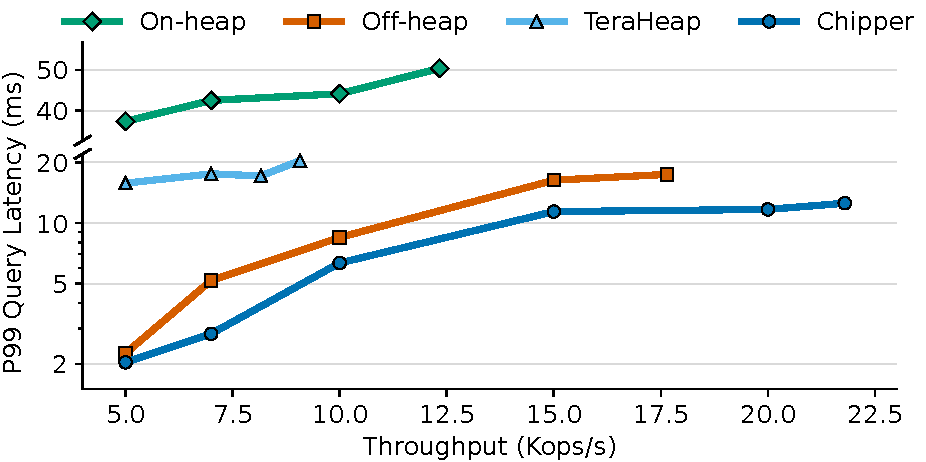
\includegraphics[width=0.5\linewidth]{chipper/figures/motiv/hbase_lat_xput_workloadc.pdf}
	\caption{P99 query latency versus achieved throughput for HBase with YCSB workload~C under the same DRAM budget.}
	\label{chipper:fig:motiv}
\end{figure}

We motivate the need for a storage-backed heap in low-pause garbage collectors using result caches of latency-sensitive applications.
We show that existing approaches either limit cache size or introduce S/D overheads that increase application tail latency.
We use HBase with YCSB~\cite{cooper:ycsb} workload~C, a read-only workload that stresses the block cache of HBase.
We show P99 query latency (Figure~\ref{chipper:fig:motiv}) of \chipperName{} against three baselines under the same DRAM budget: a DRAM-constrained on-heap cache, a storage-backed off-heap cache, and TeraHeap.
We describe the experimental baselines and methodology in \S\ref{chipper:sec:methodology}.

\paragraph{\textbf{On-heap caching is limited by DRAM.}}
The DRAM-constrained on-heap baseline sizes the block cache at 40\% of the heap, the HBase default.
As a result, the cache holds only the data that fits within the DRAM budget, and its hit rate remains at 60\% throughout the run.
Requests that miss in the cache read the corresponding blocks from storage, which dominates tail latency: P99 latency is \SI{37.8}{ms} at \SI{5}{Kops/s} and \SI{43.9}{ms} at \SI{10}{Kops/s}.
The on-heap baseline saturates at \SI{12.3}{Kops/s}, where P99 latency reaches \SI{50.4}{ms}.

\paragraph{\textbf{Off-heap caching incurs S/D cost.}}
The storage-backed off-heap baseline extends the cache beyond DRAM and can accommodate large caches.
Compared with the DRAM-constrained on-heap baseline, it reduces P99 latency by $5.2$--$16.7\times$ across load levels and sustains $1.4\times$ more throughput, reaching \SI{17.6}{Kops/s} instead of \SI{12.3}{Kops/s}.
However, HBase stores cached data blocks in serialized form, requiring deserialization and a copy into the heap on every cache hit.
S/D account for up to 30\% of the request path.
As load increases, the S/D overhead becomes more pronounced: P99 latency rises from \SI{2.3}{ms} at \SI{5}{Kops/s} to \SI{17.4}{ms} at saturation.
Moreover, the off-heap cache requires significant application modifications and extensions; applications without such support cannot extend their caches beyond DRAM without significant development.

\paragraph{\textbf{Existing storage-backed heaps have long GC pauses.}}
TeraHeap extends the managed heap to storage, avoiding both cache misses of on-heap and the S/D cost of off-heap caching.
However, TeraHeap builds on Parallel Scavenge (PS)~\cite{jones:gc_handbook}, a throughput-oriented garbage collector.
Its STW GCs limit application throughput.
The on-heap and off-heap baselines sustain $1.4\times$ and $1.9\times$ more throughput than TeraHeap, respectively.
Compared to the DRAM-constrained on-heap baseline, TeraHeap eliminates cache misses and improves P99 latency by $2.4\times$.
However, compared to the storage-backed off-heap baseline, TeraHeap has $2.4$--$7\times$ higher P99 latency due to its long GC pauses.
TeraHeap has a median GC pause of \SI{824}{ms} and a P99 GC pause of \SI{1.6}{s}, making GC the dominant source of application tail latency.

\paragraph{\textbf{Storage-backed heaps can preserve short GC pauses.}}
Each of the three baselines addresses one part of the problem but introduces another: the on-heap cache is limited by DRAM and incurs cache misses, the off-heap cache incurs S/D cost on every hit, and TeraHeap suffers from long GC pauses.
\chipperName{} is a storage-backed heap managed by a low-pause collector that addresses all three: the cache extends beyond DRAM, cache hits avoid S/D cost, and GC work remains bounded with short GC pauses.
\chipperName{} achieves up to $7\times$ lower tail latency and $1.7\times$ higher throughput than DRAM-constrained on-heap caching, transparently to the application.

\section{\chipperName{} Design}
\label{sec:design}

\chipperName{} provides a storage-backed heap for low-pause collectors that allows large result caches for latency-sensitive applications.
As Figure~\ref{fig:over} shows, \chipperName{} exposes a single managed heap backed by two media: a DRAM heap (DH) and a storage heap (SH) on NVMe SSDs.
DH is the collector's own heap, which is region-based and generational: mutators allocate in the young generation, and the collector promotes objects that survive several young GCs to the old generation.
SH is divided into regions that are mapped in the JVM address space, using memory-mapped I/O (mmio) with the Linux file-backed \texttt{mmap()}.
SH objects retain their managed object layout, so mutators access them directly through ordinary loads and stores, and the OS page cache serves these accesses.
To avoid storage I/O proportional to the size of SH, \chipperName{} fences the collector from following references from DH into SH and scanning the referenced SH objects.
\chipperName{} also maintains SH metadata in DRAM, which tracks where SH holds references into DH and the state of each SH region.

\begin{figure}[t]
	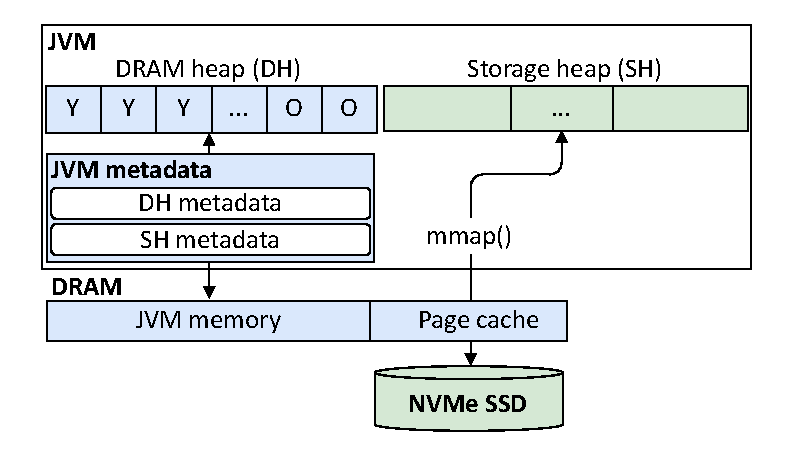
\includegraphics[width=0.6\linewidth]{chipper/figures/design/overview.pdf}
	\caption{\chipperName{} design overview (acronyms: \textbf{Y=}\textbf{Y}oung generation region, \textbf{O=}\textbf{O}ld generation region).}
	\label{fig:over}
\end{figure}

Next, we describe how we design \chipperName{} to work with the three main aspects of low-pause collectors: (1) bounding GC work (\S\ref{sec:distribute}), (2) parallel object evacuation (\S\ref{sec:evacuate}), and (3) separate handling of large objects (\S\ref{sec:nonmovable}).
Finally, we describe how \chipperName{} reclaims space in SH (\S\ref{sec:sh-reclaim}).

\subsection{Bounding GC Work}
\label{sec:distribute}

\chipperName{}'s main function is to migrate objects from DH to SH, allowing the application heap and its result caches to grow beyond the available DRAM.
We refer to objects evacuated during incremental GCs as \emph{regular objects}.
For regular objects, SH migration changes both the amount of DH space reclaimed from a region and the evacuation work required to reclaim that DH space.
Ignoring the additional DH space reclaimed by SH migration can delay migration, while ignoring SH evacuation work can cause the collector to exceed the intended GC work budget.
\chipperName{} therefore extends the collector's region-efficiency model to account for both the DH space reclaimed by SH migration and the corresponding evacuation cost as follows:
%
\begin{equation}
	E(r) = \frac{R_{DH}(r)} {W_{\mathit{evac}}(r)},
\end{equation}
%
where $R_{DH}(r)$ is the DH space reclaimed by evacuating region $r$, and $W_{\mathit{evac}}(r)$ is the corresponding evacuation work.
A higher region efficiency identifies a region that reclaims more DH space for the same evacuation work, or requires less evacuation work to reclaim the same amount of DH space.

\paragraph{\textbf{Estimating reclaimed DH space.}}
Estimating the DH space that a region reclaims requires knowing which of its live objects migrate to SH.
For this object selection, \chipperName{} adopts mechanisms from prior work~\cite{wang:bridgegc,khanh:yak,teraheap,leaksurvivor, kolokasis:teracache,bond:melt,khanh:polar}.
An application labels a cache root object at runtime, and \chipperName{} propagates the label to the objects in its transitive closure during concurrent marking.
We call a labeled object an \emph{SH candidate}.
Live SH candidates contribute to reclaimed DH space even though the SH candidates are not garbage.
After migration to SH, the DH space occupied by an SH candidate becomes available for reuse.
\chipperName{} therefore computes
%
\begin{equation}
	R_{DH}(r) = G(r) + L_{SH}(r),
\end{equation}
%
where, in region $r$, $G(r)$ is the amount of garbage and $L_{SH}(r)$ is the volume of live bytes selected for SH migration.
The remaining live bytes, which are evacuated within DH, are denoted by $L_{DH}(r)$.

Region selection occurs after concurrent marking, so $L_{SH}(r)$ must be available when concurrent marking completes.
\chipperName{} therefore computes $L_{SH}(r)$ during concurrent marking, while the collector scans the object graph to identify live objects.
Similar to prior work~\cite{wu:espresso,teraheap}, \chipperName{} maintains a 64-bit SH-candidate field in each object's header to record whether the object is selected for SH migration.
When concurrent marking identifies a live SH candidate, \chipperName{} adds the object's size to a counter associated with the object's DH region.
At the end of concurrent marking, the counter gives $L_{SH}(r)$, while the remaining live bytes constitute $L_{DH}(r)$.

\chipperName{} does not require all objects in a labeled root's transitive closure to be identified during the same concurrent marking cycle.
An object not identified as an SH candidate during the current concurrent marking cycle remains in DH and may be identified during a later concurrent marking cycle.
Delayed SH-candidate identification affects only SH migration progress; object liveness remains governed by the collector's existing scanning and barrier mechanisms.

\paragraph{\textbf{Estimating evacuation work.}}
Evacuating an object to SH may cost more than evacuating the object within DH because the copy goes through the OS page cache, and the SH evacuation cost depends on whether the target pages are resident.
\chipperName{} therefore computes
%
\begin{equation}
	W_{\mathit{evac}}(r) = C_{DH} \cdot L_{DH}(r) + C_{SH} \cdot L_{SH}(r),
\end{equation}
%
where $C_{DH}$ is the estimated per-byte cost of evacuation within DH, and $C_{SH}$ is the estimated per-byte cost of evacuation from DH to SH.

The per-byte cost of evacuation to SH depends on the state of the OS page cache, so \chipperName{} cannot derive $C_{SH}$ statically.
\chipperName{} therefore estimates $C_{DH}$ and $C_{SH}$ from evacuation measurements.
For each destination, \chipperName{} divides the aggregate evacuation time across GC threads by the total number of bytes evacuated to that destination.
The SH evacuation measurement includes the mmio copy and any synchronous delays incurred through the OS page cache.
For example, accessing a non-resident SH page may trigger a page fault, while OS page-cache pressure may delay a GC thread while the kernel makes page-cache space available.

After each GC that performs SH evacuation, \chipperName{} computes a new per-byte SH evacuation-cost sample and smooths $C_{SH}$ over recent samples to avoid reacting to individual I/O variations.
Before observing the first SH evacuation, \chipperName{} initializes $C_{SH}$ to $C_{DH}$.

\chipperName{} does not prescribe how a collector selects regions for evacuation.
Instead, \chipperName{} provides SH-aware estimates of the DH space reclaimed from each region and the evacuation work required to reclaim that DH space.
A low-pause collector uses the SH-aware estimates to rank regions and to predict the evacuation work of the regions admitted into an incremental GC.

\subsection{Parallel Object Evacuation}
\label{sec:evacuate}

\chipperName{} must preserve evacuation parallelism when migrating objects to SH.
The label of an SH candidate determines the SH region that receives the object, so that \chipperName{} collocates the objects of a cache in SH.
A GC thread may therefore evacuate objects of different labels into different SH regions during one GC, which per-thread allocation state cannot serve: maintaining separate allocation state for every GC thread and for every active SH region would increase DRAM metadata.
\chipperName{} therefore associates an allocation lock with each label-to-region mapping.
GC threads targeting different labels can allocate from different current SH regions in parallel, while GC threads targeting the same label serialize allocation.

\begin{figure}[t]
	\centering
	\subfloat[]{%
		\begin{minipage}[b][5.5cm][c]{0.375\linewidth}
			\centering
			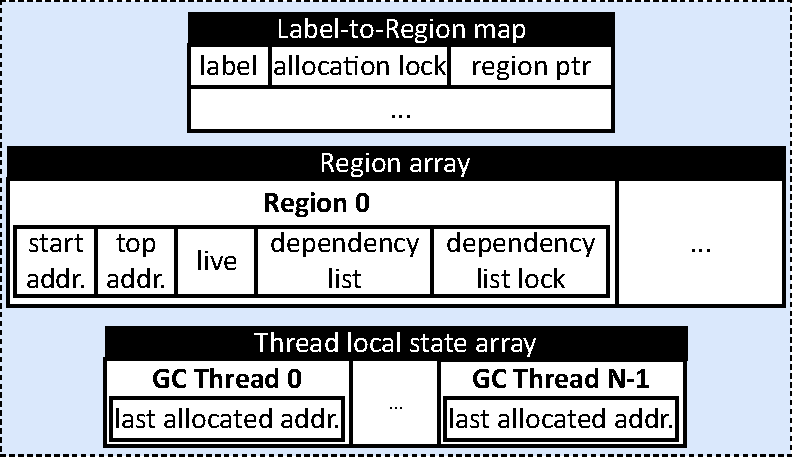
\includegraphics[width=\linewidth]{chipper/figures/design/allocator_meta.pdf}
		\end{minipage}
	}
	\hfill
	\subfloat[]{%
		\begin{minipage}[b][5.5cm][c]{0.6\linewidth}
			\centering
			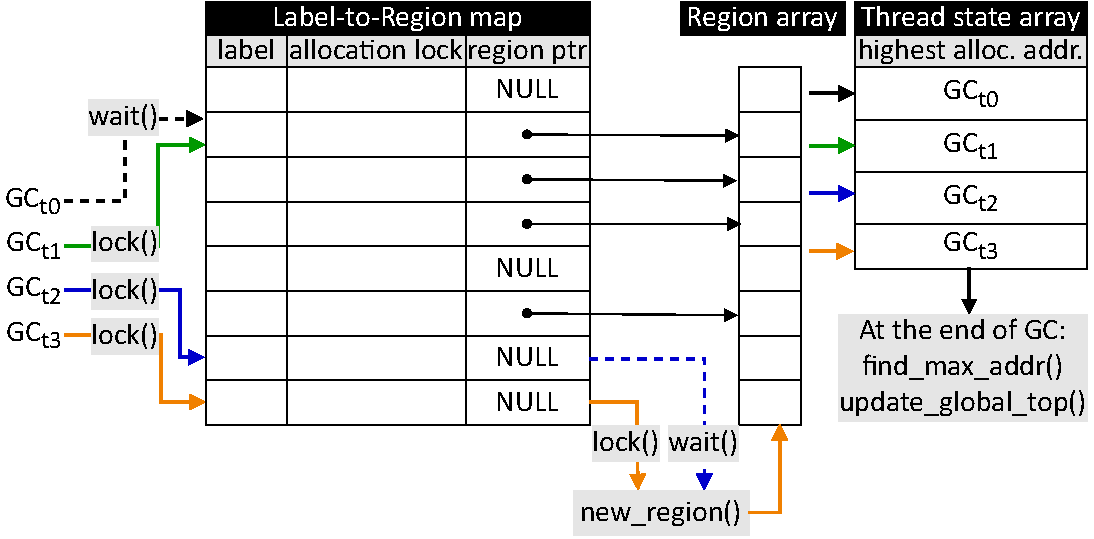
\includegraphics[width=\linewidth]{chipper/figures/design/parallel-allocator.pdf}
		\end{minipage}
	}
	\caption{(a) SH allocator metadata in DRAM and (b) parallel evacuation across multiple SH regions.}
	\label{fig:alloc-meta}
\end{figure}

Figure~\ref{fig:alloc-meta}(a) shows the SH allocator metadata that \chipperName{} maintains in DRAM.
Each entry in the Label-to-Region map contains an allocation lock and a pointer to the current SH region for the corresponding label.
The metadata of each SH region records the allocation position.
Allocating space for an object in SH proceeds in two steps.
First, a GC thread acquires the allocation lock for the label, reserves space in the current SH region, advances the allocation position, and releases the lock.
Second, the GC thread updates its thread-local state to record the highest SH address it has allocated.
At the end of the GC, \chipperName{} determines the highest allocated address across all GC threads and updates the global SH top address if it is lower than this address.
This avoids synchronization on the update of the SH global top address during parallel evacuation.

Figure~\ref{fig:alloc-meta}(b) illustrates how this design enables parallel allocation across multiple SH regions.
GC threads allocating objects with different labels acquire independent allocation locks and can reserve space concurrently.
In contrast, threads allocating objects with the same label must wait for the corresponding allocation lock.
Assigning a new SH region to a label requires global synchronization because the operation modifies the free-region pool shared by all labels.
When a label has no current SH region or the current region lacks sufficient free space, the GC thread acquires the global lock, allocates a new SH region from the free-region pool, and updates the region pointer in the corresponding Label-to-Region map entry.
As illustrated in Figure~\ref{fig:alloc-meta}(b), GC threads $t_2$ and $t_3$ allocate objects with different labels but contend for the \emph{global region allocation lock} because both need to assign a new SH region.
Thus, synchronization is limited to space reservation among threads sharing the same label and global region assignment, allowing allocations to existing regions with different labels to proceed independently.

Evacuation to SH also constrains the collector's forwarding mechanism.
The complete object must be available at the SH destination before the collector publishes that address as the forwarding destination.
Prior storage-backed heaps may stage objects in intermediate DRAM buffers and write the objects asynchronously to storage~\cite{bond:melt,teraheap}.
An intermediate DRAM buffer cannot serve as the final SH destination for collectors that evacuate concurrently with mutators, such as ZGC and Shenandoah, because mutators may access an object immediately after the forwarding destination is published.
\chipperName{} instead uses mmio to copy the object directly to the final SH address through the OS page cache.
After the mmio copy completes, the collector can publish the SH address as the forwarding destination without waiting for dirty pages to be written to the NVMe device; the kernel performs dirty-page write-back later.
For STW collectors, intermediate DRAM buffers are safe while mutators remain stopped, but the GC pause cannot end until all objects are drained from the intermediate buffers and copied to their final SH destinations.

\paragraph{\textbf{Handling concurrent evacuation of the same object.}}
Multiple GC threads may encounter the same SH candidate through different references and attempt to evacuate the object concurrently.
Each GC thread may reserve a different SH destination.
The collector's forwarding mechanism ensures that only one reserved SH destination becomes the object's forwarding destination.
A GC thread whose reserved destination is not selected fills the unused allocation range with a filler object, allowing subsequent SH card scanning to traverse the SH region linearly.
Concurrent evacuation of the same object may therefore consume additional SH space, but avoids additional synchronization on the object-evacuation path.
We quantify this space overhead in \S\ref{chipper:sec:eval}.

\subsection{Handling Large Objects}
\label{sec:nonmovable}

Incremental GCs do not evacuate large objects, so a large SH candidate cannot leave DH through an incremental GC and occupies DRAM while it is live.
Its migration therefore requires a GC that evacuates objects without a GC work budget.
\chipperName{} identifies large SH candidates during concurrent marking, as it does for regular objects, and preserves the SH-candidate state across GCs.
When the collector invokes its mechanism for relieving memory pressure, \chipperName{} migrates the retained large SH candidates.

Migrating a large SH candidate is safe only after the complete object is available at its SH destination and references can resolve to that destination.
\chipperName{} therefore assigns each live large SH candidate an SH destination, integrates the SH destination with the collector's forwarding and reference-update mechanisms, and reclaims the original DH space only after migration completes.
If the collector does not invoke the mechanism for relieving memory pressure, the large SH candidate remains in DH and migration is deferred.

\paragraph{\textbf{Preserving SH-to-DH (backward) references to deferred large objects.}}
Backward references can arise from partial migration of a labeled object graph or from mutator updates.
Regular objects may migrate to SH during incremental GCs while referenced large SH candidates remain in DH awaiting migration.
This partial migration creates backward references from migrated SH objects to large SH candidates that remain in DH.
Mutators may also create new backward references by storing a DH reference into an SH object.
The collector must observe both sources of backward references to preserve the liveness of referenced DH objects and to update the backward references when referenced DH objects move.

Similar to previous work~\cite{teraheap,kolokasis:teraheap_toplas}, \chipperName{} tracks backward references using an SH card table maintained in DRAM, with one byte for each fixed-size segment of SH.
To detect backward references created by mutators, \chipperName{} extends the post-write barrier emitted by the interpreter and the C1 and C2 JIT compilers.
The post-write barrier marks the corresponding SH card \emph{dirty} whenever a mutator updates a reference field in an SH object.
During a GC, GC threads scan dirty SH cards in parallel and process backward references as GC roots.
If a referenced DH object is evacuated, \chipperName{} updates the backward reference to the object's forwarding destination.

Scanning SH cards may access storage-resident objects and incur storage I/O.
To avoid rescanning SH cards whose backward references are irrelevant to a GC, \chipperName{} classifies each scanned SH card according to the referenced DH objects.
For generational collectors, an SH card becomes \emph{clean} if the card contains no backward references, \emph{old} if all backward references point to old generation objects, and \emph{young} if at least one backward reference points to a young generation object.
A young GC can therefore skip clean and old SH cards and scan only SH cards that may contain references relevant to the collection.

Skipping an old SH card is safe only when an incremental GC cannot reclaim an old object referenced by that card.
Large objects require special treatment because a collector may reclaim a dead large object during an incremental GC without evacuating the object.
For example, G1 eagerly reclaims dead large objects during young GCs.
If a backward reference is the only reference keeping a large SH candidate live, skipping the corresponding SH card would hide the backward reference from the collector and could cause premature reclamation.
\chipperName{} therefore classifies an SH card that references a large SH candidate awaiting migration as \emph{young}, regardless of the large object's generation.
The SH card remains \emph{young} until the referenced large SH candidate is migrated to SH or becomes dead.

\subsection{Reclaiming SH Space}
\label{sec:sh-reclaim}

Like prior storage-backed heaps~\cite{leaksurvivor,teraheap}, \chipperName{} reclaims an SH region only when all objects in the region are dead, trading SH capacity for storage I/O.
Reclaiming a partially live SH region would require evacuating the live objects in the region, generating additional storage I/O that can increase application latency.

\paragraph{\textbf{Tracking SH inter-region references.}}
The collector does not scan SH objects during concurrent marking, so SH-region liveness cannot be determined by following references between SH regions directly.
We refer to an SH-to-SH reference whose source and target objects reside in different SH regions as an \emph{inter-region reference}.
Similar to TeraHeap~\cite{teraheap}, \chipperName{} maintains a dependency list for each SH region.
The dependency list records the target SH regions of inter-region references originating from the corresponding source SH region, as shown in Figure~\ref{fig:alloc-meta}(a).
During concurrent marking, \chipperName{} uses these SH-region dependencies to propagate liveness across SH regions without scanning SH objects.

\chipperName{} records SH-region dependencies when inter-region references are created during object evacuation or by mutator updates.
When an object is evacuated to SH, \chipperName{} examines the object's references to SH objects.
For each inter-region reference, \chipperName{} adds the target SH region to the dependency list of the object's destination SH region if the dependency is not already present.
A mutator may subsequently create a new inter-region reference by updating a reference field in an SH object.
When GC threads scan the corresponding dirty SH card, \chipperName{} adds the target SH region to the dependency list of the source SH region if the dependency is not already present.

Multiple GC threads may update dependency lists concurrently.
Each SH region therefore maintains a dependency lock separate from the allocation lock described in \S\ref{sec:evacuate}.
GC threads updating different dependency lists proceed in parallel, while GC threads updating the same dependency list synchronize using the corresponding dependency lock.

\paragraph{\textbf{Reclaiming SH regions.}}
To reclaim SH regions without scanning SH objects, \chipperName{} tracks SH-region liveness using DRAM metadata.
Each SH region maintains a liveness bit in its DRAM metadata, as shown in Figure~\ref{fig:alloc-meta}(a).
At the beginning of concurrent marking, \chipperName{} clears the liveness bit of every allocated SH region.
When concurrent marking encounters a DH-to-SH reference, \chipperName{} sets the liveness bit of the referenced SH region and propagates liveness transitively through the region's dependency list.
Consequently, an SH region becomes live only when the region is reachable from DH, directly or through another live SH region.
Mutually referencing dead SH regions therefore remain dead.

Prior storage-backed heaps determine SH-region liveness while mutators are stopped, whereas \chipperName{} determines SH-region liveness concurrently with mutators.
Concurrent marking must therefore account for the references that mutators overwrite while marking is in progress.
Low pause collectors use snapshot-at-the-beginning (SATB) marking: a barrier records every reference that a mutator overwrites during concurrent marking, and the collector processes the recorded references as part of marking, so that an object reachable when marking began remains live for the marking cycle.
\chipperName{} also processes the DH-to-SH references that the SATB barrier records, so that an SH region reachable when marking began remains live even if a mutator overwrites the last DH reference to it.
% Before finalizing SH-region liveness, \chipperName{} processes SH cards dirtied
% during concurrent marking to account for SH-to-SH references created by mutator
% updates.

At the end of concurrent marking, \chipperName{} examines the liveness bit of every allocated SH region.
An SH region whose liveness bit remains clear contains no live objects, so \chipperName{} resets the region's metadata and makes the entire SH region available for reuse without scanning the region's objects.
SH-region liveness is conservative: a dead SH object remains allocated until every object in the same SH region is dead.
This conservatism affects SH capacity but not correctness.

\section{\chipperName{} Implementation in G1}
\label{chipper:sec:impl}

We implement \chipperName{} in OpenJDK~17 by extending G1, the default garbage collector in OpenJDK.
Four G1 execution paths are relevant to our implementation: young GCs, concurrent marking cycles, mixed GCs, and Full GCs.
Young and mixed GCs evacuate objects during STW pauses.
Young GCs evacuate young regions, while mixed GCs additionally evacuate selected old regions.
A concurrent marking cycle scans objects concurrently with mutators and computes old generation liveness for subsequent mixed GCs.
In G1, young and mixed GCs are the incremental GCs defined in \S\ref{sec:distribute}, humongous objects are the large objects defined in \S\ref{sec:nonmovable}, and Full GC is G1's mechanism for relieving memory pressure.

We next describe how \chipperName{} integrates SH references, SH migration, and SH metadata maintenance in each path.

\paragraph{\textbf{Young GC}}
During a young GC, \chipperName{} must keep SH outside G1's evacuation scan while making backward references visible as roots so that referenced young DH objects remain live.
When object scanning encounters a DH-to-SH reference, \chipperName{} fences the collector from following the reference and scanning the referenced SH object.
GC threads scan \emph{dirty} and \emph{young} SH cards and process backward references through G1's root-evacuation path.
If a referenced DH object is evacuated, G1's existing evacuation path updates the SH reference to the object's forwarding destination.
After scanning an SH card, the GC thread reclassifies the SH card according to the remaining DH targets.

\paragraph{\textbf{Concurrent marking cycle}}
Concurrent marking must expose old generation objects reachable from SH, determine SH-region liveness, and compute the per-region SH-candidate volume required for subsequent Mixed GC region selection.

Old generation objects reachable only from SH would otherwise appear dead to concurrent marking.
\chipperName{} therefore exposes the referenced old generation objects as marking roots before concurrent marking begins.
A concurrent marking cycle starts with a concurrent-start young GC.
During this STW phase, \chipperName{} scans \emph{dirty}, \emph{young}, and \emph{old} SH cards.
For backward references that point to old generation objects, \chipperName{} marks the referenced objects in G1's marking bitmap and pushes the referenced objects onto G1's marking stack.
The referenced old generation objects then participate in subsequent concurrent marking.
Backward references to young objects require no additional marking-root handling because G1 already scans the survivor regions of the concurrent-start young GC as root regions.

The SH-region liveness bits and per-region $L_{SH}(r)$ counters describe a single concurrent marking cycle and must therefore be reset at the beginning of each cycle.
During the concurrent-start pause, before processing roots, \chipperName{} clears the liveness bit of every allocated SH region and resets the per-DH-region $L_{SH}(r)$ counters.
While G1 scans the object graph, \chipperName{} identifies SH candidates and accumulates $L_{SH}(r)$ as described in \S\ref{sec:distribute}.
G1 already maintains the total live bytes of each old region, including SH candidates, so \chipperName{} derives $L_{DH}(r)$ by subtracting $L_{SH}(r)$ from G1's live-byte count.

SH-region liveness must also remain consistent with G1's snapshot-at-the-beginning (SATB) marking semantics.
When concurrent marking encounters a DH-to-SH reference, \chipperName{} marks the referenced SH region live, propagates liveness through the region's dependency list, and fences the collector from following the reference and scanning the referenced SH object.
\chipperName{} also processes DH-to-SH references retained in G1's SATB buffers so that SH regions reachable at the beginning of the concurrent marking cycle remain live.
At remark, \chipperName{} processes SH cards dirtied during concurrent marking, records inter-region dependencies discovered on those cards, and propagates SH-region liveness through the corresponding dependency lists before finalizing SH-region liveness.
SH regions whose liveness bits remain clear can then be reclaimed.
The resulting $L_{SH}(r)$ and $L_{DH}(r)$ values are available for subsequent Mixed GC region selection.

\paragraph{\textbf{Collection-set prediction}}
\chipperName{} must incorporate the SH-aware reclaimed-DH-space and evacuation-work estimates from \S\ref{sec:distribute} into G1's existing old-region selection mechanism without changing the remainder of G1's collection-set policy.

At the end of concurrent marking, when G1 builds the candidate old-region list for subsequent mixed GCs, \chipperName{} computes $E(r)$ for each candidate old region using the $R_{DH}(r)$ and $W_{\mathit{evac}}(r)$ estimates from \S\ref{sec:distribute}.
G1's existing collection-set chooser orders candidate regions using $E(r)$.
When constructing a Mixed GC collection set, G1 predicts the evacuation work of each candidate region as
%
\[
	C_{DH} \cdot L_{DH}(r) +
	C_{SH} \cdot L_{SH}(r)
\]
%
and admits old regions while the predicted pause remains within G1's pause-time target.
The remaining prediction terms and collection-set admission rules remain unchanged.

G1's existing per-byte evacuation-cost estimate provides $C_{DH}$.
\chipperName{} maintains $C_{SH}$ from mixed GCs that perform SH evacuation.
After each such mixed GC, \chipperName{} records the measured per-byte SH evacuation cost and uses the average of the ten most recent samples for subsequent predictions.
Before observing the first SH evacuation, \chipperName{} initializes $C_{SH}$ to $C_{DH}$.

\paragraph{\textbf{Mixed GC}}
During a mixed GC, \chipperName{} exposes backward references as evacuation roots, migrates selected SH candidates, and records the resulting SH reference metadata.

Before evacuation, \chipperName{} scans all non-clean SH cards and processes backward references through G1's root-evacuation path because old SH cards may point to old regions in the collection set.
As G1 evacuates objects from the collection set, \chipperName{} acquires the allocation lock associated with the SH candidate's label-to-region mapping, allocates an SH destination from the current SH region, and copies the SH candidate directly to the reserved SH destination through mmio.

G1 stores an object's forwarding destination in the source object's mark word.
\chipperName{} uses the same mechanism to store the SH address as the forwarding destination.
If multiple GC threads evacuate the same SH candidate, a GC thread whose reserved SH destination is not selected fills the unused allocation range with a filler object.
If SH allocation fails, \chipperName{} evacuates the SH candidate within DH and preserves the object's SH-candidate state for a later GC.

While scanning an object evacuated to SH, \chipperName{} maintains the SH scan boundary and SH reference metadata.
For a DH-to-SH reference, \chipperName{} fences the collector from following the reference and scanning the referenced SH object.
\chipperName{} records inter-region references in the dependency list of the destination SH region while holding the corresponding dependency lock.
Backward references mark the corresponding SH cards.
G1 then continues evacuation through the existing evacuation path.

\paragraph{\textbf{Full GC}}
\chipperName{} uses G1's Full GC to migrate humongous SH candidates whose SH migration has been deferred across incremental GCs, as well as regular SH candidates that mixed GCs have not yet migrated.
Integrating SH migration into Full GC requires \chipperName{} to identify live SH candidates, assign exactly one SH destination to each candidate, redirect references to the assigned SH destinations, and complete the SH copies before reusing the original DH space.

\underline{Identify live candidates and SH regions (marking).}
Full-GC marking must determine both SH-region liveness and which deferred humongous SH candidates remain live.
At the beginning of Full-GC marking, \chipperName{} clears the liveness bit of every allocated SH region.
When marking encounters a DH-to-SH reference, \chipperName{} marks the referenced SH region live and propagates liveness through the region's dependency list.
Full-GC marking also identifies live humongous SH candidates that remain in DH.
Also, \chipperName{} must preserve the object metadata required to migrate live humongous SH candidates later in Full GC.
G1 stores Full-GC forwarding information in the mark word but does not normally move humongous objects, so G1 does not preserve the mark-word state of humongous objects for movement.
For each live humongous SH candidate, \chipperName{} therefore preserves the mark-word state that must survive SH migration before G1 reuses the mark word for forwarding information.
\chipperName{} also ensures that the first DH region occupied by the humongous SH candidate, which contains the object header, participates in subsequent Full-GC processing.
After Full-GC marking, any allocated SH region whose liveness bit remains clear can be reclaimed.

\underline{Prepare for compaction.}
Each live SH candidate requires exactly one SH destination before G1 adjusts object references.
G1's preparation-for-compaction phase normally assigns new DH destinations to objects that will move.
For an SH candidate, \chipperName{} instead allocates an SH destination and records the SH address as the forwarding destination.
\chipperName{} also ensures that a DH region containing an SH candidate participates in compaction even when G1 would otherwise exclude the region based on live-data occupancy.
However, humongous SH candidates require an additional handling phase because a single humongous object may span DH regions processed by different GC threads.
To assign exactly one SH destination, only the GC thread processing the first DH region of the humongous SH candidate performs the allocation.
GC threads processing continuation regions skip the humongous SH candidate.
The GC thread processing the first DH region records the humongous SH candidate on a local stack for later copying.

\underline{Adjust object references.}
After assigning SH destinations, G1's reference-adjustment phase redirects references to the recorded forwarding destinations.
References to SH candidates therefore resolve to the assigned SH destinations.
Mutators remain stopped during Full GC, and no GC thread reads object contents from an SH destination during reference adjustment.
The complete SH copy therefore does not need to be available while G1 updates references.
\chipperName{} also maintains SH reference metadata created by the new object locations.
\chipperName{} records dependencies for newly created inter-region references and marks SH cards for newly created backward references.
\chipperName{} also scans existing non-clean SH cards and updates backward references whose DH targets receive new forwarding destinations.

\underline{Heap compaction.}
After reference adjustment, \chipperName{} must materialize the complete objects at the assigned SH destinations before reclaiming the original DH space and resuming mutators.
References have already been adjusted and mutators remain stopped, so \chipperName{} can stage SH copies in intermediate DRAM buffers and write the buffered objects to SH asynchronously, unlike incremental evacuation (\S\ref{sec:evacuate}).
Regular SH candidates are copied as part of G1's regular compaction traversal.
G1 compacts each region toward lower addresses in address order, so no object overwrites a regular SH candidate before \chipperName{} copies the SH candidate to the assigned SH destination.
However, humongous SH candidates follow a different copying path because G1's regular compaction traversal does not visit humongous objects.
Each GC thread therefore drains the local stack populated during preparation for compaction and copies the recorded humongous SH candidates to the assigned SH destinations.
\chipperName{} restores the preserved object metadata in the SH copies and waits for all outstanding SH writes to complete before reclaiming the corresponding DH space and resuming mutators.

\section{Experimental Methodology}
\label{chipper:sec:methodology}

Our evaluation answers four questions:

\begin{enumerate}
	\item How does \chipperName{} improve application tail latency compared with a DRAM-limited on-heap cache, a storage-backed off-heap cache, and TeraHeap under the same DRAM budget (\S\ref{sec:eval-latency})?

	\item How does \chipperName{}'s SH-aware region-efficiency model affect application tail latency (\S\ref{sec:eval-selection})?

	\item How does SH allocation-lock granularity affect \chipperName{}'s Mixed GC performance and application tail latency (\S\ref{sec:eval-scalability})?

	\item What is the performance cost of migrating large objects during Mixed GCs compared with deferring their migration to Full GC (\S\ref{sec:eval-large})?

\end{enumerate}

\paragraph{\textbf{Experimental platform}}
We use a dual-socket server with two Intel Xeon E5-2630~v3 CPUs at \SI{2.4}{GHz}, with 16 physical cores in total and hyper-threading enabled, and \SI{256}{GB} of DDR4 DRAM.
The server runs Ubuntu 24.04 with Linux kernel 6.8.
It has three PCIe NVMe SSDs: one \SI{4}{TB} Lexar NM790 and two \SI{2}{TB} Samsung PM983 devices configured as RAID~0.
To reduce variability, we disable swap, set the CPU frequency governor to \emph{performance}, and use the default kernel settings for page-cache write-back.

\begin{table*}[t]
	\small
	\caption{Baselines compared with \chipperName{} and the applications used to evaluate each baseline.
		\textbf{N/A} indicates that an application does not provide a storage-backed off-heap cache.}
	\label{tab:configs}
	\begin{tabular}{@{}lccc cccc@{}}
		\toprule
		                   &               &                   &                            & \multicolumn{4}{c}{\textbf{Application}}                                                     \\
		\cmidrule(l){5-8}
		\textbf{Baselines} & \textbf{DRAM} & \textbf{NVMe SSD} & \textbf{Garbage collector} & \textbf{OpenSearch}                      & \textbf{Lucene} & \textbf{Spark} & \textbf{HBase} \\
		\midrule
		On-heap            & Heap          & --                & G1                         & \checkmark                               & \checkmark      & \checkmark     & \checkmark     \\
		Off-heap           & Heap          & Off-heap          & G1                         & \checkmark                               & N/A             & \checkmark     & \checkmark     \\
		TeraHeap           & DH            & SH                & Parallel Scavenge          & \checkmark                               & \checkmark      & \checkmark     & \checkmark     \\
		\bottomrule
	\end{tabular}
\end{table*}

\paragraph{\textbf{Baselines}}
We compare \chipperName{} against three baselines that differ in where cached data resides and how the cache is managed: on-heap, off-heap, and TeraHeap~\cite{teraheap}.
The on-heap baseline stores cached data in the managed heap and is therefore limited by the available DRAM.
The off-heap baseline extends cache capacity to storage, but accesses to the storage-backed portion of the cache incur S/D costs.
The storage-backed portion of the off-heap cache and the SH of both TeraHeap and \chipperName{} reside on the RAID~0 device.
TeraHeap and \chipperName{} label the root object of the same cache entry in each application, keeping the set of storage-backed objects consistent across the two systems.
\chipperName{} and all baselines run on OpenJDK~17.
\chipperName{} and the baselines that use G1 use G1's default settings, including a pause-time target of \SI{200}{ms} and thirteen GC threads, as determined by the number of CPU cores available to the application.
TeraHeap uses Parallel Scavenge with the same thirteen GC threads.
Table~\ref{tab:configs} summarizes the baselines.

\begin{table}[t]
	\small
	\setlength{\tabcolsep}{5pt}
	\caption{Workloads, datasets, and memory configuration.
		Heap is the managed heap of the on-heap and off-heap baselines, and DH is the DRAM heap of TeraHeap and \chipperName{}.}
	\label{tab:workloads}
	\begin{tabular}{@{}llccc@{}}
		\toprule
		\textbf{Application}   & \textbf{Workload} & \textbf{Dataset}    & \textbf{Heap / DH} & \textbf{DRAM}       \\
		                       &                   & \textbf{(GB)}       & \textbf{(GB)}      & \textbf{(GB)}       \\
		\midrule
		OpenSearch             & NYC Taxi          & 27                  & 2                  & 4                   \\
		Lucene                 & NYC Taxi          & 27                  & 8                  & 16                  \\
		Spark                  & Yahoo Streaming   & --                  & 1                  & 4                   \\
		\multirow{2}{*}{HBase} & YCSB (Workload A) & \multirow{2}{*}{60} & \multirow{2}{*}{8} & \multirow{2}{*}{16} \\
		                       & YCSB (Workload F) &                     &                    &                     \\
		\bottomrule
	\end{tabular}
\end{table}

\paragraph{\textbf{Applications and workloads.}}
We evaluate \chipperName{} with four applications that use result caches.
Table~\ref{tab:configs} shows which baselines we compare against for each application and Table~\ref{tab:workloads} summarizes the workloads and datasets.

(1)~OpenSearch~2.19~\cite{opensearch} is a search engine that caches search-request results for each shard in a request cache.
We use the NYC Taxi workload from the OpenSearch Benchmark~\cite{opensearch-benchmark}, whose index contains 165{,}346{,}692 documents and occupies \SI{27}{GB}.
We use the query mix from~\cite{opensearch:tiered-cache}, designed to exercise the request cache, and issue queries with 13 clients.
For the off-heap baseline, we use the tiered request cache with its storage tier on the NVMe SSD.

(2)~Lucene~9.12~\cite{mccandless:lucene} is a search library that caches the results of frequently executed query filters in a query cache.
We exercise the query cache through the OpenSearch server using a separate set of queries from the workload repository~\cite{opensearch:query_cache_benchmarks} that stress the query cache, issued by 8 clients.
Lucene does not provide a storage-backed tier for its query cache, so we compare \chipperName{} only against the on-heap baseline and TeraHeap.

(3)~Spark~3.3~\cite{zaharia:spark} is a data-processing framework that caches intermediate datasets (RDDs) for reuse across computations.
We use the Yahoo Streaming Benchmark~\cite{chintapalli:yahoo} on Spark DStreams, which models an online advertising analytics workload.
Events are generated at a controlled rate and ingested through Kafka, and each event contains an advertisement identifier and an event type.
The application filters view events and performs a lookup in Redis to map each advertisement to its campaign.
It then applies a sliding window over the records produced by the Redis join and persists these records in Spark's cache.
We use a \SI{4}{s} batch interval, a \SI{300}{s} window, and a \SI{4}{s} slide, so each full window contains 75 batch RDDs.
Consecutive windows reuse 74 of the 75 cached batch RDDs, or 98.7\% of the cached data, creating substantial reuse of long-lived objects in the Spark heap.
For each window, the application aggregates the number of views per campaign and writes the resulting counts and completion timestamps to Redis.
The on-heap baseline, TeraHeap, and \chipperName{} cache RDDs using \texttt{MEMORY\_ONLY}, while the off-heap baseline uses \texttt{MEMORY\_AND\_DISK}, which spills serialized RDD partitions to the NVMe SSD.

(4)~HBase~2.6~\cite{vohra:hbase} is a key-value store that caches data blocks read from store files in a block cache.
We evaluate HBase with two mixed workloads from YCSB~\cite{cooper:ycsb}: Workload~A, with 50\% reads and 50\% updates, and Workload~F, with 50\% reads and 50\% read-modify-writes (RMW).
We load 60 million records (\SI{60}{GB}) and run each workload with 128 client threads.
For the off-heap baseline, we use BucketCache with the mmap file I/O engine on the NVMe SSD, which, like \chipperName{}, accesses storage through the OS page cache.

\paragraph{\textbf{Memory configuration}}
We derive the memory configuration of each application from the size of its cached data, so that every configuration operates under the same DRAM budget and the same cache capacity in DRAM.
We first size the on-heap cache to hold 5\% of the cached data, which models deployments in which the working set grows faster than the DRAM a server provides.
We then derive the heap from the on-heap cache size, because each application sizes its cache as a fraction of the heap: the block cache in HBase uses 40\% of the heap and the request cache in OpenSearch uses 1\%, both default values, while we configure Lucene's query cache to 10\% of the heap, its default, and Spark's storage fraction to 50\%.
Finally, we set the DRAM budget to twice the heap for HBase, OpenSearch, and Lucene, as their documentation recommends, which leaves the remaining DRAM for the OS page cache.
For Spark we add \SI{3}{GB} to the heap for the driver and the page cache.
Table~\ref{tab:workloads} reports the resulting sizes.
We enforce the budget with a \emph{cgroup} memory limit that accounts for the managed heap, native memory, and the OS page cache, so configurations that place data on storage cannot use additional DRAM through the page cache.

\paragraph{\textbf{Metrics}}
We report the P99 latency and the throughput that each workload generator measures: YCSB for HBase, the OpenSearch Benchmark for OpenSearch and Lucene, and the Yahoo Streaming Benchmark for Spark.
For GC metrics, we enable unified JVM logging (\texttt{-Xlog:gc*}) and extract the number of GCs, their type, their pause times.
\chipperName{} also reports the volume of data it migrates to SH in each GC.

\section{Evaluation}
\label{chipper:sec:eval}

\subsection{Application Tail Latency Vs Throughput}
\label{sec:eval-latency}

\begin{figure*}[t]
	\centering

	% Legend
	
\includegraphics[width=.4\linewidth]
	{chipper/figures/overall/overall-chipper-legend.pdf}

	\vspace{-0.5em}

	% =========================================================
	% First row: 5 plots
	% =========================================================
	\subfloat[OpenSearch]{
		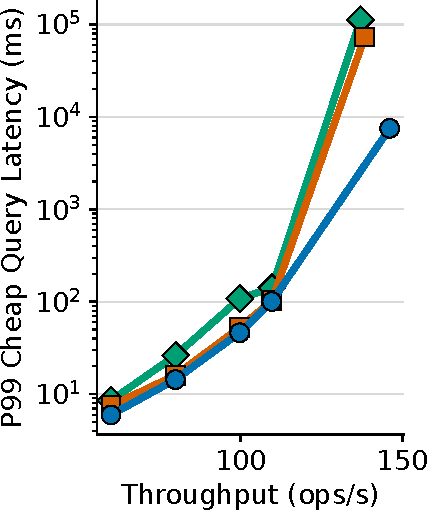
\includegraphics[width=.19\linewidth]
		{chipper/figures/overall/opensearch-chipper-tip-amount.pdf}
		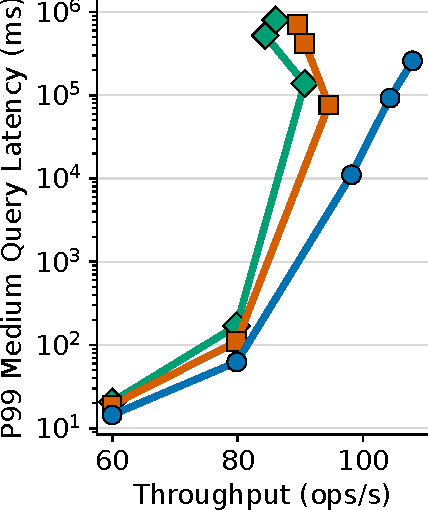
\includegraphics[width=.19\linewidth]
		{chipper/figures/overall/opensearch-chipper-date-histogram-agg.pdf}
		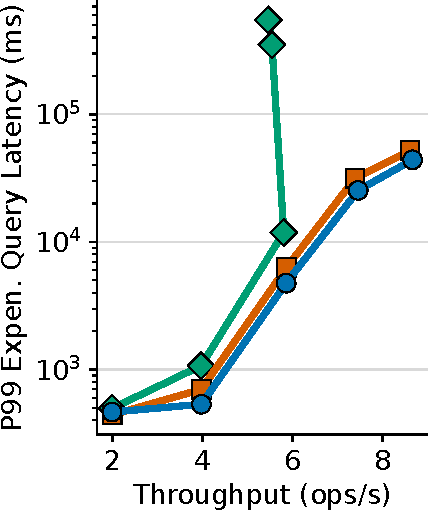
\includegraphics[width=.19\linewidth]
		{chipper/figures/overall/opensearch-chipper-date-histogram-tz.pdf}
	}
	\hspace{-0.8em}
	\subfloat[Lucene]{
		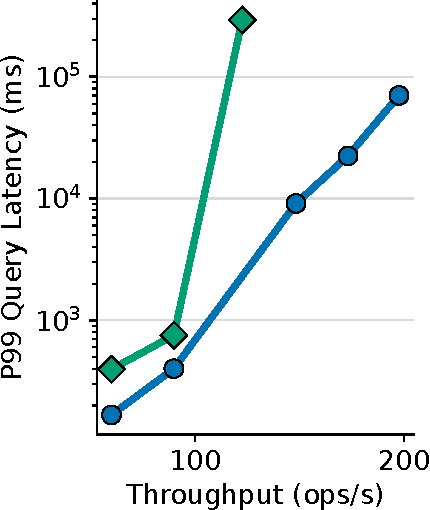
\includegraphics[width=.19\linewidth]
		{chipper/figures/overall/lucene-chipper.pdf}
	}
	\hspace{-0.8em}
	\subfloat[Spark]{
		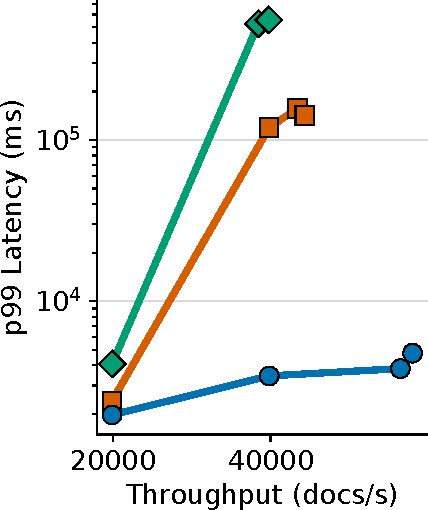
\includegraphics[width=.20\linewidth]
		{chipper/figures/overall/spark-streaming-chipper.pdf}
	}

	\vspace{0.4em}

	% =========================================================
	% Second row: 4 plots
	% =========================================================
	\subfloat[HBase-Workload A]{
		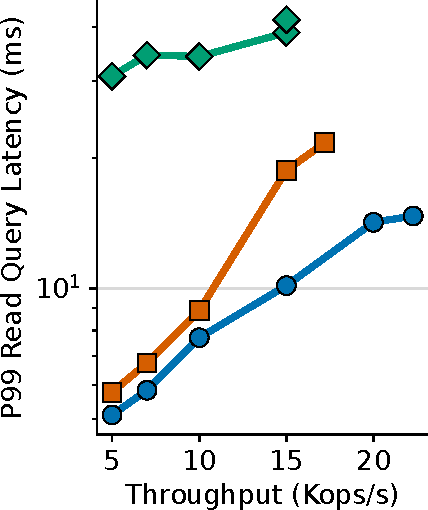
\includegraphics[width=.195\linewidth]
		{chipper/figures/overall/hbase-workloada-chipper-read.pdf}
		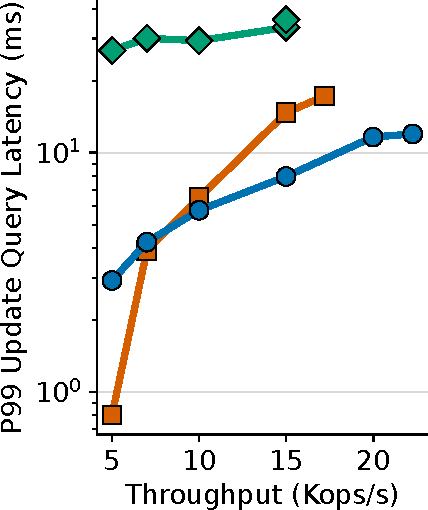
\includegraphics[width=.195\linewidth]
		{chipper/figures/overall/hbase-workloada-chipper-update.pdf}
	}
	\hspace{-0.8em}
	\subfloat[HBase-Workload F]{
		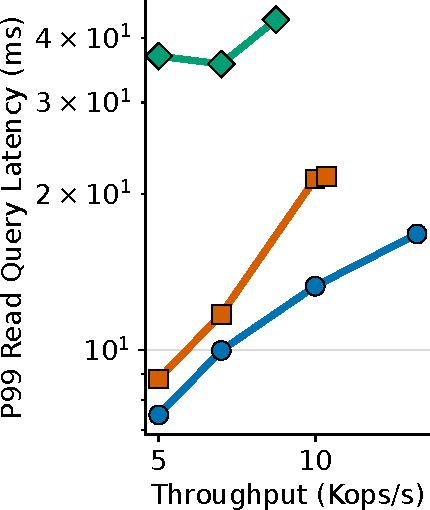
\includegraphics[width=.19\linewidth]
		{chipper/figures/overall/hbase-workloadf-chipper-read.pdf}
		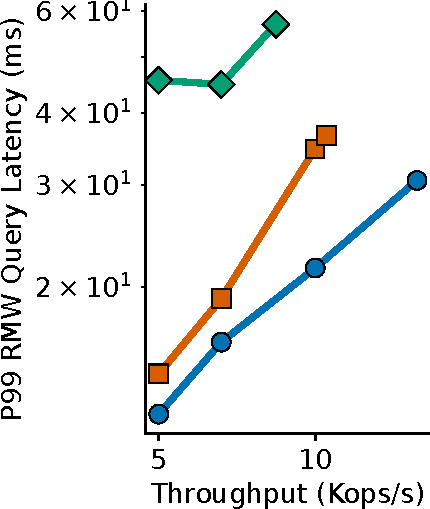
\includegraphics[width=.19\linewidth]
		{chipper/figures/overall/hbase-workloadf-chipper-rmw.pdf}
		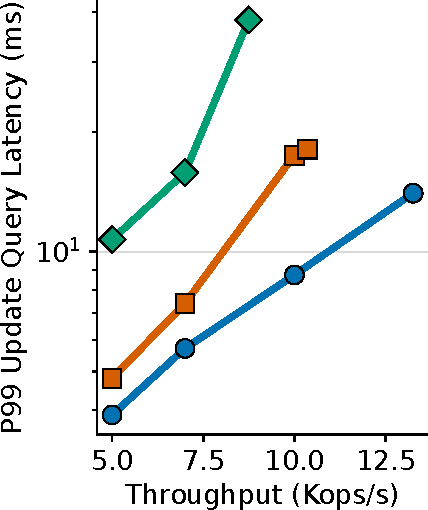
\includegraphics[width=.19\linewidth]
		{chipper/figures/overall/hbase-workloadf-chipper-update.pdf}
	}

	\caption{P99 application latency versus achieved throughput for OpenSearch, Lucene, Spark Streaming, and HBase using on-heap caches, off-heap caches, and \chipperName{}.}
	\label{fig:overall-onheap-offheap-chipper}
\end{figure*}

\paragraph{\textbf{Comparison with on-heap and off-heap caches}}
In this section we evaluate \chipperName{} compared to on-heap and off-heap caching approaches.

Figure~\ref{fig:overall-onheap-offheap-chipper}(a) shows the OpenSearch results, where cheap, medium, and expensive queries run together.
For cheap queries at 110~ops/s, \chipperName{} reduces P99 latency by 29\% over on-heap caching and by 2\% over off-heap caching.
For medium queries at 80~ops/s, \chipperName{} reduces P99 latency by 63\% compared with on-heap caching and by 43\% compared with off-heap caching.
For expensive queries at 6~ops/s, the corresponding reductions are 60\% and 25\%.
The larger gains over on-heap caching come from fewer cache misses: \chipperName{} achieves a 70\% hit rate versus 6\% on-heap, reducing query recomputation.
This matters more as query cost increases.
Compared with off-heap caching, \chipperName{} avoids the S/D cost of accessing cached results while still providing large cache capacity.

Figure~\ref{fig:overall-onheap-offheap-chipper}(b) shows the results for Lucene.
At 90~ops/s, \chipperName{} reduces P99 query latency from 754~ms to 401~ms, a 47\% reduction compared with the on-heap configuration.
As load increases, the on-heap configuration reaches only 123~ops/s before P99 latency increases to 293~s, whereas \chipperName{} continues scaling to 198~ops/s.
At these respective highest measured throughputs, \chipperName{} achieves $1.61\times$ higher throughput while maintaining $4.17\times$ lower P99 latency.
This improvement follows from the larger effective query-cache capacity provided by SH.
\chipperName{} achieves an 88\% cache hit rate, compared with 37\% for the on-heap configuration, reducing query recomputation.

The difference is particularly large for Spark Streaming in Figure~\ref{fig:overall-onheap-offheap-chipper}(c).
At approximately 40K~docs/s, \chipperName{} achieves a P99 latency of 3.4~s, compared with 119.1~s for off-heap caching and 556.0~s for on-heap caching.
Thus, \chipperName{} reduces P99 latency by $34.7\times$ relative to off-heap caching and by $161.8\times$ relative to on-heap caching.
The on-heap configuration suffers from both limited cache capacity and high GC pressure, while the off-heap configuration avoids much of the GC overhead but incurs about 50\% S/D overhead.
By keeping cached RDDs as managed objects in SH, \chipperName{} avoids this S/D overhead while also reducing GC pressure in DH.
\chipperName{} also sustains approximately 58K~docs/s, compared with 44K~docs/s for off-heap caching and 40K~docs/s for on-heap caching, corresponding to approximately $1.31\times$ and $1.46\times$ higher throughput, respectively.

Figures~\ref{fig:overall-onheap-offheap-chipper}(d) and \ref{fig:overall-onheap-offheap-chipper}(e) show the HBase results.
For Workload A at 15K~ops/s, \chipperName{} reduces P99 read latency to 10.2~ms, 46\% lower than off-heap caching and 74--76\% lower than on-heap caching.
For updates, \chipperName{} achieves 8.0~ms P99 latency, reducing latency by 46\% over off-heap caching and 76--78\% over on-heap caching.
\chipperName{} also reaches 22.3K~ops/s, compared with 17.2K~ops/s for off-heap and 15.0K~ops/s for on-heap caching, providing $1.29\times$ and $1.48\times$ higher throughput, respectively.
For Workload F at 10K~ops/s, \chipperName{} reduces P99 latency relative to off-heap caching by 38\% for reads, 38\% for read-modify-write operations, and 50\% for updates.
At 7K~ops/s, where all configurations are directly comparable, \chipperName{} reduces P99 latency relative to on-heap caching by 72\%, 64\%, and 64\% for the same operations.
\chipperName{} reaches 13.3K~ops/s, compared with 10.4K~ops/s for off-heap and 8.7K~ops/s for on-heap caching.
The higher cache hit rate of \chipperName{}, 90\% compared with 60\% on-heap, reduces block-cache misses and the resulting storage accesses.

\begin{figure*}[t]
	\centering

	% Legend
	
\includegraphics[width=.25\linewidth]
	{chipper/figures/overall/overall-tera-vs-chipper-legend.pdf}

	\vspace{-0.5em}

	% =========================================================
	% First row: 5 plots
	% =========================================================
	\subfloat[OpenSearch]{
		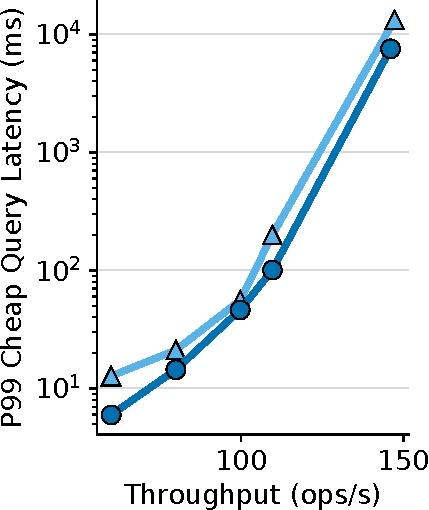
\includegraphics[width=.19\linewidth]
		{chipper/figures/overall/opensearch-tera-vs-chipper-tip-amount.pdf}
		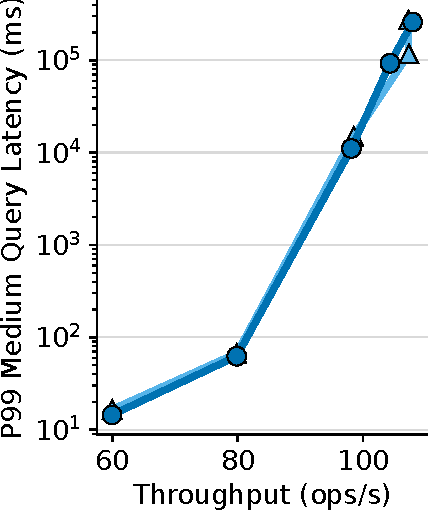
\includegraphics[width=.19\linewidth]
		{chipper/figures/overall/opensearch-tera-vs-chipper-date-histogram-agg.pdf}
		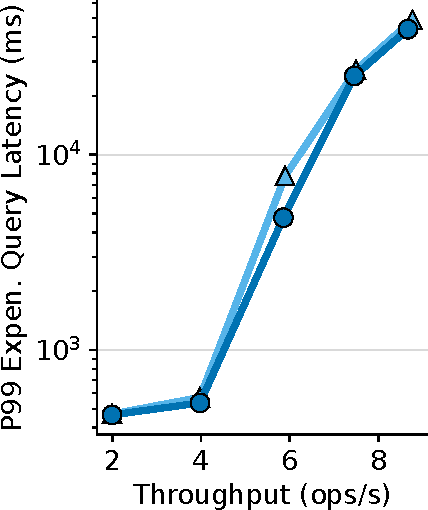
\includegraphics[width=.19\linewidth]
		{chipper/figures/overall/opensearch-tera-vs-chipper-date-histogram-tz.pdf}
	}
	\hspace{-0.8em}
	\subfloat[Lucene]{
		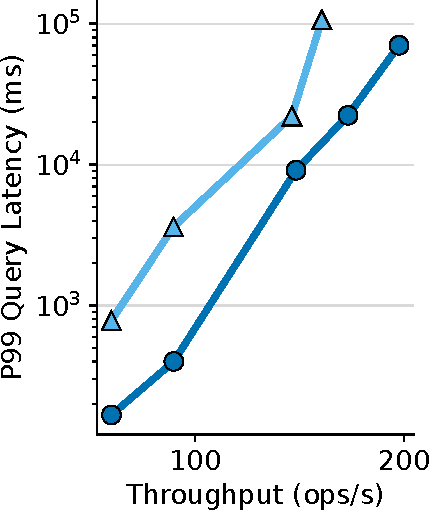
\includegraphics[width=.19\linewidth]
		{chipper/figures/overall/lucene-tera-vs-chipper.pdf}
	}
	\hspace{-0.8em}
	\subfloat[Spark]{
		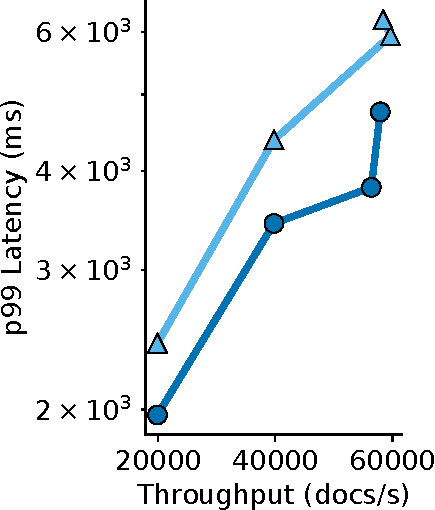
\includegraphics[width=.20\linewidth]
		{chipper/figures/overall/spark-streaming-tera-vs-chipper.pdf}
	}

	\vspace{0.4em}

	% =========================================================
	% Second row: 4 plots
	% =========================================================
	\subfloat[HBase-Workload A]{
		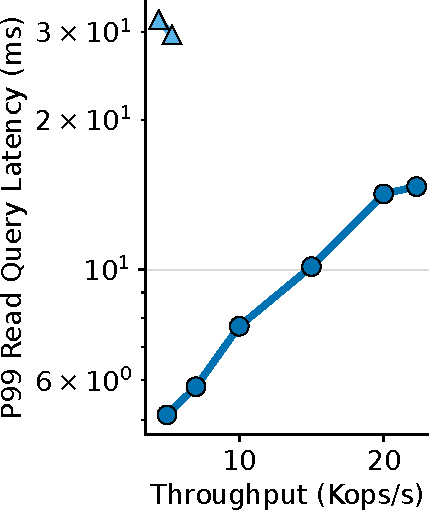
\includegraphics[width=.19\linewidth]
		{chipper/figures/overall/hbase-workloada-tera-vs-chipper-read.pdf}
		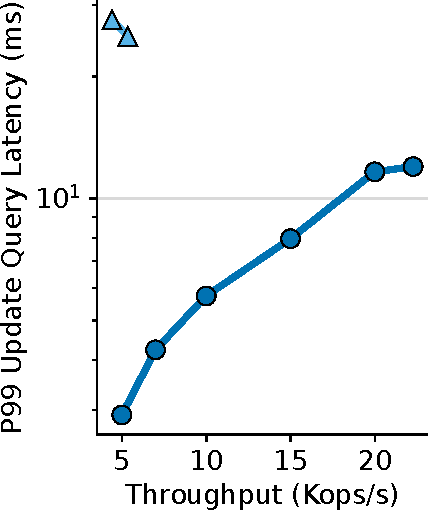
\includegraphics[width=.19\linewidth]
		{chipper/figures/overall/hbase-workloada-tera-vs-chipper-update.pdf}
	}
	\hspace{-0.8em}
	\subfloat[HBase-Workload F]{
		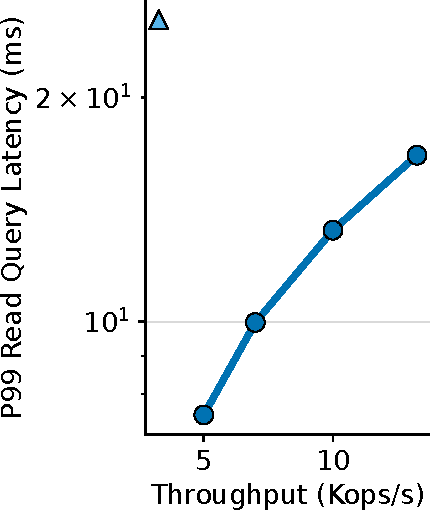
\includegraphics[width=.19\linewidth]
		{chipper/figures/overall/hbase-workloadf-tera-vs-chipper-read.pdf}
		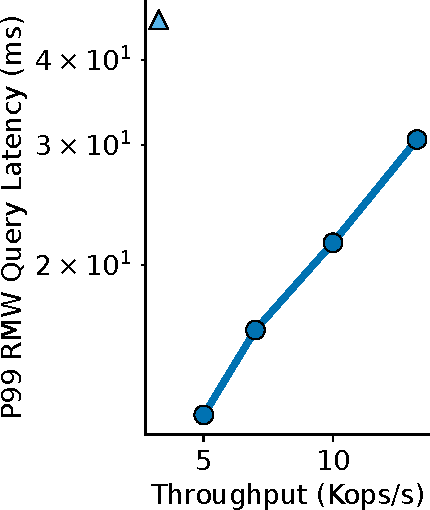
\includegraphics[width=.19\linewidth]
		{chipper/figures/overall/hbase-workloadf-tera-vs-chipper-rmw.pdf}
		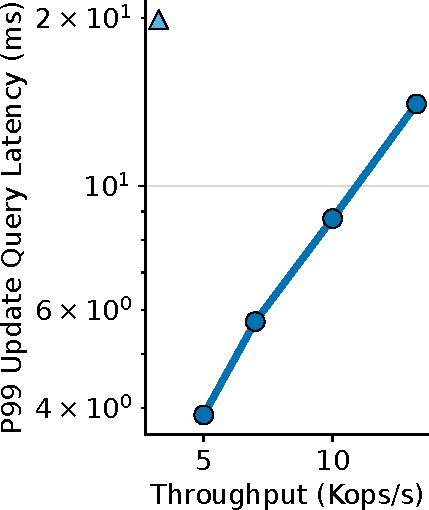
\includegraphics[width=.19\linewidth]
		{chipper/figures/overall/hbase-workloadf-tera-vs-chipper-update.pdf}
	}

	\caption{P99 application latency versus achieved throughput for OpenSearch, Lucene, Spark Streaming, and HBase using TeraHeap and \chipperName{}.}
	\label{fig:overall-tera-vs-chipper}
\end{figure*}

\begin{figure*}[t]
	\centering

	% Legend
	
\includegraphics[width=.25\linewidth]
	{chipper/figures/overall/gc_pauses_legend.pdf}

	\vspace{-0.5em}

	\subfloat[OpenSearch]{
		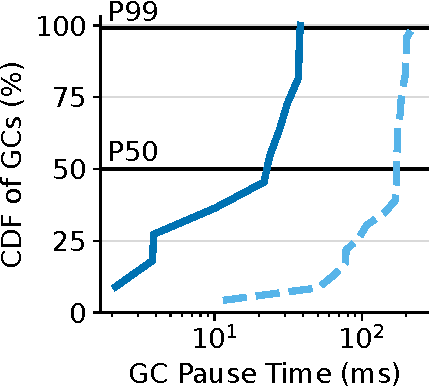
\includegraphics[width=.20\linewidth]
		{chipper/figures/overall/opensearch_gc_pauses_chipper_th_cdf.pdf}
	}
	\subfloat[Spark]{
		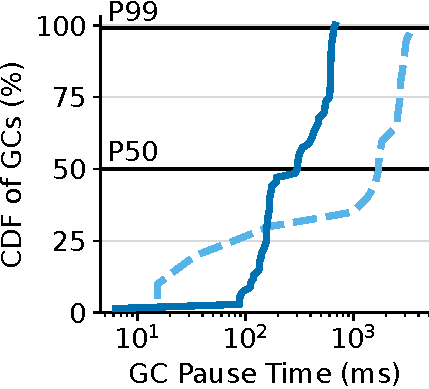
\includegraphics[width=.20\linewidth]
		{chipper/figures/overall/spark_gc_pauses_chipper_th_cdf.pdf}
	}
	\subfloat[HBase-Workload A]{
		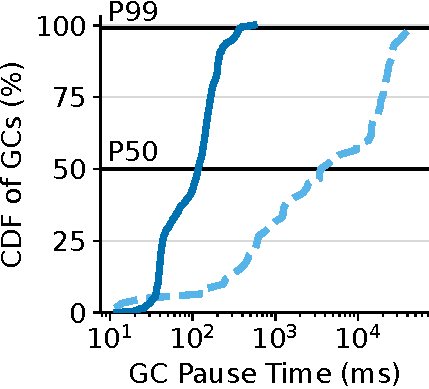
\includegraphics[width=.20\linewidth]
		{chipper/figures/overall/hbase-workloada_gc_pauses_chipper_th_cdf.pdf}
	}
	\subfloat[HBase-Workload F]{
		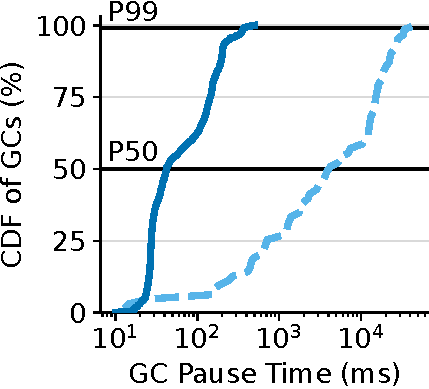
\includegraphics[width=.20\linewidth]
		{chipper/figures/overall/hbase-workloadf_gc_pauses_chipper_th_cdf.pdf}
	}

	\caption{GC pause-time distributions for TeraHeap Full GCs and \chipperName{} Mixed GCs in OpenSearch, Spark Streaming, and HBase Workloads A and F.}
	\label{fig:gc_pauses_chipper_vs_teraheap}
\end{figure*}

\paragraph{\textbf{Comparison with state-of-the-art storage-backed heaps}}
We next compare \chipperName{} with TeraHeap to isolate the benefit of integrating a storage-backed heap with a low-pause collector.
Figure~\ref{fig:overall-tera-vs-chipper} shows the resulting application-level differences.
For OpenSearch, the two systems achieve similar performance because GC activity is low.
For Lucene at 90~ops/s, \chipperName{} achieves $9\times$ lower P99 query latency, reducing it from 3.6~s to 0.4~s, and reaches 198~ops/s compared with 161~ops/s for TeraHeap.
For Spark at 40K~docs/s, \chipperName{} achieves $1.28\times$ lower P99 latency, reducing it from 4.38~s to 3.44~s.
The largest throughput differences occur for HBase, where \chipperName{} reaches 22.3~Kops/s versus 5.4~Kops/s for Workload A and 13.3~Kops/s versus 3.3~Kops/s for Workload F, providing $4.2\times$ and $4.1\times$ higher throughput, respectively.

Figure~\ref{fig:gc_pauses_chipper_vs_teraheap} explains these application-level differences through the corresponding GC pause distributions.
For OpenSearch, \chipperName{} reduces the P99 GC pause from 221~ms to 38~ms, but the small number of collections limits their impact on application latency.
For Spark, \chipperName{} reduces the median GC pause from 1.72~s to 303~ms and the P99 from 3.54~s to 659~ms, both by more than $5\times$.
The difference is larger for HBase.
For Workload A, \chipperName{} reduces the median GC pause from 3.90~s to 117~ms and the P99 from 43.8~s to 374~ms, corresponding to $33\times$ and $117\times$ reductions.
For Workload F, the corresponding reductions are from 4.23~s to 42~ms at the median and from 37.7~s to 370~ms at P99, over $100\times$ in both cases.

\subsection{Effectiveness of SH-Aware Region Ranking}
\label{sec:eval-selection}

\begin{figure}[h]
	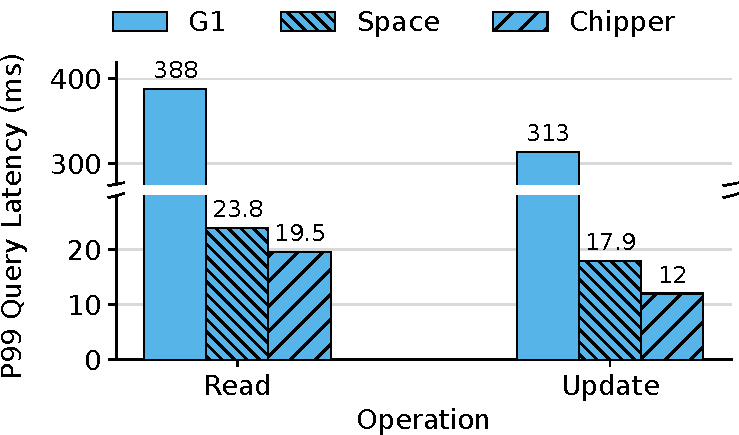
\includegraphics[width=.4\linewidth]{chipper/figures/eval/model/p99_query.pdf}
	\caption{P99 query latency for read and update operations in HBase Workload A under the three region-efficiency models used to rank candidate regions for collection.}
	\label{fig:model-p99}
\end{figure}

We evaluate how effectively \chipperName{}'s SH-aware region-efficiency model ranks candidate regions for collection and how this choice affects application tail latency.
We compare three region-efficiency models while keeping the rest of the system unchanged.
The G1 model uses G1's original region efficiency, which considers garbage reclaimed from a region and the predicted cost of evacuating its live objects within DH.
The Space model additionally accounts for the DH space reclaimed when live SH-candidate objects are evacuated to SH, without considering their evacuation overhead.
The \chipperName{} model accounts for both the additional DH space reclaimed through evacuation to SH and the higher evacuation cost of SH-bound objects.

Figure~\ref{fig:model-p99} shows the resulting P99 query latency for HBase Workload A.
For read operations, \chipperName{} achieves $19.9\times$ lower P99 latency than the G1 model and $1.22\times$ lower P99 latency than the Space model, while for update operations the corresponding improvements are $26.1\times$ and $1.49\times$.
Table~\ref{tab:model-gc} shows that these application-level differences follow from substantially different GC behavior.
The G1 model triggers 89 Full GCs, whereas neither the Space model nor the \chipperName{} model triggers a Full GC.
Compared with the G1 model, Table~\ref{tab:model-gc} shows that \chipperName{} reduces total Mixed GC time by $14.1\times$, the median Mixed GC pause by $3.7\times$, the P90 by $7.3\times$, the P99 by $5.6\times$, and the maximum pause by $5.9\times$.
Compared with the Space model, Table~\ref{tab:model-gc} shows that \chipperName{} performs 34 more Mixed GCs but still reduces total Mixed GC time by $1.09\times$, the median pause by $1.50\times$, the P90 by $1.16\times$, and the maximum pause by $1.93\times$.
The P99 Mixed GC pause is similar for the Space and \chipperName{} models, differing by only $1.02\times$.

\begin{table*}[h]
	\setlength{\aboverulesep}{0pt}
	\setlength{\belowrulesep}{0pt}
	\centering
	\small
	\setlength{\tabcolsep}{4pt}
	\renewcommand{\arraystretch}{1.05}
	\caption{GC statistics for the three region-efficiency models used to rank candidate regions for collection for HBase Workload A.}
	\label{tab:model-gc}
	\begin{tabular}{l|cc|ccccccc}
		\toprule
		\multirow{2}{*}{\textbf{Model}}
		 & \multicolumn{2}{c|}{\textbf{Full GC}}
		 & \multicolumn{7}{c}{\textbf{Mixed GC}} \\
		\cline{2-10}
		\noalign{\vskip 2pt}
		 & \textbf{\#}
		 & \shortstack{\textbf{Time}             \\ \textbf{(s)}}
		 & \textbf{\#}
		 & \shortstack{\textbf{Time}             \\ \textbf{(s)}}
		 & \shortstack{\textbf{Min}              \\ \textbf{(ms)}}
		 & \shortstack{\textbf{Max}              \\ \textbf{(ms)}}
		 & \shortstack{\textbf{P50}              \\ \textbf{(ms)}}
		 & \shortstack{\textbf{P90}              \\ \textbf{(ms)}}
		 & \shortstack{\textbf{P99}              \\ \textbf{(ms)}} \\
		\midrule
		G1
		 & 89
		 & 21.84
		 & 721
		 & 568.81
		 & 21.14
		 & 3077.35
		 & 480.89
		 & 2362.05
		 & 2835.51                               \\

		Space
		 & 0
		 & 0
		 & 215
		 & 44.16
		 & 25.86
		 & 1008.50
		 & 195.37
		 & 374.57
		 & 522.63                                \\

		\chipperName{}
		 & 0
		 & 0
		 & 249
		 & 40.36
		 & 19.35
		 & 521.87
		 & 130.05
		 & 322.14
		 & 510.53                                \\
		\bottomrule
	\end{tabular}
\end{table*}

\begin{figure*}[h]
	\subfloat[G1 model]{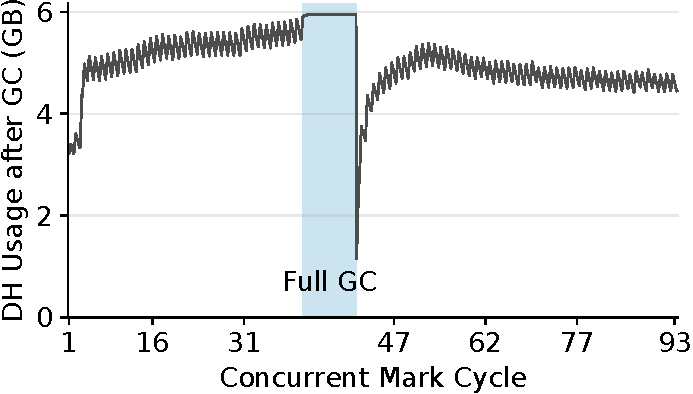
\includegraphics[width=0.325\linewidth]{chipper/figures/eval/model/g1_model_evac.pdf}}
	\subfloat[Space model]{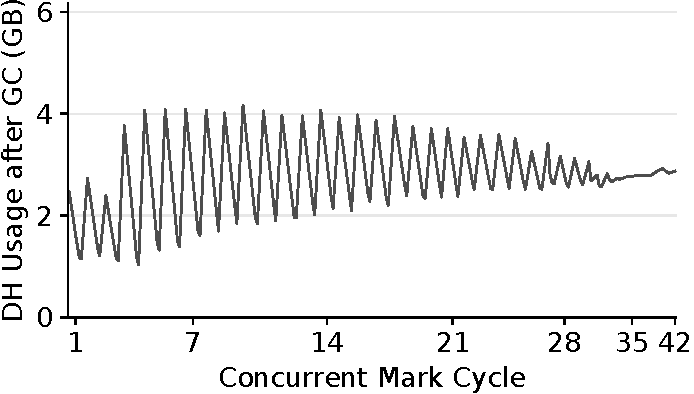
\includegraphics[width=0.325\linewidth]{chipper/figures/eval/model/space_model_evac.pdf}}
	\subfloat[\chipperName{} model]{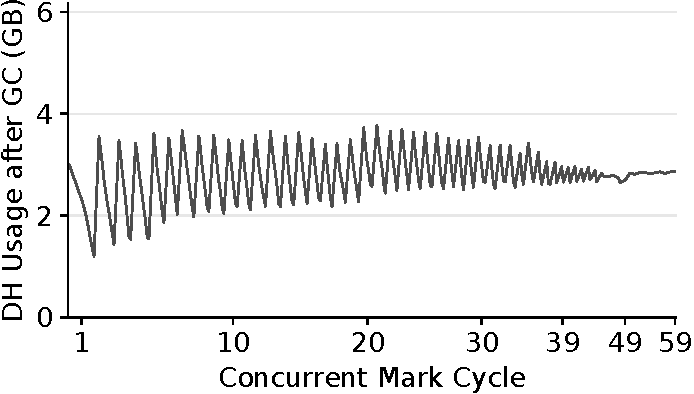
\includegraphics[width=0.325\linewidth]{chipper/figures/eval/model/cost_model_evac.pdf}}
	\caption{DH heap usage after Mixed and Full GCs for HBase Workload A under the three region-efficiency models used to rank candidate regions for collection.
		The x-axis denotes concurrent-mark cycles, each of which include multiple Mixed GCs.}
	\label{fig:model-heap}
\end{figure*}

Figure~\ref{fig:model-heap} shows why the G1 model triggers Full GCs.
Before the Full-GC sequence, Mixed GCs repeatedly collect regions but leave DH close to capacity.
The G1 model ranks regions using only the garbage reclaimed from the selected region and therefore does not account for the additional DH space reclaimed when live SH-candidate objects are moved to SH.
As a result, its Mixed GCs do not reclaim DH quickly enough to prevent memory pressure from reaching the Full-GC path.

The repeated Full GCs are amplified by G1's skip-compaction optimization.
During Full GC, G1 avoids compacting regions with less than 5\% garbage.
This optimization is normally useful because compacting nearly full regions provides little space benefit.
In this workload, however, some of these skipped regions contain live SH-candidate large objects.
Since large objects are migrated to SH through the Full-GC path, skipping these regions also postpones their migration.
Consequently, a Full GC can finish without reclaiming enough DH space, and another Full GC follows shortly afterwards.
For example, near the end of this sequence, one Full GC scans only 17 regions while skipping 1,355 regions.
The final Full GC instead scans 1,363 regions and skips only 9, allowing the remaining large SH candidates to be migrated.
The final Full GC migrates \SI{1.72}{GB} to SH, explaining the drop in DH usage in Figure~\ref{fig:model-heap}(a).

This large-object migration also explains the long Mixed GC pauses that follow.
The migrated large objects are subsequently updated by the application, creating backward references from SH to newly allocated objects in DH.
Before the final Full GC, the run has no backward references.
Immediately after the migration, the first Mixed GC processes 283,179 backward references and spends \SI{228.990}{ms} scanning the SH card table.
As execution continues, this cost becomes the dominant component of the longest Mixed GC pauses.
For the Mixed GC with the maximum pause, the collector processes 173,761 backward references and spends \SI{3021.291}{ms} scanning the SH card table.
This accounts for \SI{3021.291}{ms} of its \SI{3077.35}{ms} pause.
The Space and \chipperName{} models avoid this behavior because they reclaim sufficient DH space during Mixed GCs and therefore do not trigger the Full-GC migration of these large objects.
Their runs consequently have no backward references from these objects.

\begin{figure*}[h]
	% Legend
	
\includegraphics[width=.4\linewidth]{chipper/figures/eval/model/cost_model_evac_cycle13_legend.pdf}
	\\
	\subfloat[G1 model]{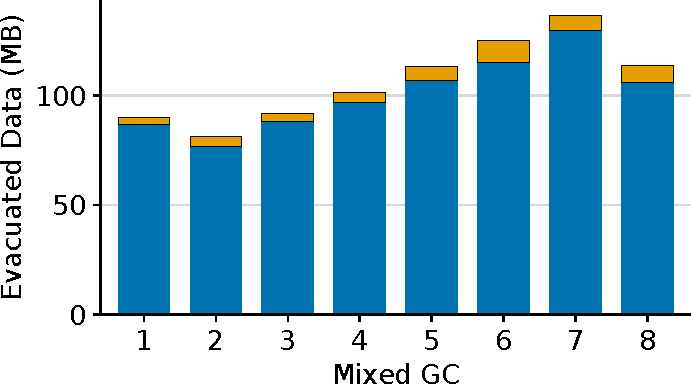
\includegraphics[width=0.325\linewidth]{chipper/figures/eval/model/g1_model_evac_cycle40.pdf}}
	\subfloat[Space model]{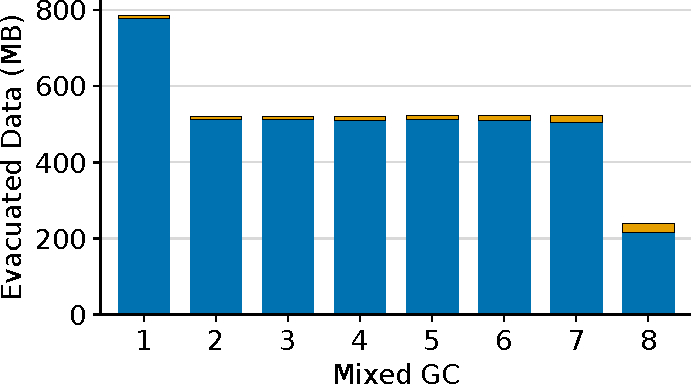
\includegraphics[width=0.325\linewidth]{chipper/figures/eval/model/space_model_evac_cycle4.pdf}}
	\subfloat[\chipperName{} model]{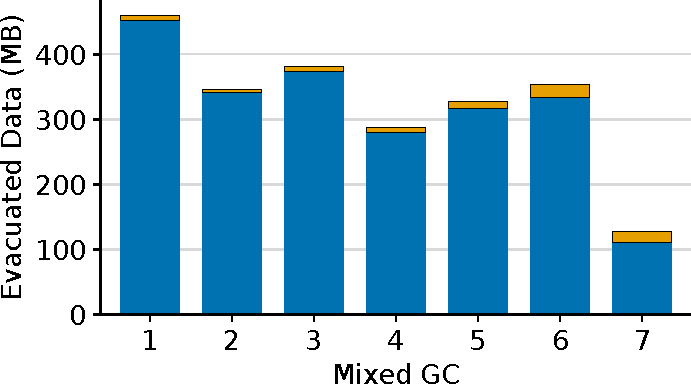
\includegraphics[width=0.325\linewidth]{chipper/figures/eval/model/cost_model_evac_cycle13.pdf}}
	\caption{Data evacuated to DH and SH by individual Mixed GCs within one concurrent-mark cycle for HBase Workload A under the three region-efficiency models, where (a) shows the G1 model in the concurrent-mark cycle immediately before the Full GC, (b) shows the Space model in the concurrent-mark cycle containing its maximum Mixed GC pause of \SI{1008.5}{ms}, and (c) shows the \chipperName{} model in the concurrent-mark cycle containing its maximum Mixed GC pause of \SI{521.87}{ms}.}
	\label{fig:model-evacuation}
\end{figure*}

Figure~\ref{fig:model-evacuation} isolates the remaining difference between the Space and \chipperName{} models.
For the G1 model, we show the concurrent-mark cycle immediately before the Full-GC sequence.
Its eight Mixed GCs evacuate only about \SI{806}{MB} to SH in total, which is insufficient to prevent DH from reaching the Full-GC path.
For the Space and \chipperName{} models, we show the concurrent-mark cycles containing their maximum Mixed GC pauses.
The Space model evacuates \SI{4055}{MB} to SH in this cycle, whereas \chipperName{} evacuates \SI{2207}{MB}, a difference of \SI{1848}{MB}.
The Space model credits SH-bound live bytes as reclaimed DH space but does not account for their higher SH evacuation cost.
It therefore assigns overly high efficiency to regions with large amounts of SH-bound live data and can place too much SH evacuation work in the same Mixed GC cycle.
The \chipperName{} model includes the SH evacuation cost in the region-efficiency calculation, reducing the amount of expensive SH evacuation selected together.
This difference reduces the maximum Mixed GC pause from \SI{1008.50}{ms} with the Space model to \SI{521.87}{ms} with \chipperName{}, while still reclaiming enough DH space to avoid Full GC.

\subsection{Impact of SH Allocation-Lock Granularity}
\label{sec:eval-scalability}

We evaluate how SH allocation-lock granularity affects Mixed GC performance and application tail latency.
As a baseline, we use a single global allocation lock, which serializes SH destination reservation and updates to the shared SH allocation metadata.
We compare this baseline with \chipperName{}'s per-region allocation locks, which allow GC threads targeting different SH regions to reserve destinations concurrently.

We evaluate all four applications, but report Lucene and Spark in Table~\ref{tab:allocation-locks} because they expose allocation-lock contention.
HBase and OpenSearch evacuate only a few thousand objects per Mixed GC, and these objects are relatively large.
They therefore perform fewer SH allocation operations and acquire the allocation lock less frequently.
As a result, the global and per-region implementations have similar Mixed GC pause distributions and application P99 latency for HBase and OpenSearch, so we omit them for brevity.

\begin{table*}[h]
	\centering
	\small
	\setlength{\tabcolsep}{3.5pt}
	\renewcommand{\arraystretch}{1.05}

	\caption{Impact of SH allocation-lock granularity on application P99 latency, Mixed GC time and pause distribution, and SH filler space overhead from duplicate evacuation reservations.}
	\label{tab:allocation-locks}

	\begin{tabular}{@{}cccccccccc@{}}
		\toprule

		\multirow[c]{2}{*}[-0.6ex]{\textbf{Application}}
		 &
		\multirow[c]{2}{*}{\textbf{\shortstack[c]{Lock      \\ granularity}}}
		 &
		\multirow[c]{2}{*}{\textbf{\shortstack[c]{P99 query \\ latency (ms)}}}
		 &
		\multicolumn{6}{c}{\textbf{Mixed GC}}
		 &
		\multirow[c]{2}{*}{\textbf{\shortstack[c]{Filler    \\space (\%)}}}
		\\

		\cmidrule(lr){4-9}

		 &
		 &
		 &
		\textbf{\#}
		 &
		\textbf{\shortstack[c]{Time                         \\(s)}}
		 &
		\textbf{\shortstack[c]{P50                          \\(ms)}}
		 &
		\textbf{\shortstack[c]{P95                          \\(ms)}}
		 &
		\textbf{\shortstack[c]{P99                          \\(ms)}}
		 &
		\textbf{\shortstack[c]{Max                          \\(ms)}}
		 &
		\\

		\midrule

		\multirow{2}{*}{Lucene}
		 & Global
		 & 5.5
		 & 83
		 & 5.8
		 & 64.89
		 & 140.35
		 & 206.64
		 & 227.41
		 & 0.00
		\\

		 & Per-region
		 & 1.7
		 & 15
		 & 1.1
		 & 69.10
		 & 124.26
		 & 166.27
		 & 166.29
		 & 0.20
		\\

		\midrule

		\multirow{2}{*}{Spark}
		 & Global
		 & 87
		 & 321
		 & 115.9
		 & 345.97
		 & 921.32
		 & 1022.48
		 & 1082.11
		 & 0.00
		\\

		 & Per-region
		 & 3.1
		 & 68
		 & 23
		 & 304.19
		 & 641.09
		 & 652.21
		 & 673.90
		 & 0.17
		\\

		\bottomrule
	\end{tabular}
\end{table*}


Table~\ref{tab:allocation-locks} shows that per-region locking substantially reduces Mixed GC time.
For Lucene, total Mixed GC time decreases from 5.8~s to 1.1~s, an 81\% reduction.
For Spark, it decreases from 115.9~s to 23.0~s, an 80\% reduction.
The number of Mixed GCs also decreases from 83 to 15 for Lucene and from 321 to 68 for Spark.

Per-region locking also reduces Mixed GC pause times, especially at the tail.
For Lucene, P50 increases slightly from 64.9~ms to 69.1~ms, while P95, P99, and the maximum pause decrease by 11\%, 20\%, and 27\%, respectively.
For Spark, P50, P95, P99, and the maximum pause decrease by 12\%, 30\%, 36\%, and 38\%, respectively.
These results show that the global lock limits evacuation parallelism when GC threads frequently reserve destinations in SH, whereas per-region locks allow reservations to proceed in parallel across different SH regions.

The reduction in Mixed GC time and pause times translates to lower application tail latency.
For Lucene, P99 query latency decreases from 5.5~ms to 1.7~ms, a 69\% reduction.
For Spark, P99 query latency decreases from 87.0~ms to 3.1~ms, a 96\% reduction.

Per-region locking introduces little additional SH space overhead from duplicate evacuation reservations.
SH filler objects occupy only 0.20\% of allocated SH space for Lucene and 0.17\% for Spark.
Thus, per-region allocation locks preserve parallel SH evacuation while adding negligible filler-space overhead.

\subsection{DH Space Reclaimed from Large Objects}
\label{sec:eval-large}

To evaluate the impact of placing large-object migration on the incremental-GC path, we compare two Lucene configurations.
In the first, we increase the G1 region size from its \SI{4}{MB} default for this heap size to \SI{16}{MB}, causing the large Lucene objects in this experiment to fall below G1's humongous-object threshold and therefore become eligible for regular evacuation to SH during Mixed GCs.
In the second, we use the default \SI{4}{MB} regions, under which these objects are humongous and \chipperName{} defers their migration to Full GC using the collector's existing mechanism for relieving memory pressure.
We use the larger region size as an experimental mechanism to place these objects on the Mixed GC evacuation path.

\begin{figure*}[h]
	\centering
	\subfloat[Query tail latency and throughput]{
		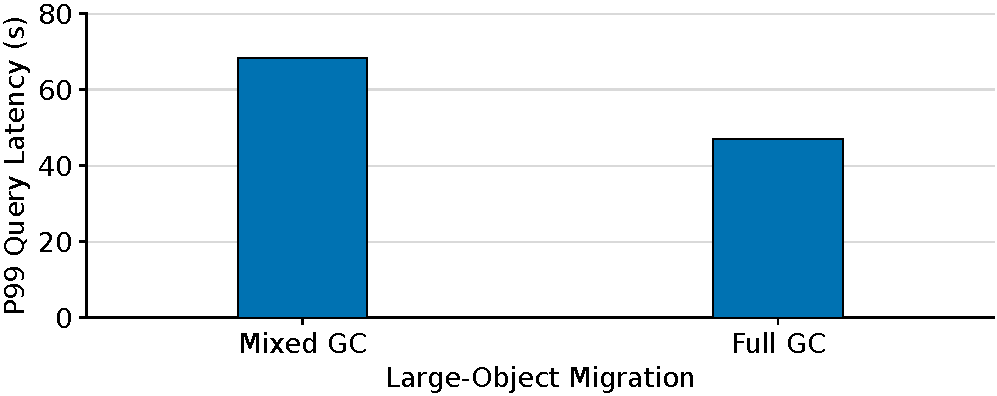
\includegraphics[width=0.48\linewidth]
		{chipper/figures/eval/humongous/lucene_large_object_performance.pdf}
	}
	\hfill
	\subfloat[Distribution of Mixed GC pauses]{
		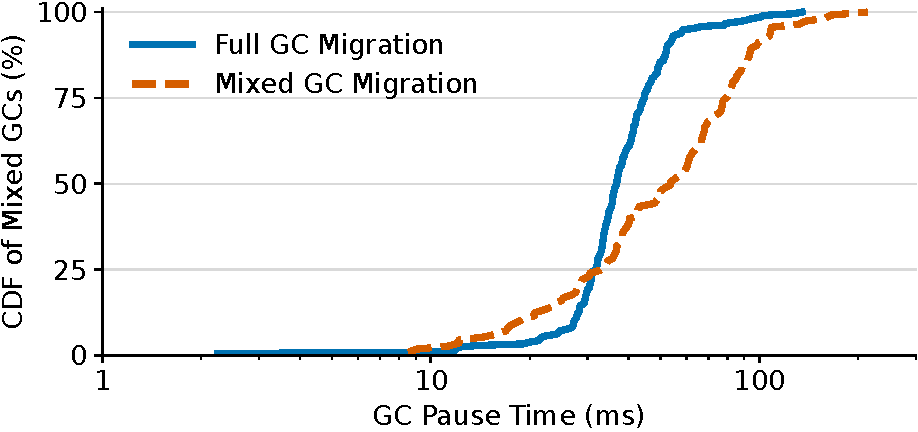
\includegraphics[width=0.48\linewidth]
		{chipper/figures/eval/humongous/gc_pauses_cdf.py.pdf}
	}

	\caption{
		Impact of large-object migration strategy on Lucene.
		(a) Achieved throughput and P99 query latency when large objects are migrated during Mixed GCs or Full GCs.
		(b) Distribution of Mixed GC pause times for the two migration strategies.	}
	\label{fig:humongous}

\end{figure*}

Figure~\ref{fig:humongous}(a) shows that deferring large-object migration to Full GC improves application performance.
At a target throughput of 200~ops/s, Full-GC migration achieves 182.68~ops/s, compared with 172.72~ops/s when large objects are migrated during Mixed GCs, a 5.8\% improvement.
Full-GC migration also reduces P99 query latency from 68.3~s to 47.0~s, a 31.2\% reduction.

Figure~\ref{fig:humongous}(b) explains this improvement.
Migrating large objects during Mixed GCs adds their copy cost to latency-critical incremental collections, shifting the Mixed GC pause distribution toward longer pauses and producing a heavier tail.
Deferring this work to Full GC removes large-object copying from the Mixed GC evacuation path, shifting the distribution toward shorter pauses.
Consequently, Mixed GCs perform only the regular evacuation work for which the incremental collector is designed, while large-object migration is performed on the less frequent memory-pressure-relief path.
The shorter Mixed GC pauses reduce interference with application execution, which leads to both higher achieved throughput and lower P99 query latency.

\section{Conclusion}

Latency-sensitive applications rely on both low-pause garbage collectors and large result caches to keep response times low.
Yet existing approaches cannot scale result caches beyond DRAM without introducing overheads that affect tail latency: storage-backed off-heap caches incur S/D costs, while prior storage-backed heaps rely on throughput-oriented collectors with long GC pauses.
We present \chipperName{}, the first storage-backed heap for low-pause garbage collectors.
\chipperName{} integrates migration to storage with the collector's GC work budget, preserves evacuation parallelism across SH regions, and provides a separate migration path for large objects that are not evacuated during incremental GCs.
We implement \chipperName{} in G1 and evaluate it with OpenSearch, Lucene, HBase, and Spark.
\chipperName{} improves P99 latency by up to $161\times$ over DRAM-limited on-heap caches, $34\times$ over storage-backed off-heap caches, and $9\times$ over TeraHeap.
These results show that fast local storage can extend managed heaps for latency-sensitive applications without sacrificing low-pause garbage collection.

\section*{Chapter Summary}
Latency-sensitive services running on the Java Virtual Machine (JVM) keep response times low with two mechanisms: low-pause garbage collection (GC), which collects the heap incrementally to bound pauses, and large result caches, which avoid recomputation.
These caches consume scarce DRAM and increase GC overhead, since cached objects stay reachable and the garbage collector must repeatedly scan them.
Placing them off-heap on fast storage relieves both, but introduces serialization and deserialization (S/D) on every access, raising latency.
Prior work avoids S/D cost and reduces GC scans with a storage-backed heap, but targets throughput-oriented collectors, whose long pauses are unsuitable for latency-sensitive services.

We present \chipperName{}, the first storage-backed heap for low-pause garbage collectors.
\chipperName{} extends the JVM with a second, high-capacity heap memory-mapped over an NVMe SSD, and migrates cache objects to it.
Migrated objects remain accessible as ordinary objects and are excluded from GC scans.
To preserve low latency, \chipperName{} (1) incorporates the cost of migration to the storage heap into the collector's cost model for incremental GCs, (2) integrates migration into the collector's parallel object-copying path, and (3) introduces a separate path for migrating objects that cannot be moved during incremental GCs.
We implement \chipperName{} in G1, the default garbage collector of OpenJDK, and evaluate it across four classes of latency-sensitive systems: search engines with OpenSearch, search libraries with Lucene as a foundation for many modern search engines, key-value stores with HBase, and stream-processing frameworks with Spark.
Our evaluation shows that \chipperName{} achieves up to $161\times$ lower P99 latency than DRAM-limited on-heap caches, $34\times$ lower than storage-backed off-heap caches, and $9\times$ lower than TeraHeap, a state-of-the-art storage-backed heap.


%

\setstretch{1.15}

\chapter{I/O-Aware Dynamic Heap Sizing}
\label{chapter:flexheap}

\section{Introduction}

Widely used search and analytics systems~\cite{elastic_search,lakshman:cassandra,mccandless:lucene,zaharia:spark} require substantial data movement to and from storage devices.
Such applications typically run on managed runtimes, particularly the Java Virtual Machine (JVM).
To mitigate the performance impact of I/O, these systems rely heavily on the OS page cache (I/O cache) in DRAM~\cite{apapag:aquila,apapag:fmap,jmal:hugemap,guanyu:tricache,huang:flashmap}, which buffers frequently accessed data to reduce access latency and I/O traffic.
However, dividing DRAM between the JVM heap and the I/O cache has become increasingly challenging as applications process larger datasets while DRAM capacity scaling slows down~\cite{damon,zombieland,tirmazi:borg,weiner:tmo}.
As a result, runtime adjustments to DRAM partitioning between the heap and the I/O cache can have a substantial impact on performance: allocating more memory to the heap can starve the I/O cache and increase I/O stalls, while allocating less increases garbage collection (GC) overhead~\cite{flexheap:jones:gc_handbook}.

Existing heap resizing mechanisms~\cite{sun:multi_space_heap,wang:elasticMem,boehm:gc,zgc:heap_resize} improve GC efficiency but remain agnostic to the interaction between GC and I/O performance.
They aim to reduce GC-related costs, such as pause time or GC CPU overhead, by adjusting heap size rather than managing the trade-off between heap and I/O cache usage.
For example, Garbage First (G1)~\cite{detlefs:g1}, the default OpenJDK collector, adjusts heap size based on GC behavior: it grows the heap to reduce GC frequency and releases memory when observed pauses stay below user thresholds.
To overcome the lack of I/O awareness, users often cap the maximum heap at a fixed fraction of DRAM, leaving the remainder to the I/O cache.
For instance, Cassandra~\cite{lakshman:cassandra} and Elasticsearch~\cite{elastic_search} recommend assigning about half of the memory to the heap and half to the I/O cache~\cite{elasticsearch:guidelines,cassandra:guidelines}.
The collector’s resizing mechanism still operates within these bounds.
However, the heap cannot grow beyond the cap even when application demand rises, increasing GC overhead during phases with high allocation rates that require more heap space (Section~\S\ref{sec:gc_driven}).

Previous work~\cite{jep351,jep346,wang:elasticMem,bruno:resize} has also examined how to reduce memory usage in containerized deployments by returning unused committed heap memory to the OS eagerly.
Vertical G1 (VG1)~\cite{bruno:resize,jep346} preserves G1’s heuristics and adds periodic triggers to uncommit memory to meet memory usage targets, but it does not incorporate I/O cost in its decisions.
Consequently, such occupancy-based resizing mechanisms fail to adapt during application phases where heap and I/O demands evolve together (Section~\S\ref{sec:occupancy_driven}).

In this work, we propose \flexheapName{}, the first heap resizing mechanism, to the best of our knowledge, that accounts for both GC and I/O overheads in dynamic memory partitioning.
We implement \flexheapName{} in G1, the default OpenJDK garbage collector, by replacing its heap resizing mechanism.
\flexheapName{} continuously monitors how GC and I/O stalls affect application performance and mitigates their impact by either growing the heap to reclaim memory from the I/O cache or shrinking it to release memory back to the I/O cache.
Our design tackles three key challenges:

\paragraph{\textbf{Estimating GC cost and I/O stalls}}
GC cost and I/O stalls manifest differently: GC includes stop-the-world (STW) pauses, where all application (mutator) threads are suspended, as well as concurrent phases, where GC threads run alongside mutators; I/O stalls occur when mutator threads block waiting for data from storage~\cite{kernel:sleeping}.
To estimate their impact, \flexheapName{} quantifies both costs in terms of lost compute cycles.
\flexheapName{} estimates CPU time differently for STW and concurrent phases of GC to reflect interference with mutator execution better.
To estimate the I/O stall of mutator threads, \flexheapName{} uses an Extended Berkeley Packet Filter (eBPF)~\cite{ebpf} program to track the time mutator threads spend in uninterruptible sleep~\cite{kernel:sleeping} state in the Linux kernel.

\paragraph{\textbf{Estimating the impact of heap resizing on GC cost and I/O stalls}}
GC cost and I/O stalls both depend on the amount of memory used by the respective operations.
However, an amount of memory may not necessarily have the same benefit for GC and I/O.
The relative effects of reassigning memory between the heap and the I/O cache depend on workload and system characteristics, such as access patterns, working-set size, and storage devices.
As a result, fixed weights for GC and I/O costs are difficult to choose, and a fixed analytical model of the GC--I/O relationship may not generalize across workloads and environments.
\flexheapName{} therefore adopts a model-free design and bases its resizing decisions by monitoring the cycles lost for performing GC and for I/O stalls.
When the combined cost increases, FlexHeap identifies which cost is responsible for this increase and guides subsequent resizing decisions.
In particular, FlexHeap considers as the dominant overhead not simply the largest component in absolute terms, but the one most sensitive to recent resizing decisions.

\paragraph{\textbf{Deciding the amount of the resizing step.}}
Resizing steps should be aggressive when the combined cost of GC and I/O stalls increases, and conservative near steady state.
In addition, shrink steps must respect G1’s pause time goal, which depends on maintaining enough eden space for the allocation of new objects.
\flexheapName{} sizes each step in two stages.
First, it computes a safe budget under G1 constraints: for growth, it limits the step to the available headroom below the maximum heap size, and for shrinking, it uses only the free space beyond the eden space required for the pause time goal.
Then, \flexheapName{} sizes the step according to how the total cost has changed in the last interval: larger increases trigger larger adjustments, small changes lead to small steps, and bounds prevent overshoot.

We implement \flexheapName{} in the G1 garbage collector of OpenJDK 21, a widely adopted long-term support release of the OpenJDK.
We evaluate \flexheapName{} using two widely used systems: Elasticsearch and the analytic framework Spark.
\flexheapName{} improves performance on average by 30\% for Elasticsearch and by 33\% for Spark.
Compared to VG1, \flexheapName{} achieves on average 50\% higher performance, showing that memory repartitioning must also account for I/O-induced stalls in such workloads.

Overall, our paper makes the following contributions:

\begin{itemize}
\item We examine the trade-off between application DRAM demands for heap and I/O cache and show the potential for improving overall performance by dynamically dividing DRAM between the two uses.

\item We propose an \emph{application-agnostic and adaptive} mechanism which reassigns memory between heap and I/O cache by considering the combined overhead of \flexheapGC{} and I/O stalls during execution.

\item We evaluate \flexheapName{} on widely used search and analytics systems and show that it outperforms prior GC-based and occupancy-based heap resizing mechanisms.

\end{itemize}

\section{Motivation}
\label{flexheap:sec:motiv}

We motivate the need for a dynamic heap-resizing mechanism that accounts for both \flexheapGC{} and I/O stalls.
Specifically, we show that existing heap-resizing mechanisms fail to adapt to the phase behavior of applications, whose heap and I/O cache demands vary over time.
To illustrate this limitation, we use Elasticsearch, a widely used production-grade search engine deployed at scale for log analytics, full-text search, and observability workloads.
We run the Wikipedia workload that performs concurrently search and document ingestion.
During ingestion, incoming documents are indexed and made searchable.
Section~\S~\ref{flexheap:sec:methodology} describes the full experimental setup.

\begin{figure*}[t]
	
\includegraphics[width=0.6\linewidth]{flexheap/fig/motiv/legend.pdf}
	\\
	\subfloat[G1-90]{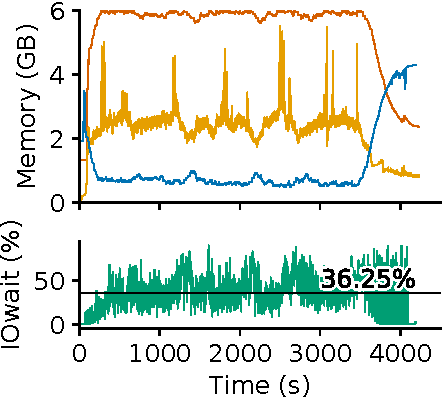
\includegraphics[width=0.245\linewidth]{flexheap/fig/motiv/nat90_ci4_cs32_d8g.pdf}}
	\subfloat[G1-50]{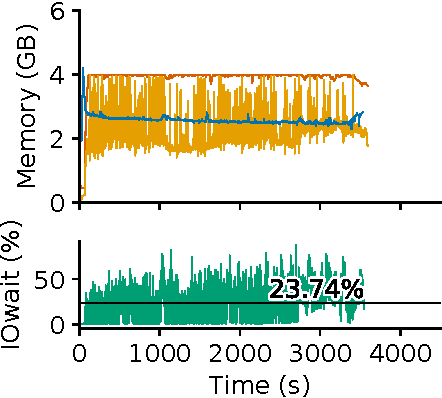
\includegraphics[width=0.245\linewidth]{flexheap/fig/motiv/nat50_ci4_cs32_d8g.pdf}}
	\subfloat[VG1]{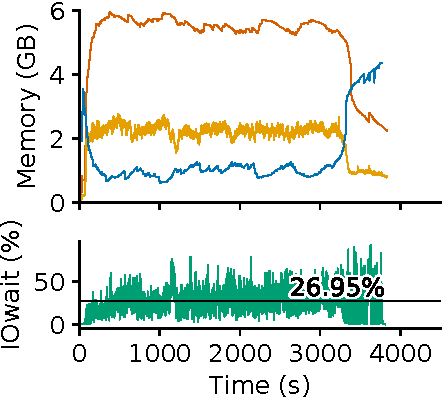
\includegraphics[width=0.245\linewidth]{flexheap/fig/motiv/je_ci4_cs32_d8g.pdf}}
	\subfloat[\flexheapName{}]{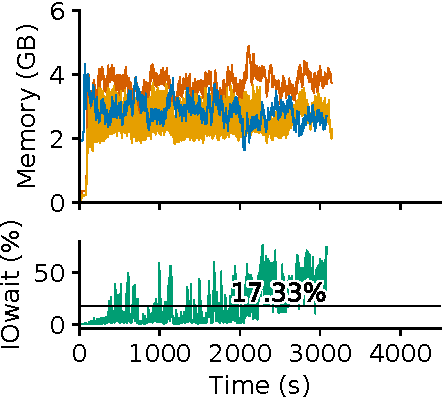
\includegraphics[width=0.245\linewidth]{flexheap/fig/motiv/fh_ci4_cs32_d8g.pdf}}
	\caption{
		Heap usage, I/O cache occupancy, and I/O wait over time for the Wikipedia workload in Elasticsearch:
		(a) G1-90 (with a maximum heap cap of 90\% of DRAM),
		(b) G1-50 (with a maximum heap cap of 50\% of DRAM),
		(c) VG1, and
		(d) \flexheapName{}.
	}
	\label{flexheap:fig:motiv}
\end{figure*}

\begin{figure}[t]
	
\includegraphics[width=0.4\linewidth]{flexheap/fig/motiv/xput_legend.pdf}
	\\
	\subfloat[Throughput]{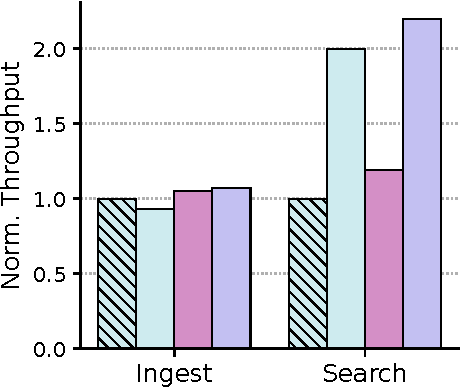
\includegraphics[width=0.3\linewidth]{flexheap/fig/motiv/xput.pdf}}
	\hspace{10pt}
	\subfloat[Latency]{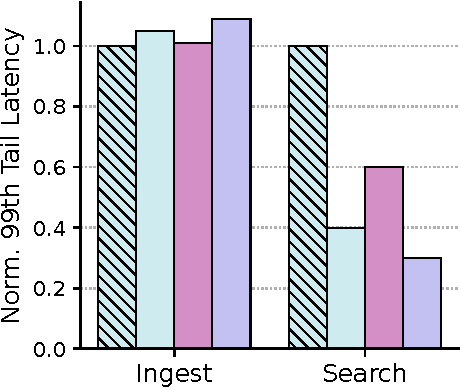
\includegraphics[width=0.3\linewidth]{flexheap/fig/motiv/lat.pdf}}
	\caption{Normalized document ingestion and query search (a) throughput, and
		(b) p99 latency for the Wikipedia workload in Elasticsearch under G1-90
		(with a maximum heap cap of 90\% of DRAM), G1-50 (with a maximum heap cap
		of 50\% of DRAM), VG1, and \flexheapName{}. Results are normalized to G1-90.}
	\label{fig:motiv:xput_lat}
\end{figure}

\subsection{GC-Based Heap Resizing Mechanisms Prioritize the Heap Over the I/O Cache}
\label{sec:gc_driven}

G1’s heap resizing mechanism cannot adapt to workloads that simultaneously stress the heap and the I/O cache because it relies solely on GC metrics.
In Figure~\ref{flexheap:fig:motiv}(a), we use G1 with the heap capped at 90\% of the available system DRAM (G1-90) on Elasticsearch running the Wikipedia workload.
Document ingestion and search run in parallel from the start until about \SI{3500}{s}, after which only search continues.
During this mixed phase, G1 continues to expand the committed heap until it reaches the configured cap.
Because its decisions consider only GC cost, G1 assigns nearly all available DRAM to the heap, leaving little space for the I/O cache; as a result, I/O wait remains high (about 36\% on average) for most of the execution.
After ingestion ends, heap usage drops to approximately \SI{1}{GB}, and the collector gradually returns memory to the OS; therefore, shrinking occurs only once heap pressure subsides.

Following Elasticsearch guidelines~\cite{elasticsearch:guidelines}, we cap the heap at 50\% of DRAM (G1-50) and run the same workload.
G1’s dynamic resizing remains active but is constrained by this cap.
Using G1-50, the execution time decreases by 15\% compared to G1-90.
This improvement is mainly due to the reduction of the average I/O wait by 24\% (a 33\% improvement over G1-90) because the I/O cache remains larger (approximately \SI{3}{GB}).
However, the cap restricts heap growth during document ingestion and consequently drives up GC activity: 54 full GCs instead of 1 in G1-90, plus 2{,}530 additional young and mixed GCs overall.
Under G1-50, document ingestion tasks run until the end of execution, resulting in 8\% lower document ingestion throughput compared to G1-90 (Figure~\ref{fig:motiv:xput_lat}(a)).
Conversely, the consistently larger I/O cache under G1-50 improves query performance: Figure~\ref{fig:motiv:xput_lat}(a) shows that search throughput is $2\times$ higher than under G1-90, and Figure~\ref{fig:motiv:xput_lat}(b) shows that p99 latency is 62\% lower.
This improvement primarily stems from a $2.4\times$ reduction in device read traffic compared to G1-90.

\subsection{Occupancy-Based Heap Resizing Mechanisms Ignore I/O Cost}
\label{sec:occupancy_driven}

Next, we examine whether time-driven, occupancy-based mechanisms, such as VG1, that return memory to the OS more aggressively can reduce I/O overhead.
As shown in Figure~\ref{flexheap:fig:motiv}(c), VG1 improves execution time by 5\% upon G1-90 but is insufficient without I/O awareness: during mixed phases, the heap remains near the cap and the I/O cache is constrained.
VG1 improves performance relative to G1-90 by reducing average I/O wait from 36\% to 27\% and increasing document ingestion throughput by 5\%.
However, it remains inferior compared to G1-50.
As VG1 does not adapt within the mixed ingestion–search phase, it continues to allocate most DRAM to the heap rather than the I/O cache when needed.
Consequently, Figure~\ref{fig:motiv:xput_lat}(a) shows that search throughput is approximately 40\% lower than G1-50, which maintains a larger I/O cache by capping the heap at 50\% of DRAM (at the cost of increased GC activity and lower document ingestion throughput).

\subsection{Considering Both GC and I/O Costs for Heap Resizing}

Figure~\ref{flexheap:fig:motiv}(d) shows \flexheapName{}, which resizes the heap using both \flexheapGC{} and I/O feedback.
During the mixed phase, it prevents the heap from monopolizing DRAM, leaving sufficient room for the I/O cache.
These results indicate that considering both \flexheapGC{} and I/O stalls enables more efficient DRAM use and higher end-to-end performance.
We present detailed results in the Section~\S\ref{flexheap:sec:eval}.

\section{\flexheapName{} Design}

\subsection{Overview}

The goal of \flexheapName{} is to improve application performance by effectively repartitioning memory between the heap and the I/O cache for applications that demand both.
We first outline how G1’s resizing mechanism currently works, then show how \flexheapName{} replaces it with a mechanism that considers both GC and I/O stalls.

% Achieving this is neither trivial: the JVM and the
% operating system make independent memory management decisions. The JVM resizes
% the heap to balance throughput and pause times, while the OS manages the page
% cache to reduce I/O latency. Because these two systems are unaware of each
% other’s state, improving one side often exponentially degrades the other,
% making coordinated resizing both necessary and challenging.
% To achieve such
% coordination, \flexheapName{} estimates the cost of \flexheapGC{} and I/O and dynamically
% repartitions DRAM between the heap and page cache to reduce the sum of both
% costs. \flexheapName{} operates entirely within the JVM, making on-the-fly decisions
% without requiring application-specific knowledge, as illustrated in
% Figure~\ref{fig:arch}.

Figure~\ref{fig:arch}(a) depicts G1’s heap resizing mechanism in OpenJDK 26.
Resizing criteria depend on the type of collection.
Young and mixed GCs occur more frequently than full GC, so they drive most resizing decisions.
In this path, heap resizing is based on the ratio of time spent in the GC versus the execution of mutator threads (GC time ratio).
If the GC time ratio consistently exceeds a threshold (\texttt{-XX:GCTimeRatio}), G1 decides to grow the heap.
If the ratio is consistently low, it decides to shrink the heap.
G1 uses a fraction of the uncommitted memory as the grow step, scaled based on the recent change in the GC time ratio.
The shrink step starts from the free committed bytes left after reserving the eden space target size, then scales that budget based on the recent change in the GC time ratio.
Then, based on the decision, G1 either commits additional memory or uncommits memory back to the OS.
On the other hand, after a full \flexheapGC{}, which is rare compared to young and mixed GCs, G1 compares the post GC free fraction to \texttt{ -XX:MinHeapFreeRatio} and \texttt{-XX:MaxHeapFreeRatio} and grows or shrinks the heap to keep free space within these bounds.
After heap resizing, G1 also sizes the eden space using a pause time model so that GC pauses meet the user-defined goal (\texttt{-XX:MaxGCPauseMillis}).

% G1 also determines the size of the eden space (Figure~\ref{fig:arch}(a)). This
% decision is key to balancing throughput and latency, as eden size directly
% impacts the number of allocations before the next GC. G1 uses a predictive
% model to estimate the pause time that would result from collecting a given
% number of eden regions, drawing on historical data such as evacuation cost per
% region, object copy time, and remembered-set processing overhead. If the
% estimated pause time exceeds the user-defined goal
% (\texttt{-XX:MaxGCPauseMillis}), G1 reduces the number of eden regions
% accordingly. This pause-time-driven sizing ensures that young GCs stay within
% latency targets while maximizing the interval between collections.

% Figure~\ref{fig:arch}(a) shows the heap resizing mechanism of G1 based on the
% latest version of OpenJDK (version 26). Heap resizing decisions follow
% different criteria depending on the type of collection. For young and mixed
% GCs, resizing is based on the ratio of time spent in GC versus application
% execution, known as the GC time ratio (\texttt{-XX:GCTimeRatio}). If recent
% \flexheapGC{} time ratios are high (e.g., the last four GCs or the average of the last
% ten exceed the threshold), G1 grows the heap to improve application throughput.
% To decide the amount of growing, G1 grows the heap by taking a fraction of the
% uncommitted memory scaling it by a bounded function of the GC-overhead delta.
% Conversely, if recent pause times are consistently low (e.g., the last eight
% consecutive GCs or the average of the last ten fall below a predefined
% threshold), G1 interprets this as low memory pressure and shrinks the heap. G1
% shrinks by taking the surplus free committed memory over the eden space target
% length, scaling that surplus by a bounded function of the GC-overhead delta.
% After a shrink, G1 uncommits the shrinked memory back to the OS.

% After a full GC (Figure~\ref{fig:arch}(a), G1 decides resizing based on the free
% fraction of the committed heap, compared against the two runtime thresholds
% (\texttt{-XX:MinHeapFreeRatio, -XX:MaxHeapFreeRatio}). It computes a minimum
% desired capacity that would leave at least MinHeapFreeRatio percent free space
% and a maximum desired capacity that would leave at most MaxHeapFreeRatio
% percent free space, bounded by the configured minimum and maximum heap sizes.
% If the committed capacity after the collection is below the minimum desired
% capacity, G1 grows the heap by the difference between those values. If it is
% above the maximum desired capacity, G1 shrinks the heap by that difference and
% uncommits memory back to the OS. Otherwise, the heap size remains unchanged.

\begin{figure}[t]
	\subfloat[G1]{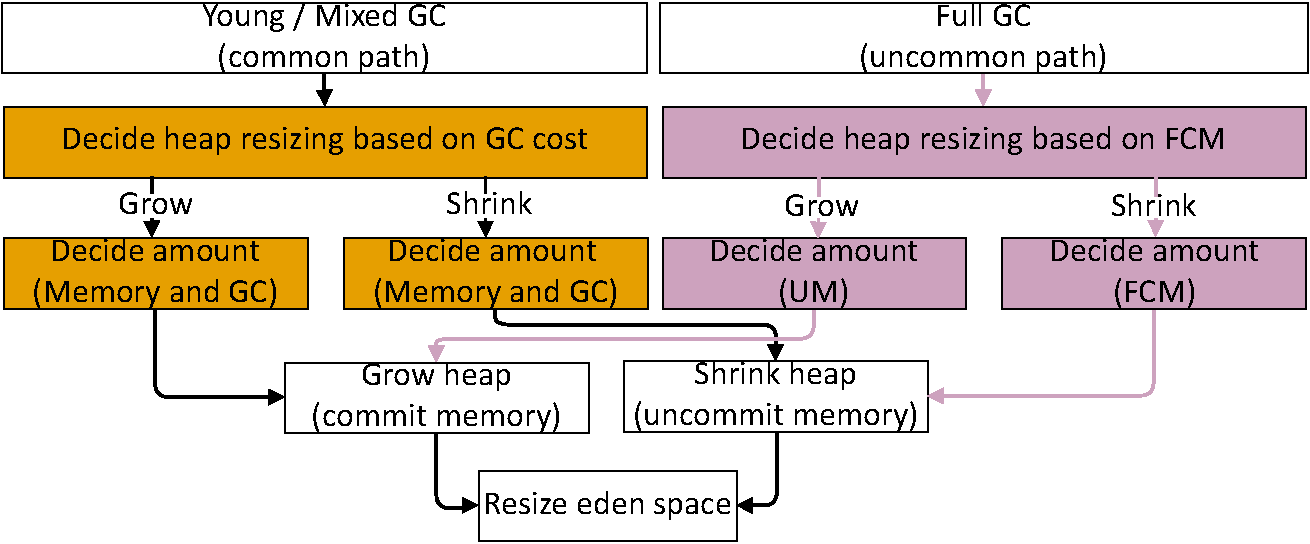
\includegraphics[width=0.56\linewidth]{flexheap/fig/design/g1_policy.pdf}}
	\subfloat[\flexheapName{}]{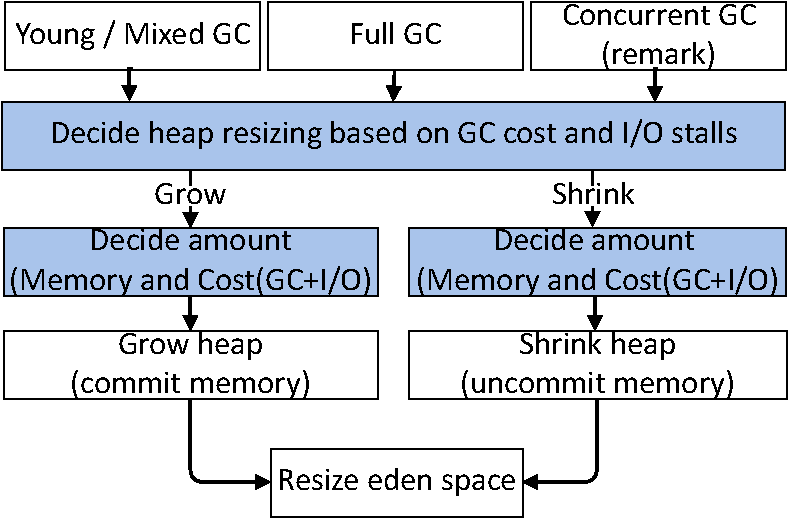
\includegraphics[width=0.355\linewidth]{flexheap/fig/design/fh_policy.pdf}}
	\caption{Overview of (a) G1 and (b) \flexheapName{} heap resizing mechanisms (acronyms:
		%
		\textbf{UM}=\textbf{U}ncommitted \textbf{M}emory,
		%
		\textbf{FCM}=\textbf{F}ree \textbf{C}ommitted \textbf{M}emory
	}
	\label{fig:arch}
\end{figure}

Figure~\ref{fig:arch}(b) illustrates the heap resizing mechanism of \flexheapName{} in G1.
We use a unified resizing mechanism regardless of the \flexheapGC{} type.
At each decision point, \flexheapName{}
%
(i) estimates the cost of GC (Section~\S~\ref{sec:gc_cost}) and I/O stalls (Section~\S~\ref{sec:io_cost}),
%
(ii) it uses the combined GC and I/O cost to grow or shrink the heap (Section~\S~\ref{sec:policy}), and
%
(iii) estimates the amount of memory to reassign (Section~\S~\ref{sec:resizing_step}).
%
Next, we discuss each mechanism of \flexheapName{} in more detail.

\subsection{Estimating Impact of \flexheapGC{}}
\label{sec:gc_cost}

\flexheapGC{} activity is the dominant overhead for heap operations.
We estimate the \flexheapGC{} CPU cycles spent in the current interval, defined as the time from the end of $\mathrm{STW}_{i-1}$ to the end of $\mathrm{STW}_{i}$.
Within this interval, we account for all \flexheapGC{} work: the concurrent \flexheapGC{} executed between pauses and the subsequent STW collection (young, mixed, or full GCs).
This concurrent activity includes the concurrent marking \flexheapGC{} cycle, and the work of concurrent refinement threads that update per-region remembered sets.
As the concurrent \flexheapGC{} overlaps with mutators, wall-clock time overestimates actual CPU usage.
Thus, we measure \flexheapGC{} cost in CPU time, following prior work~\cite{zgc:heap_resize}.
The total \flexheapGC{} CPU time of the current interval is the sum of CPU time spent in the subsequent STW \flexheapGC{}s and in concurrent \flexheapGC{}s:

\begin{align}
	\label{eq:gc_cost}
	\mathit{C}_\mathit{gc} = \mathit{C}_\mathit{stw} + \mathit{C}_\mathit{conc}
\end{align}

\paragraph{\textbf{STW GC CPU time}}
During an STW GC, all mutator threads are suspended, so the system loses the computation they could have performed during the pause time ($T_\mathit{stw}$).
The lost computation depends on the minimum of the available CPU cores ($N$) and the number of mutator threads ($M$).
The challenge is knowing $M$ at the pause boundary, as the mutator threads start and terminate over time, and some may already be waiting on locks.
\flexheapName{} therefore uses a practical upper bound: it maintains an atomic count of active Java mutator threads (excluding VM/GC/internal threads), incremented on thread start and decremented on termination, and reads this count at each STW boundary.
This may overestimate lost work because some counted threads could be non-runnable, but filtering them out would require a pre-safepoint runnability snapshot and per-transition instrumentation, adding prohibitive overhead.
Thus, we compute the STW cost as:

\begin{align}
	\label{eq:gc_stw}
	\mathit{C}_\mathit{stw} = T_\mathit{stw} \cdot \min(N, M)
\end{align}

\paragraph{\textbf{Concurrent GC CPU time}}
During concurrent \flexheapGC{}, both mutator and \flexheapGC{} threads execute in parallel and contend for CPU resources.
We estimate the portion of $G$ concurrent \flexheapGC{} threads that displace work from $M$ mutator threads, resulting in lost mutator progress.
$G$ includes both concurrent marking threads and refinement threads.
For this purpose, \flexheapName{} compares the total number of active threads ($M + G$) to the number of available cores $N$ for the specific interval.
When $M + G \leq N$, there are idle cores, and concurrent \flexheapGC{} can proceed without cost.
When $M + G > N$, some \flexheapGC{} threads preempt mutators, and only the excess CPU time beyond idle capacity contribute to overhead.
The concurrent cost is therefore:

\begin{align}
	\label{eq:conc_gc}
	\mathit{C}_\mathit{conc} =
	\begin{cases}
		\displaystyle \sum_{g \in G} T_{\mathrm{CPU}}(g) - \max\bigl(0,\,(N - M)\cdot T_\mathit{mut}\bigr), & M + G > N    \\
		0,                                                                                                  & M + G \leq N
	\end{cases}
\end{align}

Here, $T_\mathit{mut}$ is the time between the end of one STW phase and the start of the next, representing the interval during which mutator and concurrent GC threads overlap.
For example, on an 8-core system, suppose that during a given interval there are $M = 6$ mutators and $G = 4$ concurrent GC threads.
With $N = 8$, only $N - M = 2$ cores are available for concurrent GC, so $G - (N - M) = 2$ concurrent GC threads have no idle cores to run on; their CPU cycles in that interval are counted as overhead.
In addition to competing for cores, concurrent GC threads can also interfere with mutators through contention for other resources, such as cache and memory.
Precisely attributing that interference would require fine-grained hardware profiling which adds non-negligible overhead and complexity.

\subsection{Estimating Impact of I/O Stalls}
\label{sec:io_cost}
The memory available to the I/O cache directly determines how much time mutator threads spend stalled on I/O.
A larger I/O cache allows more frequently accessed data to be served from DRAM, reducing page faults that cause storage access and keeping mutators from getting context switched.
However, this benefit depends on the access locality: workloads with little or no reuse derive limited advantage from additional cache space.
Conversely, when the I/O cache is small or under pressure, a larger fraction of reads and writes must be served from the storage device, causing mutator threads to block in the kernel I/O path until the data are fetched into memory.
These stalls translate directly into CPU time that could otherwise be used for application processing, reducing performance.
To capture this effect, \flexheapName{} estimates the CPU time lost due to I/O stalls, using it as a measure of the performance cost of limited I/O cache space to guide resizing decisions.

\begin{algorithm}
	\caption{eBPF Handler for \texttt{sched\_switch}.}
	\begin{algorithmic}[1]
		\Procedure{on\_sched\_switch}{prev\_tid, next\_tid, prev\_state}
		\State ts $\gets$ current\_time()

		\If {prev\_tid $\in$ mutators \textbf{and} prev\_state = D}
		\State iostart[prev\_tid] $\gets$ ts
		\EndIf

		\If {next\_tid $\in$ mutators \textbf{and} next\_tid $\in$ iostart}
		\State dt $\gets$ ts $-$ iostart[next\_tid]
		\If{next\_tid $\in$ iowait}
		\State iowait[next\_tid] $\gets$ iowait[next\_tid] $+$ dt
		\Else
		\State iowait[next\_tid] $\gets$ dt
		\EndIf
		\State \textbf{delete} iostart[next\_tid]
		\EndIf
		\EndProcedure
	\end{algorithmic}
	\label{alg:ebpf}
\end{algorithm}

To quantify this loss, we measure the time mutator threads spend in the uninterruptible (D) state~\cite{kernel:sleeping}, during which they are blocked on I/O and cannot make progress.
Even when other threads continue to use the CPUs, these stalled mutators still represent lost opportunities for mutator progress.
$C_\mathit{io}$ therefore captures mutator progress lost while threads are blocked on I/O.
This differs from $C_\mathit{gc}$, which estimates the loss caused by \flexheapGC{} displacing runnable mutators from the CPU.
Measuring $C_\mathit{io}$ only as idle-core-equivalent stall time would therefore underestimate the impact of I/O-bound phases, particularly in services where blocked mutators contribute to queue buildup and tail latency.

% \flexheapName{} requires a per-mutator-thread approximation of I/O stall time, which
% standard kernel interfaces do not directly expose. The \texttt{iowait} metric in
% \texttt{/proc/stat} is insufficient for this purpose because it is a CPU-level
% aggregate metric: it indicates that a CPU is idle while at least one task is
% waiting for I/O~\cite{linux:iowait}, rather than the stall time of a specific
% thread. Thus, a mutator may be blocked on a lock while an unrelated task on the
% same CPU waits for I/O, making \texttt{iowait} an incorrect proxy for the
% mutator's I/O stall time. More fundamentally,

Existing standard kernel interfaces do not directly expose the time per mutator thread lost to I/O stalls.
The \texttt{iowait} metric in \texttt{/proc/stat} is a CPU-level aggregate metric.
It reports that a CPU is idle while at least one task is waiting for I/O~\cite{linux:iowait}, rather than how much time a particular thread is stalled on I/O.
For example, a mutator thread may be blocked on a lock while an unrelated thread on the same CPU waits for I/O, so treating the recorded \texttt{iowait} as the mutator's I/O stall time would be incorrect.
More fundamentally, kernel interfaces do not directly expose per-thread I/O stall measurements, because scheduler semantics decouple I/O completion from rescheduling.
For example, a thread's I/O may complete before the scheduler places the thread back on a CPU, making it unclear whether the intervening delay should be counted as I/O stall time.

\flexheapName{} implements an eBPF~\cite{ebpf} program attached to the \texttt{sched\_switch} tracepoint to obtain an approximation of the per mutator thread I/O stall time, as shown in Algorithm~\ref{alg:ebpf}.
The eBPF program maintains two maps: \texttt{iostart}, which stores the timestamp at which a mutator thread enters the D state, and \texttt{iowait}, which accumulates the total time that the thread has spent blocked on I/O.
On each context switch, if a tracked mutator thread is scheduled out in the D state, we record the current timestamp in \texttt{iostart}; when it is scheduled back in, we compute the elapsed time since that timestamp and add it to \texttt{iowait}.
We use the accumulated value in \texttt{iowait} as the mutator CPU time lost to I/O stalls.

To ensure the estimate respects hardware limits, the computed I/O-induced CPU time loss must not exceed the machine’s compute capacity over the measurement interval.
When the number of mutator threads exceeds the available CPU cores and all are simultaneously stalled on I/O, the total lost CPU time cannot be greater than the interval duration multiplied by the number of cores.
We therefore cap the measured stall time to the product of the interval duration and the number of CPU cores, as shown in Eq.~\ref{eq:io}:

\begin{equation}
	\label{eq:io}
	\mathit{C}_\mathit{io} = \min \bigl(\displaystyle \sum_{m \in M} T_{\mathrm{io}}(m), T_\mathit{mut} \cdot N \bigr)
\end{equation}

\subsection{Deciding to Grow or Shrink the Heap}
\label{sec:policy}

% FlexHeap uses a feedback-driven, model-free controller because the relationship
% between heap size, GC overhead, and I/O-cache benefit is highly sensitive to
% the workload phase and system environment. In particular, shrinking the heap
% does not imply a fixed or proportional reduction in I/O cost: the resulting
% benefit depends on the application's access pattern, working-set size, storage
% characteristics, and whether the memory released from the heap is actually
% available to and beneficial for the page cache. While a model-based design
% could potentially adapt faster when its assumptions hold, FlexHeap instead
% prioritizes robustness across workloads and storage environments by reacting to
% observed changes in GC and I/O cost.

After each \flexheapGC{} cycle, \flexheapName{} determines whether to grow the heap (\texttt{growHeap}) or shrink the heap (\texttt{shrinkHeap}) to release memory for the I/O cache.
For the decision-making process, \flexheapName{} compares, across intervals, the sum of CPU time consumed by \flexheapGC{} and I/O stalls, which together capture lost mutator progress.
To reduce short-term noise, \flexheapName{} averages the sum of $C_\mathit{gc}$ and $C_\mathit{io}$ over the last ten intervals, following G1's use of a ten-interval moving average.
An alternative approach would be to balance these two costs, aiming for equal contribution from both.
However, this does not necessarily minimize total overhead.
Equalizing the two costs may still yield suboptimal performance.
For example, in scan-heavy workloads with low I/O cache hit rates, prioritizing I/O cost could enlarge the I/O cache without improving throughput, while simultaneously inflating \flexheapGC{} overhead.
This counterproductive behavior shows that balancing costs is insufficient—\flexheapName{} instead seeks to reduce their combined sum.

% Summing these two costs has two benefits. First, it directly reduces total
% overhead, whereas balancing \flexheapGC{} and I/O stall costs does not necessarily
% reduce end-to-end performance loss. For example, in scan-heavy workloads with
% low I/O-cache hit rates, prioritizing I/O cost could enlarge the I/O cache
% without improving throughput, while simultaneously increasing \flexheapGC{} overhead.
% Second, it avoids introducing explicit weights for each cost. A weighted
% formulation would require tuning the relative importance of heap-related and
% cache-related effects, which may vary across workloads and execution phases.

If a \texttt{shrinkHeap} (or \texttt{growHeap}) action reduces the total cost ($C_\mathit{tot} = C_\mathit{gc} + C_\mathit{io}$), \flexheapName{} continues applying the same action.
However, whenever \flexheapName{} applies a resize action, it must account for the delay before the effects of the previous resize are reflected in heap usage or I/O cache growth.
Without waiting for the repurposed memory to be absorbed by the heap or the I/O cache, \flexheapName{} could issue premature actions, resulting in unnecessary or even harmful resizing.
This is particularly important when memory released from the heap does not improve the I/O cache, for example because the application uses direct I/O, or because, in a multitenant container, the freed memory is consumed by sibling processes instead.

\begin{figure}[t]
	\centering

	\begin{minipage}{\linewidth}
		\centering
		\resizebox{0.65\linewidth}{!}{%
			\begin{tabular}{ccc}
				\toprule
				\textbf{Predicate}                                                              &
				\textbf{Predicate Definition}                                                   &
				\textbf{Complementary Predicate}                                                  \\
				\midrule
				\texttt{costDown}                                                               &
				$C_\mathrm{tot}[t] \leq C_\mathrm{tot}[t-1]$                                    &
				\texttt{costUp}                                                                   \\
				\texttt{growSlack}                                                              &
				$S_\mathrm{used} < S_\mathrm{used\_before\_grow} + S_\mathrm{grow}$             &
				\texttt{growUsed}                                                                 \\
				\texttt{ioSlack}                                                                &
				$S_\mathrm{io} < S_\mathrm{io\_before\_shrink} + S_\mathrm{shrink}$             &
				\texttt{ioFull}                                                                   \\
				\texttt{gcBias}                                                                 &
				$\Delta^\mathrm{rel} C_\mathrm{gc}[t] \ge \Delta^\mathrm{rel} C_\mathrm{io}[t]$ &
				\texttt{ioBias}                                                                   \\
				\bottomrule
			\end{tabular}%
		}
	\end{minipage}

	\vspace{0.8em}

	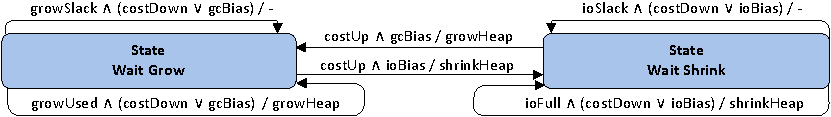
\includegraphics[width=\linewidth]{flexheap/fig/design/fh_logic.pdf}
	\caption{Finite-state machine of the FlexHeap resizing controller.
Each transition label has the form \textit{condition} / \textit{action}.
The table defines the predicates used in transition guards, their formal definitions, and the complementary predicate names.
For example, \texttt{growUsed} is the complement of \texttt{growSlack} and denotes the case where the heap has exhausted the space added by the previous grow step.
In the table, for the definition of predicates, $S$ denotes a size-related quantity.}
	\label{fig:fsm}
\end{figure}

To handle delayed effects, \flexheapName{} employs \emph{wait states}, which defer further resizing until the impact of the previous action becomes observable, as shown in Figure~\ref{fig:fsm}.
After a \texttt{growHeap} action, \flexheapName{} enters in the state \emph{Wait Grow}.
If $C_\mathit{tot}$ decreases and the space added by the previous grow step has not yet been exhausted (\texttt{growSlack}), the controller waits; if that space has been exhausted (\texttt{growUsed}), it issues another \texttt{growHeap} action.
Symmetrically, after a \texttt{shrinkHeap} action, \flexheapName{} enters in the state \emph{Wait Shrink}.
If $C_\mathit{tot}$ decreases and the memory released by the previous shrink step has not yet been fully consumed by the I/O cache (\texttt{ioSlack}), the controller waits; otherwise, it issues another \texttt{shrinkHeap} action.

Conversely, if $C_\mathit{tot}$ increases, \flexheapName{} determines the next direction by comparing the relative change of the two cost components, denoted by $\Delta^{\mathrm{rel}} C_x[t] = (C_x[t] - C_x[t-1]) / C_x[t-1]$.
If the relative change in $C_\mathrm{gc}$ is greater than or equal to that in $C_\mathrm{io}$ (\texttt{gcBias}), the controller infers that GC was affected more adversely by the last resizing step and issues \texttt{growHeap}; otherwise, it issues \texttt{shrinkHeap}.
We use relative rather than absolute changes because $C_\mathrm{gc}$ and $C_\mathrm{io}$ may differ by orders of magnitude and their dominance may shift across workloads and phases.
Comparing absolute values would bias the controller toward whichever component is currently larger, even when the other is more sensitive to heap resizing.
By normalizing each cost to its previous value, \flexheapName{} makes scale-invariant decisions based on which component changed more sharply in response to the last action.

A simpler alternative would be to immediately undo the previous resizing action whenever $C_\mathit{tot}$ increases.
We do not adopt this policy because such an immediate reversal may be premature and can induce oscillation.
$C_\mathit{gc}$ and $C_\mathit{io}$ respond differently to memory reassignment: additional heap memory generally reduces GC pressure, whereas releasing memory to the I/O cache does not always reduce I/O cost, depending on the workload’s working-set size and access pattern.

\paragraph{\textbf{Proactive GC triggering during mutator I/O stalls}}
Mutator threads can become blocked on I/O for an extended period, significantly delaying the next GC cycle.
When this happens, heap resizing decisions are also delayed, leading to feedback lag.
To maintain responsiveness in these cases, \flexheapName{} triggers a GC proactively when mutator threads stall as follows.

A lightweight VM thread runs periodically every second (similar to VG1) and monitors two runtime metrics: allocation rate and mutator I/O stall time.
\flexheapName{} samples the total bytes allocated by mutator threads every second.
It maintains a sliding window of recent allocation measurements and computes a moving average over the last five intervals.
If the current allocation rate drops by half, \flexheapName{} marks the interval as a low-activity period.
To avoid reacting to transient changes, it tracks how many of the last few intervals have shown low activity.
Only if multiple consecutive samples indicate reduced allocation rate, does it consider the system to be stalled.
For this period, \flexheapName{} also monitors I/O stall cycles.
If high stall time coincides with low allocation activity, \flexheapName{} concludes that threads are waiting on I/O rather than idle, and triggers a GC.
To avoid disrupting normal GC scheduling, \flexheapName{} inserts the GC request through standard internal JVM hooks, and ensures that no GC is already in progress.

\subsection{Estimating the Resizing Step}
\label{sec:resizing_step}

The goal of the growing and shrinking steps is to respond quickly to changes in application behavior and to respect G1’s pause time goals.
For responsiveness, \flexheapName{} scales each resize step by the recent change in the combined cost.
For pause protection, \flexheapName{} relies on G1’s eden sizing model and leaves it unchanged.
This model is not part of our resizing mechanism.
After each young or mixed \flexheapGC{}s, G1 measures the pause overhead.
It uses this metric to predict the next young-GC pause and then chooses the largest size for eden space that meets the user pause target within available free memory.
We use this model only to bound shrinking: the shrink step returns memory only from free regions beyond the computed target size of eden space.
Similar to G1’s resizing mechanism, we do not use the pause-time model for the growth step.
Growing only adds free regions, and G1’s eden sizing model still selects exactly as many eden regions as needed to meet the pause target.
Growth therefore follows G1’s bounded expansion mechanism, scaled by our total cost metric, while remaining aligned to region size and limited by uncommitted headroom.

\begin{figure}[h]
	\centering
	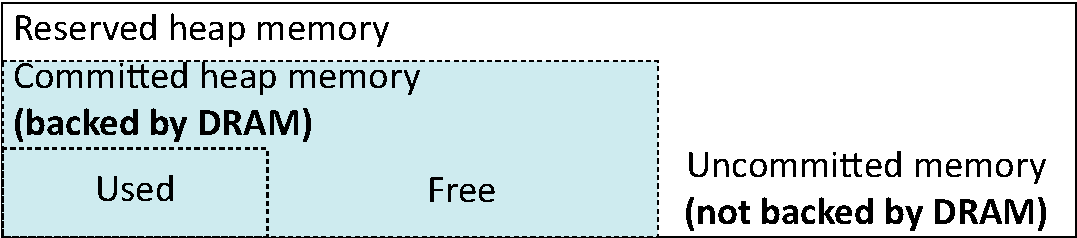
\includegraphics[width=0.5\linewidth]{flexheap/fig/design/jvm_mem.pdf}
	\caption{Committed and uncommitted heap memory.}
	\label{fig:jvm_mem}
\end{figure}

\begin{algorithm}[h]
	\caption{Growing step}
	\label{alg:growth_step}
	\begin{algorithmic}[1]
		\Procedure{grow\_amount}{$\Delta C_{\text{tot}}$}
		\State \texttt{reserved} \(\gets\) \texttt{max\_capacity}()
		\State \texttt{committed} \(\gets\) \texttt{capacity}()
		\State \texttt{uncommitted} \(\gets\) \texttt{reserved} \(-\) \texttt{committed}
		\State \texttt{expand\_via\_pct} \(\gets\) \texttt{G1ExpandByPercentOfAvailable} \(\times\) \texttt{uncommitted}
		\State \texttt{min\_expand} \(\gets \min(\texttt{RegionSize},\ \texttt{uncommitted})\)
		\State \texttt{resize\_bytes} \(\gets \min(\texttt{expand\_via\_pct},\ \texttt{committed})\) \label{line:resize}
		\State \texttt{scale\_factor} \(\gets\) \texttt{scale\_total\_cost\_delta}(\(\Delta C_{\text{tot}}\), \texttt{MinScaleFactor}, \texttt{MaxScaleFactor}) \label{line:scale}
		\State \texttt{resize\_bytes} \(\gets \texttt{resize\_bytes} \times \texttt{scale\_factor} \)
		\State \textbf{return} \(\max\!\big(\min(\texttt{resize\_bytes}, \texttt{uncommitted}), \texttt{min\_expand}\big)\)
		\EndProcedure
	\end{algorithmic}
\end{algorithm}

\paragraph{\textbf{Growing step}}
As shown in Figure~\ref{fig:jvm_mem}, the heap has committed memory (backed) and uncommitted memory (reserved up to maximum heap size).
A grow step, calculated by Algorithm~\ref{alg:growth_step}, cannot exceed the uncommitted headroom.
\flexheapName{} forms a base budget as the smaller of (i) a fixed percentage of the uncommitted headroom (the same percentage used by native G1) and (ii) the current committed size (Line~\ref{line:resize}).
This avoids oversized jumps that would reduce \flexheapGC{} frequency and risk longer pauses.
\flexheapName{} then scales the normalized cost change $\Delta C_{\text{tot}}$ using a step scale with a logistic (S-shaped) function (Line~\ref{line:scale}).
$\Delta C_{\text{tot}}$ is the change between intervals: larger increases yield larger steps, small changes yield conservative steps.
We adopt the same logistic form used by G1’s resizing mechanism, keeping tuning behavior consistent.
Finally, \flexheapName{} returns the grow bytes constrained to the admissible range.
The resize amount does not exceed the available uncommitted headroom and is not less than the minimum expansion.

\paragraph{\textbf{Shrinking step}}
Algorithm~\ref{alg:shrink_step} describes the computation for the shrink step.
We first use G1’s pause-time model to compute the number of regions needed to meet the eden target length (Line~\ref{line:eden}).
Then, we subtract it from the current number of free regions to obtain the shrinkable budget (Line~\ref{line:free}).
This respects G1’s pause time goal by not reducing eden below the target G1 selects.
We then ,similar to growing step, we scales the normalized cost change $\Delta C_{\text{tot}}$ using a step scale with a logistic (S-shaped) function (Line~\ref{line:scale2}).
Finally, we convert the shrinkable regions to bytes, and multiply by the scale factor to obtain the shrink amount.

\begin{algorithm}[h]
	\caption{Shrinking step}
	\label{alg:shrink_step}
	\begin{algorithmic}[1]
		\Procedure{shrink\_amount}{$\Delta C_{\text{tot}}$}
		\State \texttt{regions\_to\_shrink} \(\gets\) \texttt{num\_free\_regions}()
		\State \texttt{regions\_for\_eden\_space} \(\gets\) \texttt{eden\_target\_length}() \label{line:eden}
		\State \texttt{regions\_to\_shrink} \(\mathrel{-}= \texttt{regions\_for\_eden\_space}\) \label{line:free}
		\State \texttt{scale\_factor} \(\gets\) \texttt{scale\_total\_cost\_delta}(\(\Delta C_{\text{tot}}\), \texttt{MinScaleFactor}, \texttt{MaxScaleFactor}) \label{line:scale2}
		\State \texttt{resize\_bytes} \(\gets \texttt{regions\_to\_shrink} \cdot \texttt{RegionSize} \cdot \texttt{scale\_factor}\)
		\State \textbf{return} \(\texttt{resize\_bytes}\)
		\EndProcedure
	\end{algorithmic}
\end{algorithm}

% An interesting direction for future work is to augment the resizing step with a
% different model that estimates how much memory should be reallocated to the
% heap or to the I/O cache by capturing how useful additional memory is in each
% case. Such a model could also incorporate weights that reflect the relative
% importance of GC cost and I/O stalls.

\section{Methodology}
\label{flexheap:sec:methodology}

Our evaluation focuses on four questions:

\begin{enumerate}
\item How much does \flexheapName{} improve application performance for I/O intensive applications?

\item How do \flexheapName{}’s resizing decisions affect the tail latency?

\item How sensitive is \flexheapName{} to the (a) application phase changes, (b) storage device latency, and (c) resizing step?

\end{enumerate}

For this purpose, we use the following methodology, applications and benchmarks.

\paragraph{\textbf{Experimental platform.}}
We use a single server equipped with two Intel(R) Xeon(R) CPU E5-2630 running at \SI{2.4}{GHz}, with 16 physical cores with two threads per core.
It has \SI{256}{GB} of DDR4 DRAM and runs Ubuntu 20.04 with Linux kernel 5.4.
The server has one \SI{2}{TB} Samsung PCIe NVMe SSD and two \SI{256}{GB} Samsung 850 SATA SSD.
Unless otherwise stated, all experiments use the NVMe SSD.
The SATA SSDs are used only in the experiment that studies the impact of higher-latency storage devices.
To reduce variability, we disable swap and set the CPU scaling governor to \emph{performance}.
When necessary for each experiment, we limit the available DRAM capacity using \emph{cgroups}.
We run all experiments on OpenJDK 21, since it is the latest long-term-support version supported by both Elasticsearch and Spark.

\begin{table}[t]
	\centering
	\caption{Configurations of Elasticsearch workloads for each DRAM budget.
		G1-50 (G1 default heap resizing policy with maximum heap capped at 50\% of
		DRAM), VG1 (Vertical G1), and FH (\flexheapName{}) indicate the heap size allocated
		to each setup under the given DRAM budget.}
	\label{tab:es}
	\resizebox{\columnwidth}{!}{%
		\begin{tabular}{lrr cccc cccc}
			\toprule
			\multirow{2}{*}{\textbf{Dataset}} & \multirow{2}{*}{\textbf{Index (GB)}}         & \multirow{2}{*}{\textbf{\#Documents}}
			                                  & \multicolumn{4}{c}{\textbf{Configuration A}}
			                                  & \multicolumn{4}{c}{\textbf{Configuration B}}                                                                                                       \\
			\cmidrule(lr){4-7} \cmidrule(lr){8-11}
			                                  &                                              &
			                                  & \textbf{DRAM}                                & \textbf{G1-50}                        & \textbf{VG1}  & \textbf{FH}
			                                  & \textbf{DRAM}                                & \textbf{G1-50}                        & \textbf{VG1}  & \textbf{FH}                                 \\
			                                  &                                              &
			                                  & \textbf{(GB)}                                & \textbf{(GB)}                         & \textbf{(GB)} & \textbf{(GB)}
			                                  & \textbf{(GB)}                                & \textbf{(GB)}                         & \textbf{(GB)} & \textbf{(GB)}                               \\
			\midrule
			Wikipedia                         & 68                                           & 22,986,169                            & 8             & 4             & 7  & 7  & 12 & 6  & 11 & 11 \\
			Cohere Vector                     & 500                                          & 30,000,000                            & 25            & 13            & 22 & 22 & 50 & 25 & 45 & 45 \\
			Dense Vector                      & 19.5                                         & 10,000,000                            & 4             & 2             & 3  & 3  & 6  & 3  & 5  & 5  \\
			OpenAI Vector                     & 109.1                                        & 5,361,922                             & 4             & 2             & 3  & 3  & 7  & 3  & 6  & 6  \\
			\bottomrule
		\end{tabular}
	}
\end{table}


\paragraph{\textbf{Elasticsearch}}
We use Elasticsearch version 9.1.1, a widely deployed search engine, and evaluate it using the ESRally benchmarking suite~\cite{esrally}.
%
Our evaluation focuses on mixed workloads that perform concurrently search and document ingestion.
This concurrency creates time-varying demands for heap and I/O cache that do not form distinct execution phases.
%
ESRally runs on a separate server to avoid interference with Elasticsearch.
Each experiment is repeated five times, and we report average throughput and 99th-percentile tail latency.
%
ESRally measures ingestion throughput in documents per second, while search throughput is measured in queries per second.
%
The Elasticsearch server is configured to use all CPU cores.
We let the JVM ergonomics automatically choose the number of STW and concurrent GC threads~\cite{g1:guidelines}.
To reflect realistic deployments, we set the DRAM budget to 5\% and 10\% of the total index size, following guidance that production DRAM is typically a small fraction of storage capacity due to cost and scalability~\cite{elasticcloud}.
For Wikipedia, Dense Vector, and OpenAI Vector workloads, we instead select the minimum DRAM that yields successful runs.
Table~\ref{tab:es} summarizes the workloads and DRAM budgets.

\paragraph{\textbf{Spark}}
We use Spark~\cite{zaharia:spark} version 4.0.1, which is the state-of-the-art analytic framework, running the TPC-DS benchmark that contains 103 queries.
Spark runs with a single executor and eight worker threads.
On the server, we enable only 8 CPU cores and disable the rest to avoid interference.
We allow HotSpot ergonomics to choose the number of STW and concurrent GC threads.
We use \SI{16}{GB} and \SI{32}{GB} to cover two distinct regimes: a constrained budget that creates meaningful pressure on both the heap and the I/O cache, and a roomier budget that reduces pressure and tests whether benefits persist when more DRAM is available.

\paragraph{\textbf{Lucene microbenchmarks}}
To evaluate the sensitivity of \flexheapName{} to the application phase behavior, storage latency, and resizing step, we design a set of controlled Lucene~\cite{mccandless:lucene} microbenchmarks that isolate the impact of I/O and heap pressure.
Lucene is the core indexing and search library behind Elasticsearch, making it a natural choice for constructing focused, fine-grained benchmarks that reflect real workload characteristics while offering greater experimental control.
These workloads allow us to trigger predictable shifts in resource usage (between I/O cache and JVM heap demands) so we can observe \flexheapName{}’s responsiveness to dynamic memory requirements.

\begin{figure}[t]
	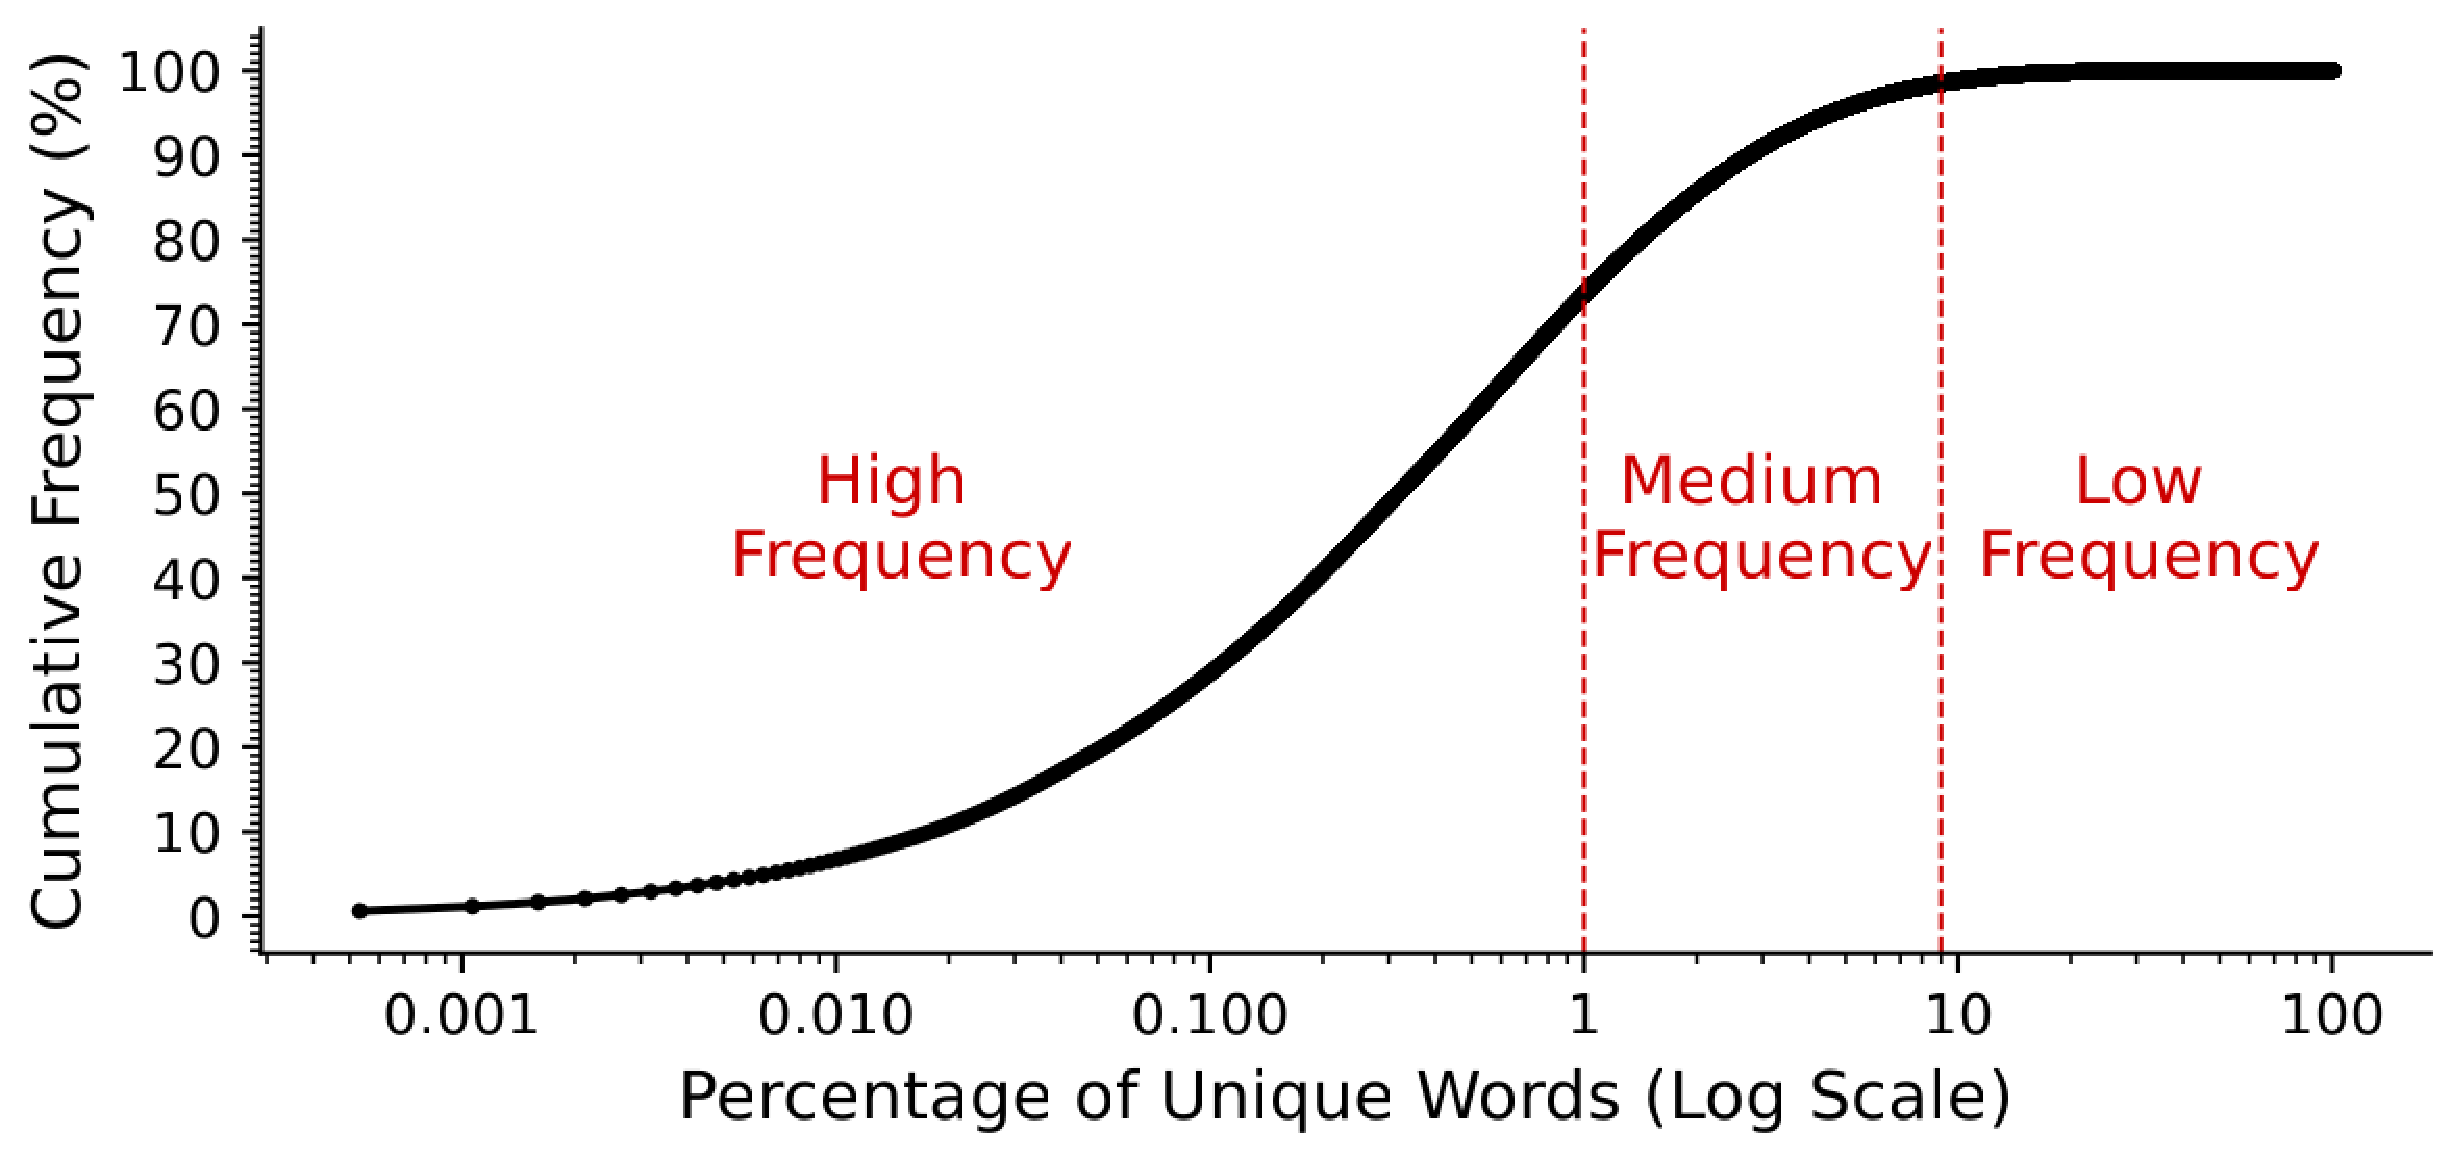
\includegraphics[width=0.5\linewidth]{flexheap/fig/method/words_freq.pdf}
	\caption{Distribution of words by their exact frequency in the dataset used for Lucene microbenchmarks.}
	\label{fig:words_freq}
\end{figure}

We use a \SI{300}{GB} real-world dataset~\cite{commoncr84:online} that contains 52.6 billion words.
To build our queries, we first perform a word count to determine the exact number of frequency for each word.
Then, we remove stop-words, single-character words, and non-English words.
Figure~\ref{fig:words_freq} shows the cumulative distribution of words (after selection) by their exact frequency.

Based on these counts, we classify the words into three categories: high-frequency, medium-frequency, and low-frequency.
The top 1\% of words are classified as high-frequency, accounting for 80\% of total occurrences.
In contrast, 91\% of words are low-frequency, representing only 1\% of total occurrences.
The remaining words fall into the medium-frequency category.
These frequency thresholds help us simulate different levels of I/O load during query processing.
High-frequency words appear in more documents within the Lucene index, resulting in higher I/O due to the need to access more documents.
In contrast, low-frequency words generate less I/O.
By using these frequency categories, we can effectively simulate varying I/O loads and analyze their impact on query performance.

We create small and large queries that fetch the top 50 or top \num{500000} results, respectively.
Unlike small queries, large queries require more memory in the managed heap because they create more memory pressure.
On the one hand, the frequency dimension (i.e., high, medium, and low) affects I/O.
Conversely, the number of results affects pressure in the managed heap.
Table~\ref{tab:lucene_queries} shows the performance implications of DRAM allocation between the managed heap and the I/O cache under different query loads.
Note that we omit running low-frequency queries with \num{500000} results since their results are typically fewer than 1000.

% \input{flexheap/tab_lucene_queries}
%
% \input{flexheap/tab_lucene_mixes}

\setlength\heavyrulewidth{1pt}
\begin{table}[h]
	\centering
	\begin{minipage}{0.55\textwidth}
		\centering
		\caption{Description of the mixes of Lucene queries.}
		\resizebox{\textwidth}{!}{%
			\begin{tabular}{l|ccc|cc}
				\textbf{\begin{tabular}[c]{@{}l@{}}\end{tabular}}                   & \multicolumn{3}{c|}{\textbf{Top 50}}                          & \multicolumn{2}{c}{\textbf{Top 500,000}}                                                                                                                                                                                                                             \\ \cline{2-6}
				\textbf{\begin{tabular}[c]{@{}l@{}}\end{tabular}}                   & \textbf{\begin{tabular}[c]{@{}c@{}}High\\ (H50)\end{tabular}} & \textbf{\begin{tabular}[c]{@{}c@{}}Medium\\ (M50)\end{tabular}} & \textbf{\begin{tabular}[c]{@{}c@{}}Low\\ (L50)\end{tabular}} & \textbf{\begin{tabular}[c]{@{}c@{}}High\\ (H500k)\end{tabular}} & \textbf{\begin{tabular}[c]{@{}c@{}}Medium\\ (M500k)\end{tabular}} \\ \cline{2-6}
				\textbf{Number of Queries}                                          & 40,000                                                        & 80,000                                                          & 240,000                                                      & 300                                                             & 6,000                                                             \\
				\textbf{\begin{tabular}[c]{@{}l@{}}GC overhead (\%)\end{tabular}}   & 0.1                                                           & 0.2                                                             & 0.7                                                          & 21                                                              & 30                                                                \\
				\textbf{\begin{tabular}[c]{@{}l@{}}I/O per query (MB)\end{tabular}} & 30                                                            & 10                                                              & 3                                                            & 31                                                              & 2                                                                 \\
				\bottomrule
			\end{tabular}
		}
		\label{tab:lucene_queries}
	\end{minipage}
	\hfill
	\begin{minipage}{0.42\textwidth}
		\centering
		\caption{Configuration of Lucene workloads.}
		\resizebox{\textwidth}{!}{%
			\begin{tabular}{lcl}
				                            & \textbf{Id} & \textbf{Queries description} \\ \hline
				\multirow{1}{*}{Sequential} & M1          & H50-M500k-L50-H500k-M50      \\ \hline
				\multirow{3}{*}{Concurrent} & M2          & H50-M500k-H500k              \\
				                            & M3          & M50-M500k-H500k              \\
				                            & M4          & L50-M500k-H500k              \\ \hline
			\end{tabular}
		}
		\label{tab:lucene_workloads}
	\end{minipage}
\end{table}

As shown in Table~\ref{tab:lucene_workloads}, we construct four experimental configurations using the query categories described in Table~\ref{tab:lucene_queries}.
%
M1 executes queries of different types sequentially without mixing them.
All queries in H50 (high frequency top 50 results) run before any of the M500k queries, etc.
Queries in each type are executed from 32 clients.
%
For the last three configurations (concurrent), we use 16 clients to execute the small queries, and another 16 clients execute the large queries concurrently.
The large queries arrive in batches based on a Poisson distribution, which aims to reflect the random nature of real-world query arrival rates.
This approach helps us understand how the system handles a diverse and concurrent query load, reflecting real-world usage more accurately.
To investigate future setups where the index size is significantly larger than the available DRAM, we use two different DRAM budgets: one where the DRAM budget equals 5\% and another where it equals 10\% of the index size as stored on the disk.
We allow OpenJDK ergonomics to set up the number of STW and concurrent GC threads.

\paragraph{\textbf{Baselines}}
We compare \flexheapName{} against two classes of dynamic heap resizing: G1 (GC-based) and VG1 (occupancy-based, time-driven).
To compare against the latest G1 heap resizing mechanism, we port its resizing policy from OpenJDK 26 to OpenJDK 21.
VG1 remains unchanged across JDK versions.
For Elasticsearch, we follow the official guidelines~\cite{elasticsearch:guidelines} and cap G1 at 50\% of DRAM (G1-50), leaving the remainder to the I/O cache.
We omit G1-90 from the main Elasticsearch evaluation because, as shown in Section~\S~\ref{flexheap:sec:motiv}, it consistently results in longer execution time than G1-50.
Accordingly, G1-50 serves as the strongest G1 baseline recommended for deployment.
For Spark, we cap the maximum heap at 75\% of DRAM (G1-75), following the guidelines of Spark 4.0.1~\cite{spark:guidelines}.
We configure VG1 to trigger a \flexheapGC{} every second to resize the heap and release memory back to the OS, as in prior work~\cite{bruno:resize}.
In Elasticsearch, VG1’s maximum heap is capped at 90\% of the DRAM budget, whereas in Spark it is capped at 75\%.
\flexheapName{} uses the same maximum heap cap as VG1 for each workload.
We note that in Spark, all systems use the same maximum heap cap, therefore, any differences are due to the heap resizing policy.

\section{Evaluation}
\label{flexheap:sec:eval}

\subsection{Performance Compared to GC-Based Resizing Mechanisms}
Figure~\ref{fig:es_g1_throughput} depicts ingestion and search throughput for Elasticsearch under G1-50 and \flexheapName{}, corresponding to the first and third bars in each group.
The results are normalized to G1-50 (higher is better).
\flexheapName{} improves ingestion throughput by 5--20\% over G1-50 by allowing more DRAM to flow to the heap during ingestion phases with high allocation pressure, which reduces GC frequency and avoids full GCs caused by the 50\% cap.
For example, in the Wikipedia workload with an \SI{8}{GB} DRAM budget, G1-50 incurs 17 full GCs during ingestion whereas \flexheapName{} incurs none.
\flexheapName{} also improves search throughput by up to $7\times$, driven by lower device I/O, with read traffic reduced by up to 30\% in the dense vector workload, as shown in Table~\ref{tab:es_traffic}.
For example, in the Wikipedia workload the average I/O wait falls from 23\% (G1-50) to 17\% with \flexheapName{}, allowing the I/O cache to serve more requests and sustain a higher query rate.

\begin{figure*}[t]
	
\includegraphics[width=0.25\linewidth]{flexheap/fig/eval/es_g1_fh_legend.pdf}
	\\
	\subfloat[Wikipedia]{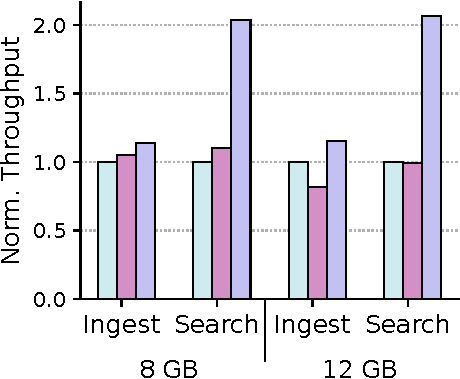
\includegraphics[width=0.245\linewidth]{flexheap/fig/eval/es_wiki.pdf}}
	\subfloat[Cohere Vector]{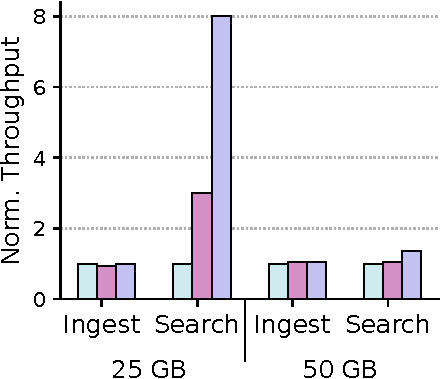
\includegraphics[width=0.245\linewidth]{flexheap/fig/eval/es_cv.pdf}}
	\subfloat[Dense Vector]{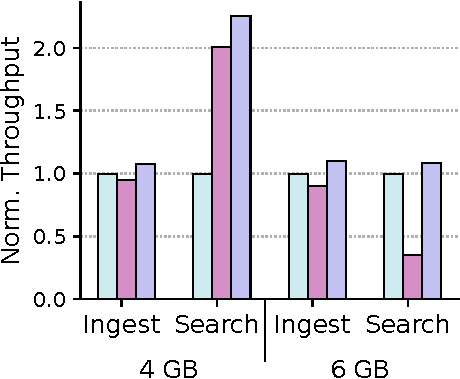
\includegraphics[width=0.245\linewidth]{flexheap/fig/eval/es_dv.pdf}}
	\subfloat[OpenAI Vector]{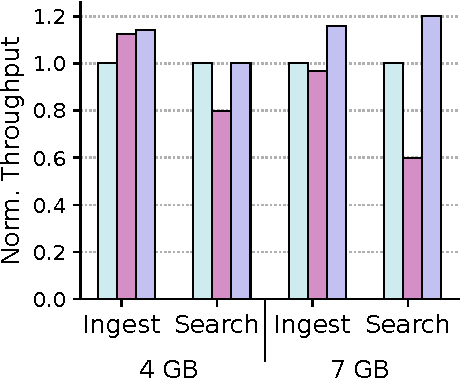
\includegraphics[width=0.245\linewidth]{flexheap/fig/eval/es_ai.pdf}}
	\caption{Ingestion and search throughput for Elasticsearch workloads under
		G1-50 (maximum heap cap of 50\% of DRAM), VG1, and \flexheapName{}.}
	\label{fig:es_g1_throughput}
\end{figure*}

% \begin{table}[t]
% 	\caption{Read and write I/O traffic for Elasticsearch workloads under G1-50
% 		and \flexheapName{} (FH) in small DRAM budget configurations.}
% 	\label{tab:es_traffic}
% 	\resizebox{0.5\columnwidth}{!}{%
% 		\begin{tabular}{llll|lll}
% 			              & \multicolumn{3}{c|}{\textbf{Read Traffic}} & \multicolumn{3}{c}{\textbf{Write Traffic}}                                                                                                                                                   \\
% 			              & \multicolumn{1}{c}{\textbf{G1-50}}         & \multicolumn{1}{c}{\textbf{FH}}            & \multicolumn{1}{c|}{\textbf{Diff}} & \multicolumn{1}{c}{\textbf{G1-50}} & \multicolumn{1}{c}{\textbf{FH}}   & \multicolumn{1}{c}{\textbf{Diff}} \\
% 			              & \multicolumn{1}{c}{\textbf{(GB)}}          & \multicolumn{1}{c}{\textbf{(GB)}}          & \multicolumn{1}{c|}{\textbf{(\%)}} & \multicolumn{1}{c}{\textbf{(GB)}}  & \multicolumn{1}{c}{\textbf{(GB)}} & \multicolumn{1}{c}{\textbf{(\%)}} \\ \hline
% 			Wikipedia     & 1677                                       & 1444                                       & \textbf{-14\%}                     & 637                                & 605                               & \textbf{-5\%}                     \\
% 			Cohere Vector & 29862                                      & 23636                                      & \textbf{-21\%}                     & 331                                & 334                               & +0.9\%                            \\
% 			Dense Vector  & 189                                        & 134                                        & \textbf{-29\%}                     & 79                                 & 85                                & +7\%                              \\
% 			OpenAi        & 716                                        & 638                                        & \textbf{-10\%}                     & 467                                & 432                               & \textbf{-7\%}                     \\ \hline
% 		\end{tabular}
% 	}
% \end{table}

\begin{table}[t]
	\caption{Read and write I/O traffic for Elasticsearch workloads under G1-50 (maximum heap cap
		of 50\% of DRAM), VG1, and \flexheapName{} (FH) in small DRAM budget configurations.}
	\label{tab:es_traffic}
	\resizebox{\columnwidth}{!}{%
		\begin{tabular}{l|ccccc|ccccc}
			\toprule
			              & \multicolumn{5}{c|}{\textbf{Read Traffic}} & \multicolumn{5}{c}{\textbf{Write Traffic}}                                                                                                                                                          \\
			\cmidrule(lr){2-6} \cmidrule(lr){7-11}
			              & \textbf{G1-50}                             & \textbf{VG1}                               & \textbf{FH}   & \textbf{Diff}        & \textbf{Diff}      & \textbf{G1-50} & \textbf{VG1}  & \textbf{FH}   & \textbf{Diff}        & \textbf{Diff}      \\
			              & \textbf{(GB)}                              & \textbf{(GB)}                              & \textbf{(GB)} & \textbf{FH vs G1-50} & \textbf{FH vs VG1} & \textbf{(GB)}  & \textbf{(GB)} & \textbf{(GB)} & \textbf{FH vs G1-50} & \textbf{FH vs VG1} \\
			\midrule
			Wikipedia     & 1677                                       & 3442                                       & 1444          & \textbf{-14\%}       & \textbf{-57\%}     & 637            & 587           & 605           & \textbf{-5\%}        & +3\%               \\
			Cohere Vector & 29862                                      & 27100                                      & 23636         & \textbf{-21\%}       & \textbf{-13\%}     & 331            & 336           & 334           & +0.9\%               & \textbf{-0.6\%}    \\
			Dense Vector  & 189                                        & 468                                        & 134           & \textbf{-29\%}       & \textbf{-71\%}     & 79             & 79            & 85            & +7\%                 & +7\%               \\
			OpenAI        & 716                                        & 700                                        & 638           & \textbf{-10\%}       & \textbf{-8\%}      & 467            & 435           & 432           & \textbf{-7\%}        & \textbf{-0.7\%}    \\
			\bottomrule
		\end{tabular}
	}
\end{table}


Next, we evaluate \flexheapName{} against G1 in Spark.
Figures~\ref{fig:spark_g1}(a) and \ref{fig:spark_g1}(b) report per-query speedups on TPC-DS with \SI{16}{\giga\byte} and \SI{32}{\giga\byte} DRAM budgets.
\flexheapName{} delivers more than 10\% speedups on roughly 40\% of queries with a \SI{16}{\giga\byte} DRAM budget and on 27\% of queries with \SI{32}{\giga\byte}.
The gains are smaller at \SI{32}{\giga\byte} because the larger DRAM budget leaves a larger I/O cache even under G1, reducing the headroom for \flexheapName{} to improve I/O performance.
The gains correlate with lower device pressure: read I/O drops by up to 30\%, because \flexheapName{} reassigns DRAM from the heap to the I/O cache during I/O-intensive phases and grows the heap when allocation pressure rises.
As a concrete example highlighted in Figures~\ref{fig:spark_g1}(c) and (d), q28 improves by 50\% when \flexheapName{} maintains a smaller committed heap throughout the run, which preserves a larger I/O cache and cuts average I/O wait by about 30\%.
For queries where \flexheapName{} matches G1, the traces show little or no I/O bottleneck, so I/O cache size is not the limiting factor and both mechanisms exhibit similar I/O traffic.

\begin{figure*}[h]
	
\includegraphics[width=0.6\linewidth]{flexheap/fig/eval/spark/analysis/legend.pdf}
	\\
	\subfloat[16\:GB]{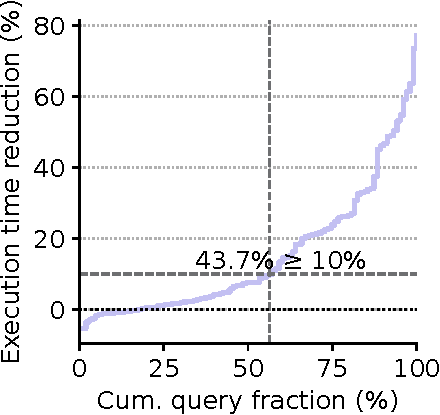
\includegraphics[width=0.24\linewidth]{flexheap/fig/eval/spark/tpcds_g1_fh.pdf}}
	\subfloat[32\:GB]{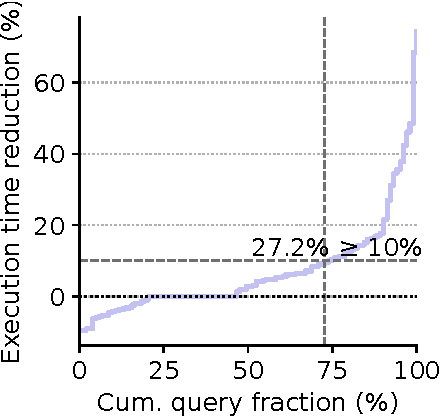
\includegraphics[width=0.24\linewidth]{flexheap/fig/eval/spark/tpcds_g1_fh_32g.pdf}}
	\subfloat[Q28-G1]{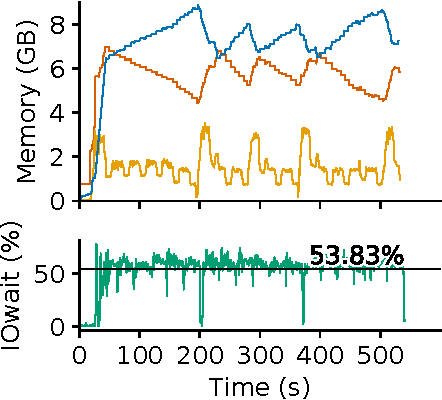
\includegraphics[width=0.24\linewidth]{flexheap/fig/eval/spark/analysis/q28_g1_10g_16g.pdf}}
	\subfloat[Q28-FlexHeap]{\includegraphics[width=0.24\linewidth]{flexheap/fig/eval/spark/analysis/q28_fh_10g_16g.pdf}}
	\caption{Performance improvement of \flexheapName{} over G1-75 (maximum heap cap 75\% of
		DRAM) heap resizing in Spark-SQL on TPC-DS.}
	\label{fig:spark_g1}
\end{figure*}

% \begin{figure*}[h]
% 	
\includegraphics[width=0.5\linewidth]{flexheap/fig/eval/spark/analysis/legend.pdf}
% 	\\
% 	\subfloat[Q28-G1]{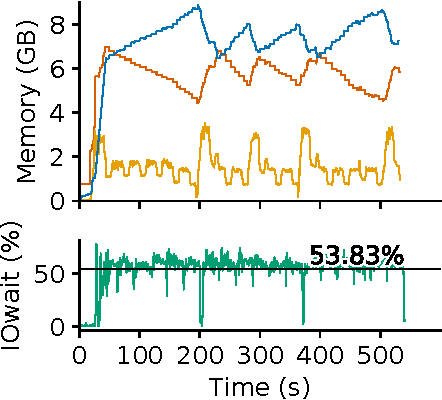
\includegraphics[width=0.24\linewidth]{flexheap/fig/eval/spark/analysis/q28_g1_10g_16g.pdf}}
% 	\subfloat[Q28-FH]{\includegraphics[width=0.24\linewidth]{flexheap/fig/eval/spark/analysis//q28_fh_10g_16g.pdf}}
% 	\subfloat[Q66-G1]{\includegraphics[width=0.24\linewidth]{flexheap/fig/eval/spark/analysis/q66_g1_10g_16g.pdf}}
% 	\subfloat[Q66-FH]{\includegraphics[width=0.24\linewidth]{flexheap/fig/eval/spark/analysis/q66_fh_10g_16g.pdf}}
% 	\caption{q28}
% 	\label{fig:q28}
% \end{figure*}

\subsection{Performance Compared to Occupancy-Based Resizing Mechanisms}

We investigate the performance of \flexheapName{} compared to VG1 in Elasticsearch.
As shown in Figure~\ref{fig:es_g1_throughput} (second and third bars in each group), across all four workloads, ingestion throughput under \flexheapName{} is higher than or comparable to VG1.
For Wikipedia and OpenAI Vector, ingestion throughput is similar between the two policies.
For Dense Vector and Cohere Vector, \flexheapName{} outperforms VG1 in ingestion by up to 30\%.
These workloads perform updates to the index during ingestion, which include not only writes but also reads of existing segments; these updates benefit from a larger I/O cache.
For search operations, \flexheapName{} delivers substantially higher throughput compared to VG1, by up to $2\times$ in Wikipedia, and by up to $5\times$ in Cohere Vector.
During the period when search runs alongside ingestion, \flexheapName{} shrinks the heap in response to I/O pressure and reserves more DRAM for the I/O cache, raising cache hit rates and reducing I/O wait for queries.
For example, as shown in Table~\ref{tab:es_traffic}, the read traffic to the device improves up to 71\% compared to \flexheapName{}.
VG1 keeps the heap near its maximum heap size in this phase (as shown in our motivation), which starves the I/O cache and limits search throughput despite similar ingestion rates.

Next, we show how \flexheapName{} affects the performance of TPC-DS queries in Spark over VG1 (Figures~\ref{fig:spark_vg1}(a, b)).
Using \flexheapName{}, about 30\% and 26\% of queries have execution time reduction compared to VG1 for \SI{16}{GB} and \SI{32}{GB} DRAM budgets, respectively.
Most of the improvements come from reducing I/O wait time.
To explain this pattern, we show what happens during execution of q28 (Figures~\ref{fig:spark_vg1}(c, d)).
Under VG1, illustrated in Figure~\ref{fig:spark_vg1}(c), the heap committed memory increases and stays high, the I/O cache is small with a sawtooth pattern, and I/O-wait stays elevated across the run.
Under FlexHeap, depicted in Figure~\ref{fig:spark_vg1}(d), the heap is kept lower and adjusted more often, the I/O cache is larger across the run, and I/O-wait collapses to short bursts.
These decisions reduce average I/O wait time from 54\% to 27\%, reducing the query’s wall time by roughly $2\times$.

% \begin{figure*}[t]
% 	\includegraphics[width=0.2\linewidth]{flexheap/fig/eval/vg1/es_vg1_fh_legend.pdf}
% 	\\
% 	\subfloat[Wikipedia]{\includegraphics[width=0.245\linewidth]{flexheap/fig/eval/vg1/es_wiki.pdf}}
% 	\subfloat[Cohere Vector]{\includegraphics[width=0.245\linewidth]{flexheap/fig/eval/vg1/es_cv.pdf}}
% 	\subfloat[Dense Vector]{\includegraphics[width=0.245\linewidth]{flexheap/fig/eval/vg1/es_dv.pdf}}
% 	\subfloat[Openai Vector]{\includegraphics[width=0.245\linewidth]{flexheap/fig/eval/vg1/es_ai.pdf}}
% 	\caption{Ingestion and search throughput for Elasticsearch workloads under
% 		VG1 and FlexHeap.}
% 	\label{fig:es_vg1}
% \end{figure*}

% \input{flexheap/tab_es_vg1_traffic}

\begin{figure*}[t]
	
\includegraphics[width=0.6\linewidth]{flexheap/fig/eval/spark/analysis/legend.pdf}
	\\
	\subfloat[16 GB]{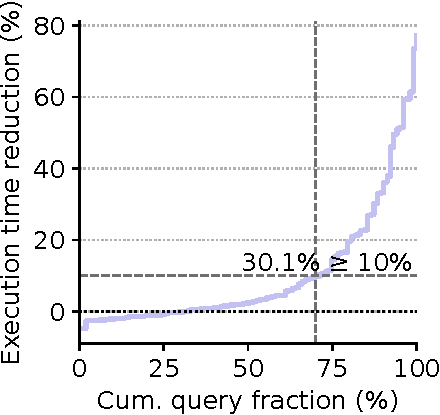
\includegraphics[width=0.245\linewidth]{flexheap/fig/eval/spark/tpcds_vg1_fh.pdf}}
	\subfloat[32 GB]{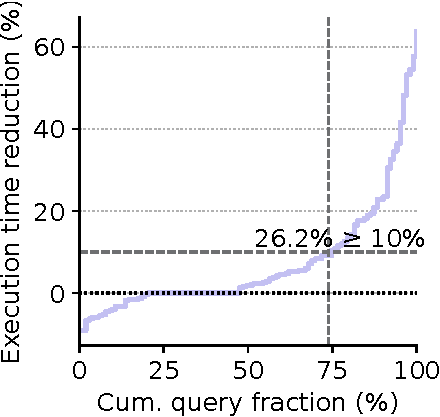
\includegraphics[width=0.245\linewidth]{flexheap/fig/eval/spark/tpcds_vg1_fh_32g.pdf}}
	\subfloat[Q28-VG1]{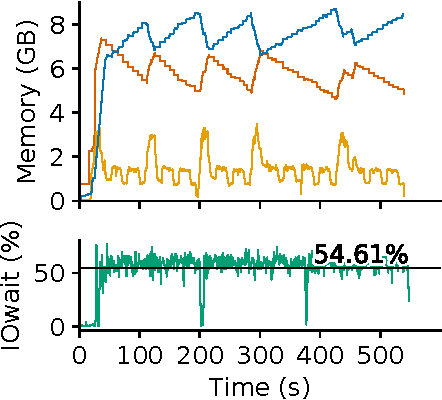
\includegraphics[width=0.245\linewidth]{flexheap/fig/eval/spark/analysis/q28_je_10g_16g.pdf}}
	\subfloat[Q28-FlexHeap]{\includegraphics[width=0.245\linewidth]{flexheap/fig/eval/spark/analysis/q28_fh_10g_16g.pdf}}
	\caption{Performance improvement of \flexheapName{} compared to VG1 in Spark-SQL on TPC-DS.}
	\label{fig:spark_vg1}
\end{figure*}


\subsection{Effects on Tail-Latency for Elasticsearch}

We investigate how the decisions of \flexheapName{} affect the p99 tail-latency of Elasticsearch queries compared to G1 and VG1.
Figure~\ref{fig:es_latency}(a, b) shows the p99 latency of ingestion and search tasks for all the workloads, respectively.

For ingestion tasks, with larger DRAM budgets, \flexheapName{} lowers p99 latency compared to G1-50 because it can grow the heap (up to 90\% of DRAM) when allocation pressure spikes, avoiding queueing and cap-induced full GCs.
On Cohere-Vector, \flexheapName{} reduces p99 by about 10\% compared to G1-50 and by up to 30\% compared to VG1.
VG1’s periodic reclamation rarely triggers during ingestion (the heap is actively used) so its latency typically sits near or slightly above G1’s.
With smaller budgets, \flexheapName{} still reduces p99 by 5--10\% compared to G1, chiefly by cutting GC pressure (in our traces, young/mixed GC counts often drop by about $2\times$) and eliminating cap-driven full GCs.
Moreover, because VG1 keeps the heap near its maximum heap size and leaves less DRAM for the I/O cache, Elasticsearch’s segment flushes during ingestion run against a smaller write-back buffer and take longer.
By preserving more I/O cache, \flexheapName{} reduces flushes and further reducing tail latency.

For search tasks, \flexheapName{} lowers p99 across all DRAM budgets because it reacts to I/O stalls by shrinking the heap and enlarging the I/O cache, which increases cache residency, reduces device read traffic, and shortens queueing at the storage layer.
The effect is strongest with small budgets: on Wikipedia at \SI{8}{GB}, VG1’s p99 is about $1.6\times$ higher than G1 because it keeps the heap near the cap and starves the cache, while \flexheapName{} is about 25\% below G1.
At \SI{12}{GB}, \flexheapName{} remains lower than both mechanisms.
On OpenAI Vector, VG1 sometimes improves latency relative to G1 because it returns memory to the OS more often after the ingestion phase.
\flexheapName{} improves performance further because its shrink decisions consider I/O stalls rather than occupancy targets, resulting in bigger steps of memory release.

\begin{figure*}[h]
	
\includegraphics[width=0.25\linewidth]{flexheap/fig/eval/es_g1_fh_legend.pdf}
	\\
	\subfloat[Ingestion]{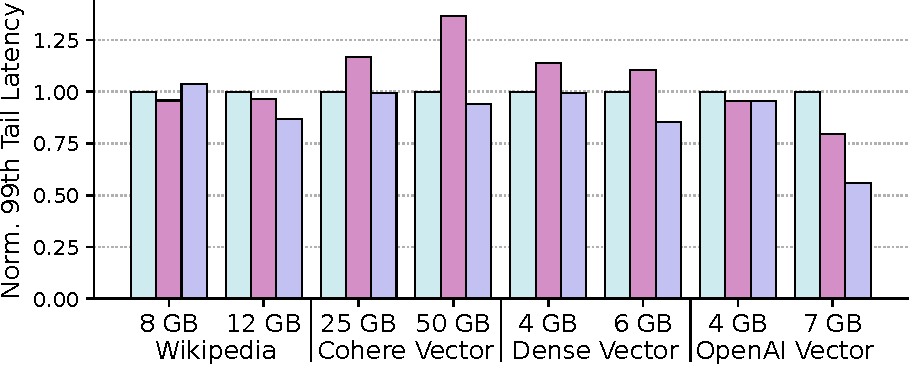
\includegraphics[width=0.495\linewidth]{flexheap/fig/eval/es_ingest_lat.pdf}}
	\subfloat[Search]{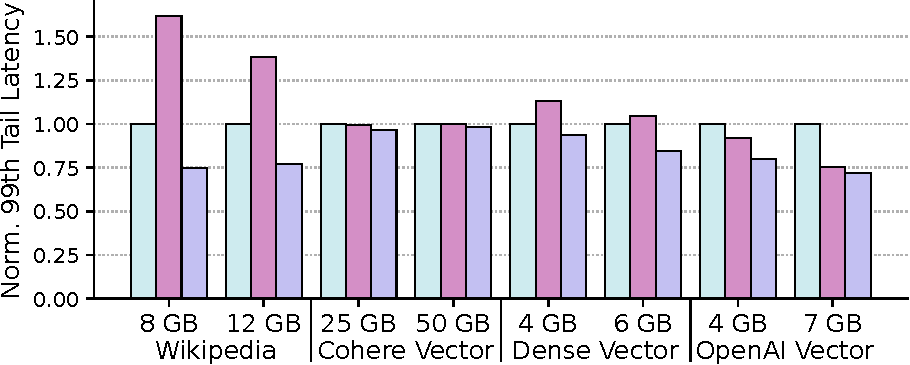
\includegraphics[width=0.495\linewidth]{flexheap/fig/eval/es_search_lat.pdf}}
	\caption{P99 latency of (a) ingestion and (b) search tasks for Elasticsearch
		with G1-50 (maximum heap cap 50\% of DRAM), VG1, and \flexheapName{}.}
	\label{fig:es_latency}
\end{figure*}

\subsection{Sensitivity Analysis}

\paragraph{\textbf{Sensitivity to application phase changes.}}
Here, we investigate how \flexheapName{} adapts to application phases using M1 workload of Lucene.
Compared to G1 (Figure~\ref{fig:phases}(a)), FlexHeap (Figure~\ref{fig:phases}(b)) tracks the application’s five phases much more closely by continuously rebalancing heap and I/O cache memory.
Under G1, the heap quickly grows near its maximum and stays there, pushing the I/O cache down and keeping it low, whereas FlexHeap shrinks and regrows the heap at each phase boundary, leaving several additional gigabytes available in the I/O cache for I/O.
This adaptation shortens multiple phases: the first phase finishes in about 350 s with FlexHeap versus 400 s with G1, and the second phase is dramatically shorter (150 s versus 350 s).
The long final phase is also reduced from roughly 600 s with G1 to about 200 s with FlexHeap.
By maintaining a significantly larger I/O cache and reacting quickly to phase changes, FlexHeap reduces I/O stalls and GC overhead, which directly translates into a substantially lower execution time by 40\%.

\begin{figure*}[h]
	
\includegraphics[width=0.5\linewidth]{flexheap/fig/eval/micro/legend.pdf}
	\\
	\subfloat[G1-90]{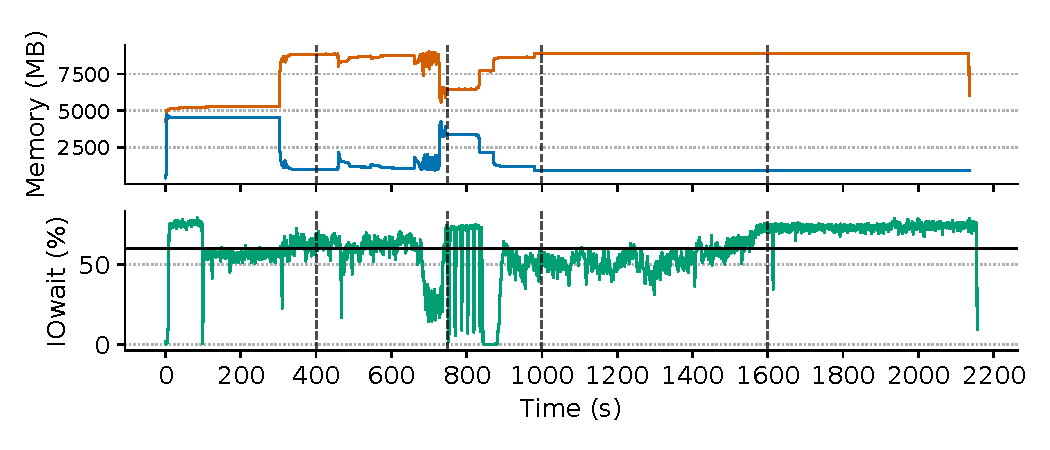
\includegraphics[width=0.495\linewidth]{flexheap/fig/eval/micro/g1_m1.pdf}}
	\subfloat[FlexHeap]{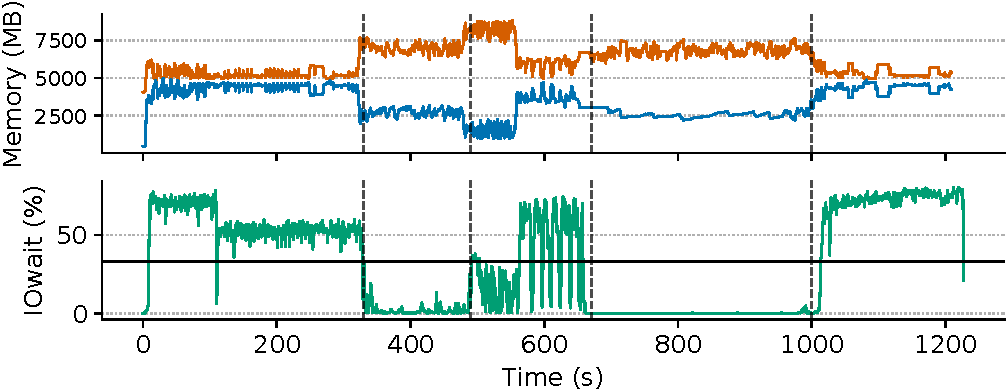
\includegraphics[width=0.495\linewidth]{flexheap/fig/eval/micro/fh_m1.pdf}}
	\caption{Execution of M1 workload over time using (a) G1-90 and (b) \flexheapName{}
		with maximum heap cap 90\% of DRAM budget.}
	\label{fig:phases}
\end{figure*}

\paragraph{\textbf{Sensitivity to device latency.}}
We investigate the benefits of using \flexheapName{} when Lucene utilizes SATA SSDs, which have higher latency than NVMe SSDs but are more cost-effective for storing Lucene's index.
SATA SSDs differ from NVMe SSDs in terms of interface and speed.
NVMe SSDs use the PCIe interface, which provides faster data transfer speed than SATA SSDs that use the older SATA interface.
Also, the read and write throughput of our NVMe SSD is 6$\times$ and 4$\times$ higher compared to SATA SSD, respectively.

\begin{figure}[h]
	\centering
	
\includegraphics[width=0.2\linewidth]{flexheap/fig/eval/sensitivity/lucene_sata_nvme_legend-crop.pdf}
	\hspace{10pt}
	
\includegraphics[width=0.25\linewidth]{flexheap/fig/eval/sensitivity/lucene_breakdowns_legend-crop.pdf}
	\\
	\subfloat[Throughput]{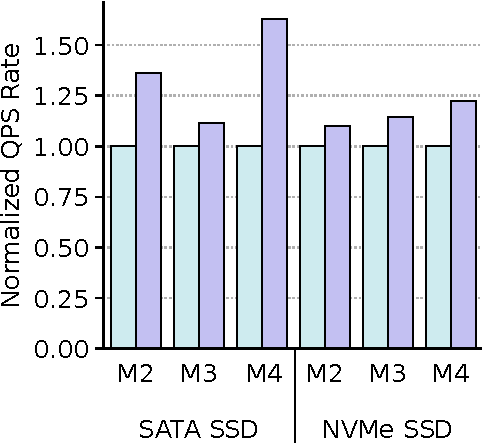
\includegraphics[width=0.25\linewidth]{flexheap/fig/eval/sensitivity/lucene_sata_nvme_qps-crop.pdf}}
	\hspace{10pt}
	\subfloat[GC and IO wait time]{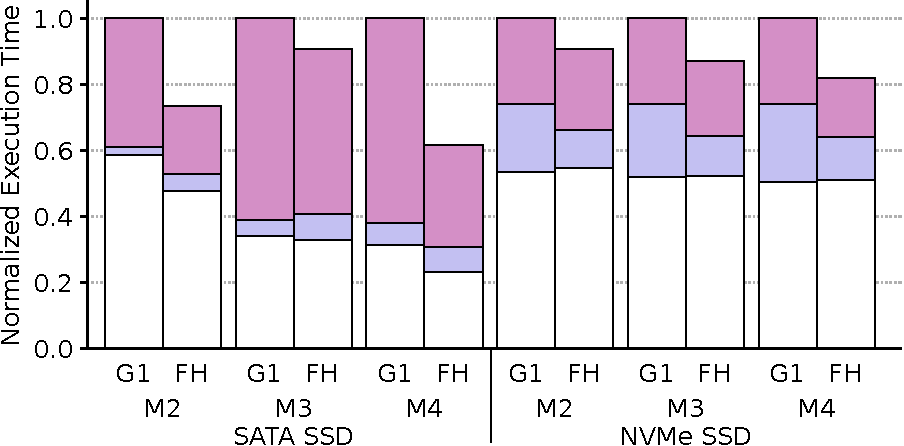
\includegraphics[width=0.45\linewidth]{flexheap/fig/eval/sensitivity/lucene_sata_nvme_breakdowns-crop.pdf}}
	\caption{Lucene (a) throughput and (b) execution time breakdown, comparing G1 and \flexheapName{} (FH) on SATA SSD and NVMe SSD using \SI{5}{GB} DRAM budget.}
	\label{flexheap:fig:sata_ssd}
\end{figure}

Figures~\ref{flexheap:fig:sata_ssd}(a, b) illustrate the throughput and the \flexheapGC{} and I/O wait times for Lucene using SATA SSD and NVMe SSD with a \SI{5}{GB} DRAM budget, respectively.
\flexheapName{} consistently outperforms G1 across all workloads for both types of SSDs.
Notably, the throughput improvement is more pronounced with SATA SSDs, where \flexheapName{} increases throughput by up to 60\% compared to G1, highlighting its effectiveness in environments with higher latency storage.
As shown in Figure~\ref{flexheap:fig:sata_ssd}(b), in experiments with SATA SSD, \flexheapName{} increases \flexheapGC{} time by up to 2.1$\times$ compared to G1 because it prioritizes reducing I/O overhead due to the higher latency of the device.
However, with the reduces latency of NVMe SSDs, the \flexheapGC{} overhead becomes a more significant bottleneck compared to I/O.
Consequently, \flexheapName{} shifts focus to targeting \flexheapGC{} overhead, reducing \flexheapGC{} time by up to 46\% compared to G1.
By dynamically targeting both I/O and \flexheapGC{} overheads, \flexheapName{} adapts effectively to the changing device latency, increasing performance.

\paragraph{\textbf{Sensitivity to resizing step.}}
We evaluate \flexheapName{}’s sensitivity to reallocation step sizes using the M1 workload of Lucene with \SI{5}{GB}, \SI{10}{GB}, \SI{18}{GB}, and \SI{27}{GB} of DRAM (Figure~\ref{fig:reallocation_step}).
The optimal static step varies across DRAM budgets, making offline configuration challenging.
In contrast, the adaptive approach consistently outperforms the best static steps in most cases, with only a 5\% slowdown in the \SI{10}{GB} configuration.
A static 80\% step results in up to $7.7\times$ higher \flexheapGC{} time, highlighting the efficiency of adaptive reallocation.

\begin{figure}[h]
	\centering
	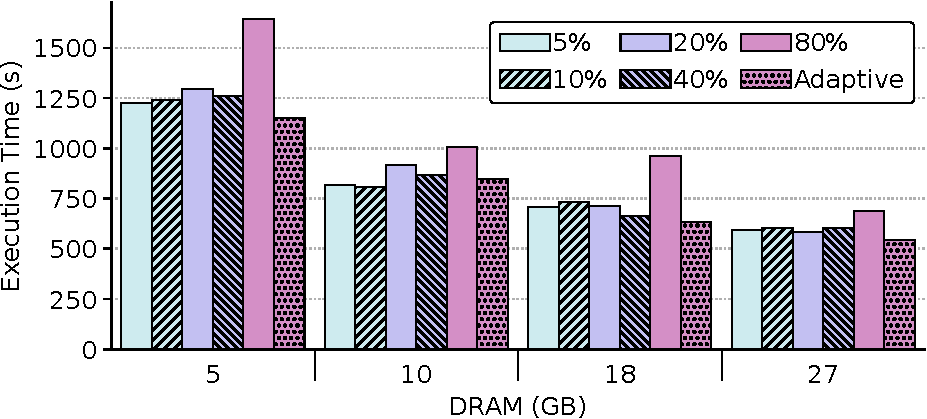
\includegraphics[width=0.5\linewidth]{flexheap/fig/eval/sensitivity/resizing_step-crop.pdf}
	\caption{Execution time of M1 workload in Lucene using static and adaptive reallocation steps for different DRAM budgets.}
	\label{fig:reallocation_step}
\end{figure}

\section{Conclusions}

Popular search engines and analytic frameworks running on JVM must carefully balance memory between the JVM heap and the I/O cache to achieve high performance.
Existing heap resizing mechanisms focus solely on reducing GC overhead, neglecting the cost of I/O stalls.
%
In this paper, we propose \flexheapName{}, a heap resizing mechanism for G1 that dynamically partitions memory between the heap and the I/O cache.
Between GC intervals, \flexheapName{} estimates the CPU time lost to GC and to I/O stalls, and repartitions DRAM to reduce their combined cost.
It makes frequent decisions at G1 collection boundaries, relies on a history-based model to project future GC and I/O stall costs, and adapts its resizing step proportional to the magnitude of changes in that combined cost.
%
Our evaluation shows that \flexheapName{} improves throughput in Elasticsearch and Spark by an average 30\% and 33\%, respectively.
Also, \flexheapName{} outperforms VG1 by on average 50\%.
These results demonstrate that I/O-aware heap resizing is important for improving performance in modern JVM-based search and analytic applications.

\section{Data Availability Statement}
The artifact containing the code and the benchmarks of this paper is available at \url{https://github.com/CARV-ICS-FORTH/flexheap} or alternatively a static version is available at \url{https://doi.org/10.5281/zenodo.19183591}.

\section*{Chapter Summary}
Popular JVM-based search and analytics systems, such as Elasticsearch and Spark, rely on the OS page cache (I/O cache) to accelerate storage access.
However, dividing memory between the JVM heap and the I/O cache creates a trade-off: enlarging the heap reduces garbage collection (GC) overhead but starves the I/O cache, while shrinking it improves I/O performance but raises GC cost.
Existing heap resizing mechanisms ignore I/O and thus fail to address this trade-off, resulting in inefficient memory utilization and degraded performance.

In this paper, we propose \flexheapName{}, a heap resizing mechanism for Garbage First (G1), the default OpenJDK garbage collector, that dynamically partitions a fixed DRAM budget between the JVM heap and the I/O cache.
Between GC intervals, it estimates the CPU time lost to GC and to I/O stalls and repartitions DRAM to reduce their combined cost.
\flexheapName{} relies on three concepts:
	%
(1) It makes resizing decisions using G1 collection boundaries.
	%
(2) It uses a history-based approach to estimate the cost of \flexheapGC{} and I/O stalls for the future intervals.
	%
(3) It uses an adaptive resizing step that scales with changes in the combined cost.

We implement \flexheapName{} in OpenJDK 21’s G1 garbage collector and evaluate it on two widely used systems: the Elasticsearch search engine and the Spark analytic framework.
Compared to the G1 heap resizing mechanism, \flexheapName{} improves performance by an average of 30\% in Elasticsearch and by an average of 33\% in Spark.
It outperforms Vertical G1, a state-of-the-art enhancement to the default G1 heap resizing mechanism, that returns unused memory to the OS eagerly, by 50\% on average in throughput, demonstrating that JVM heap resizing needs to consider I/O overhead in search and analytics applications.


\setstretch{1.15}

\chapter{Related Work}
\label{chapter:related}

This chapter reviews work related to the dissertation's three contributions: storage-backed managed heaps, garbage-collection and data-placement techniques, and dynamic coordination of JVM heap capacity with the operating-system page cache.
The first two contributions extend managed-object capacity onto storage while addressing collector costs under different collection goals.
The third contribution studies how the JVM heap and file cache should share DRAM, and can complement storage-backed heaps without itself implementing one.

\section{Extending Managed Heaps Beyond DRAM}

Several systems increase the memory available to managed applications by using secondary storage, non-volatile memory (NVM), or remote memory.
Their designs differ in whether objects retain their managed representation, how the collector discovers and reclaims them, and whether the target is local block-addressable storage or another memory tier.

\subsection{Local Storage-Backed Heaps}

LOOM extends object memory across DRAM and secondary storage~\cite{kaehler:loom}.
Other systems, including Abdelrahman and Pande's design, Melt, and LeakSurvivor, move cold or stale reachable objects to disk and restore them when accessed~\cite{abdelrahman:memorygc,bond:melt,leaksurvivor}.
These designs target objects with infrequent accesses and use mechanisms that differ from a memory-mapped managed heap.
Melt and LeakSurvivor maintain object-location metadata in the JVM, while LeakSurvivor also defers reclamation on disk until space is needed.
TMO monitors DRAM pressure and moves cold pages to slower tiers, including NVMe SSDs, below the JVM's object model~\cite{weiner:tmo}.

TeraHeap and Chipper instead expose a storage-backed heap in which objects retain their Java representations and are accessed through memory mapping.
TeraHeap integrates this heap with the throughput-oriented Parallel Scavenge collector and avoids scanning storage-resident objects during ordinary collection~\cite{teraheap,kolokasis:teracache}.
Chipper addresses a different constraint: it integrates storage migration with G1's incremental, pause-bounded collection policy, accounting for migration work when selecting regions for evacuation.
These designs share the goal of reducing serialization and storage-resident GC work, but their collector mechanisms and latency objectives differ.

Table~\ref{tab:related} summarizes selected systems that extend managed heaps beyond local DRAM according to developer effort, whether GC scans the secondary tier, and device type.
The table reflects the taxonomy used to compare TeraHeap with prior heap-scaling systems; it is not a complete comparison of low-pause collector designs.

\setlength{\unitlength}{1em}

\begin{table}[t]
\centering
\caption{Comparison of selected systems that extend managed heaps beyond DRAM.}
\resizebox{0.8\columnwidth}{!}{%
\begin{tabular}{lccccc}
\hline
\multicolumn{1}{c}{\multirow{2}{*}{\textbf{System}}} &
  \multirow{2}{*}{\textbf{\begin{tabular}[c]{@{}c@{}}Developer \\ Effort\end{tabular}}} &
  \multicolumn{2}{c}{\textbf{\begin{tabular}[c]{@{}c@{}}GC Scans\\ on the Device\end{tabular}}} &
  \multicolumn{2}{c}{\textbf{Device Type}} \\ \cline{3-6}
\multicolumn{1}{c}{}         &      & \textbf{Lazy} & \textbf{Eager}       & \textbf{Block-addressable} & \textbf{Byte-addressable} \\ \hline
  LeakSurvivor~\cite{leaksurvivor}                  & High & (\checkmark)  & -                    & \checkmark                 & -                         \\
  Melt~\cite{bond:melt}                             & None & (\checkmark)  & -                    & \checkmark                 & -                         \\
  Write Rationing~\cite{akram:ration}               & None & -             & \checkmark           & -                          & \checkmark                \\
  Panthera~\cite{wang:Panthera}                     & Low  & -             & \checkmark           & -                          & \checkmark                \\
  NVM-friendly-GC~\cite{nvm-gc-eurosys}             & None & -             & \checkmark           & -                          & \checkmark                \\
  JPD Heap~\cite{jpd_heap}                     & High & -             & \checkmark           & -                          & \checkmark                \\
  GCMove~\cite{gcmove}                      & None & -             & \checkmark           & -                          & \checkmark                \\
  ThinGC~\cite{thingc}                      & None & -             & \checkmark           & -                          & \checkmark                \\
  TMO~\cite{weiner:tmo}                          & None & -             & \checkmark           & \checkmark                 & -                         \\
  Semeru~\cite{wang:semeru}                       & None & -             & \checkmark           & -                          & \checkmark                \\
  MemLiner~\cite{wang:memliner}                     & None & -             & \checkmark           & -                          & \checkmark                \\
  Mako~\cite{ma:mako}                         & None & -             & \checkmark           & -                          & \checkmark                \\ \hline
\textbf{TeraHeap (this thesis)} & Low  & \checkmark    & -                    & \checkmark                 & \checkmark                \\ \hline
\end{tabular}%
}
\label{tab:related}
\end{table}


\subsection{Byte-Addressable NVM and Remote Memory}

Work on byte-addressable NVM includes systems that place objects according to access or write hotness to reduce writes or improve performance~\cite{akram:ration,akram:crystal,gcmove,thingc}.
NVM-friendly-GC optimizes G1 for an NVM-resident heap and uses DRAM as a cache for collector operations~\cite{Xu:gc_evaluation}.
Panthera and JPDHeap place managed objects across DRAM and NVM, but allow the collector to scan NVM-resident objects~\cite{wang:Panthera,jpd_heap}.
These systems target byte-addressable media, whose access granularity and capacity differ from local NVMe SSDs.

Remote-memory systems address the cost of tracing and collecting objects across a network.
MemLiner improves far-memory locality by aligning collector access order with mutator access patterns~\cite{wang:memliner}.
Semeru separates execution and memory responsibilities across JVM instances, while Mako offloads object scanning and evacuation to memory servers~\cite{wang:semeru,ma:mako}.
DGC offloads concurrent marking to a remote garbage-collection service over RDMA~\cite{hongtao:dgc}.
SmartSweep explores reclamation of remote or tiered managed heaps by returning garbage-rich regions to local memory for collection~\cite{kolokasis:smartsweep}.
SmartSweep is an exploratory direction in this dissertation rather than a fourth principal contribution.

\section{Reducing Managed-Memory and Data-Movement Costs}

\subsection{Reducing Garbage-Collection Cost}

Some systems reduce GC cost while keeping application data in DRAM.
Facade and Gerenuk transform application code to use off-heap representations, reducing the amount of object data traced by the JVM~\cite{nguyen:facade,navasca:gerenuk}.
Broom groups objects with similar lifetimes into regions, while DSA uses programmer annotations to allocate selected data structures separately and improve tracing locality and parallelism~\cite{gog:broom,cohen:dsa}.
Yak allocates objects by programmer-defined epochs, and Deca uses lifetime information to manage Spark objects~\cite{khanh:yak,lu:deca}.
BridgeGC uses framework annotations to avoid repeatedly tracing and copying long-lived data until the framework signals its release~\cite{wang:bridgegc}.
NG2C and allocation-site profiling identify long-lived objects for pretenuring~\cite{bruno:n2gc,pretenuring,Blackburn:2001:PJ}.
These approaches reduce tracing, copying, or allocation overhead, but do not provide the capacity of a storage-backed heap.

\subsection{Reducing Serialization and Data-Movement Cost}

Serialization libraries such as Thrift, Kryo, and Protocol Buffers provide general-purpose formats and implementations for converting object graphs to and from byte streams~\cite{thrift,kryo,protocol-buffers}.
Other systems reduce conversion or transfer costs by moving managed object graphs directly between JVMs, as in Skyway, or by bypassing conventional serialization for RDMA or inter-JVM transfers, as in Naos and ZCOT~\cite{nguyen:skyway,taranov:naos,wu:zero_change}.
SSDStreamer uses a lightweight serializer and a stream-oriented I/O path for SSD-backed caching~\cite{ssdstreamer}.
Specialized hardware and techniques that reduce copies across buffers further accelerate serialization and data transfer~\cite{jang:arch,pourhabibi:optimus,matei:champions,ibanez:zerializer}.
These systems address S/D or copy costs, while TeraHeap and Chipper retain managed object representations in the storage-backed heap and address the collector costs that arise from expanding the heap onto storage.

\section{Heap Sizing and DRAM Coordination}

\subsection{JVM Heap-Resizing Policies}

Prior heap-sizing work uses heuristics, analytical models, profiling, or feedback control to adapt heap capacity to application behavior.
Heuristic policies have been proposed for Boehm-Demers-Weiser GC and JVMs, and other work studies heap resizing under paging, allocation stalls, or changing application requirements~\cite{brecht:nogc,boehm:gc,zhang:pamm,grz:isla_vista,bruno:resize,cook:auto,simao:adaptability,zgc:heap_resize}.
Model-based policies estimate heap needs or paging costs from application and operating-system measurements~\cite{yang:real_mem,sun:multi_space_heap,tay:page_fault,vengerov:gc_analysis,singer:economics,kirisame:membalancer}.
Control-theoretic approaches use feedback to maintain a target GC objective or coordinate memory across database structures~\cite{white:pid,storm:db2}.
Cross-runtime systems allocate memory among multiple JVMs or managed processes to reduce paging or improve aggregate throughput~\cite{alonso:advisor,hertz:waste_not,cameron:forseti,wang:elasticMem}.

These policies address heap capacity, GC overhead, paging, or shared-memory allocation, but generally do not distinguish DRAM used by the JVM heap from DRAM used by the operating system to cache storage-backed data.
That distinction matters when heap and I/O demands change together.

\subsection{Coordinating the Heap with the I/O Cache}

Application-specific cache systems allow developers to align caching with application access patterns~\cite{lee:p2cache}.
Symbiosis coordinates user-space block caches with the operating-system I/O cache, using offline profiling to guide its decisions~\cite{dai:symbiosis}.
FlexHeap instead resizes the JVM heap using feedback about both GC cost and I/O stalls, dynamically reallocating DRAM between the heap and the I/O cache.
It can therefore complement TeraHeap and Chipper, where the OS page cache affects access to storage-backed heap objects, but it is not itself a storage-backed collector.

\section{Positioning of This Dissertation}

The related work exposes three distinct system problems.
TeraHeap increases managed-heap capacity for throughput-oriented applications while limiting collection work over storage.
Chipper extends storage-backed heaps to G1 and accounts for migration cost within incremental, pause-bounded collection.
FlexHeap addresses a complementary resource-allocation problem by balancing JVM heap capacity against the OS page cache according to GC and I/O costs.
Together, these contributions study storage capacity, collector policy, and DRAM allocation as related but separate design dimensions.


%%%%%%%%%%%%%%%%%%%%%%%%%%%%%%%%%
%%%%%%%%%% MAIN BODY  %%%%%%%%%%%
%%%%%%%%%%%%%%%%%%%%%%%%%%%%%%%%%

%\input{Dissertation_approach_configurability.tex}
%\input{Dissertation_approach_stochasticAnalysis}
%\input{Dissertation_approach_interactionmodel.tex}

%%%%%%%%%%%%%%%%%%%%%%%%%%%%%%%%%%
%%% CONCLUSION, BIB, APPENDIX %%%%
%%%%%%%%%%%%%%%%%%%%%%%%%%%%%%%%%%

\chapter{Conclusions}
\label{chapter:conclusion}

This dissertation proposes storage-backed heaps to extend the caches of data-intensive JVM applications beyond DRAM while preserving direct access to Java objects.
By retaining the managed object representation on storage, this approach avoids the serialization and deserialization required by many off-heap caches.
Our work shows that fast storage can provide additional cache capacity for both throughput-oriented and latency-sensitive applications when heap management accounts for the cost of accessing and moving storage-resident objects.

Extending the heap to storage introduces challenges that conventional memory-management policies do not adequately address.
Scanning and compacting objects on storage can generate expensive I/O during garbage collection (GC).
For low-pause collectors, migration also changes the amount of work required to evacuate a region and must be considered when scheduling collection work.
Furthermore, the DRAM heap competes with the operating-system page cache for physical memory.
Increasing the heap can reduce GC overhead while leaving less memory to cache storage accesses, potentially increasing application I/O stalls.

We address these challenges through three complementary contributions.
First, we design a heap architecture that combines a DRAM heap with a second heap memory-mapped over fast storage for throughput-oriented applications.
Framework hints guide the placement of cached objects, while reference tracking and region-level reclamation allow the collector to manage storage space without repeatedly traversing all storage-resident objects.
Reclaiming whole regions trades reclamation precision for lower GC-related I/O.
The evaluation shows that this approach reduces execution time in the studied analytics and graph-processing workloads by reducing memory pressure, GC overhead, and data-conversion costs.

Next, we adapt storage-backed heap management to low-pause collection for latency-sensitive applications.
Our design makes region selection account for both the DRAM space released by migration and the different costs of evacuating objects to DRAM and storage.
It integrates migration into parallel evacuation and provides a separate path for large objects that are not moved during incremental collections.
The evaluation demonstrates lower tail latency than DRAM-limited on-heap caches, storage-backed off-heap caches, and the throughput-oriented storage-backed design in the studied workloads.
These findings show that extending managed caches beyond DRAM requires migration policies suited to the collector's pause-time goals.

Finally, we develop an I/O-aware mechanism that dynamically adjusts the JVM heap within a fixed DRAM budget.
The mechanism estimates CPU time lost to GC and I/O stalls and uses their combined cost to guide resizing decisions.
Our evaluation shows that accounting for I/O demand improves performance in the studied search and analytics workloads compared with policies focused on GC overhead.
This mechanism addresses a broader memory-allocation problem and can complement storage-backed heaps by adapting the balance between the DRAM heap and the page cache as application demands change.

Together, these contributions demonstrate the benefits of managing heap capacity, collection work, and DRAM allocation with awareness of storage costs.
Preserving direct object access and reducing unnecessary GC I/O make storage-backed caches useful across different application requirements, while I/O-aware heap sizing addresses competition for physical memory.
The resulting design principle is that managed runtimes should account for both the cost of maintaining objects and the cost of accessing their data when deciding where objects reside, when they move, and how DRAM is allocated.


\bibliographystyle{plain}
%
\cleardoublepage \addcontentsline{toc}{chapter}{Bibliography}
%
\bibliography{bib/Dissertation}



\StartAppendix



\chapter{Publications, Systems and Models}
\label{app:pubs}




\section*{Publications}

The research activity related to this thesis has so far produced the
following publications (ordered by publication date)....

\begin{compactitem}
\item[(1)] ...
\item[(2)] ...
\end{compactitem}


\vspace{3mm} \noindent In more details (and with regard to the
contributions of this thesis), in ...


\section*{Systems and Models}

In the context of this thesis, the following systems and models were
developed...
\begin{compactitem}
\item   ..
\item   ..
\end{compactitem}


\chapter{Acronyms}
\label{app:acr}


\begin{acronym}

\acro{EoI}{Entities of Interest}
\acro{FLOD}{FAO Fisheries Linked Open Data}
\acro{GKG}{Google Knowledge Graph}
\acro{IR}{Information Retrieval}
\acro{KBM}{Knowledge Base Mirror}
\acro{LOD}{Linked Open Data}
\acro{ML}{Machine Learning}
\acro{NED}{Named Entity Disambiguation}
\acro{NEE}{Named Entity Extraction}
\acro{NER}{Named Entity Recognition}
\acro{NLP}{Natural Language Processing}
\acro{SEGIE}{Semantically-Enriched Graph of Identified Entities}
\acro{SGODE}{Semantic Graph Of Documents and Entities}
\acro{SKB}{Semantic Knowledge Base}
\acro{STG}{State Transition Graph}
\acro{UI}{User Interface}
\end{acronym}



\clearpage
%
\newpage
%
\pagestyle{plain} \thispagestyle{empty} \mbox{}

\clearpage
%
\newpage
%
\pagestyle{plain} \thispagestyle{empty}

\end{document}

